\باب{مستوی امواج}\شناخت{باب_مستوی_امواج}
لامحدود خطہ جس کا کوئی سرحد نہ ہو میں میکس ویل مساوات کا حل سادہ ترین مسئلہ ہے البتہ اس سے حاصل نتائج انتہائی دلچسپ اور معلوماتی ثابت ہوتے ہیں۔آپ دیکھیں گے کہ وقت کے ساتھ بدلتا برقی میدان، وقت کے ساتھ بدلتے مقناطیسی میدان کو جنم دیتا ہے جبکہ وقت کے ساتھ بدلتا مقناطیسی میدان، وقت کے ساتھ بدلتے برقی میدان کو جنم دیتا ہے۔چونکہ برقی میدان چارج کی بدولت جبکہ مقناطیسی میدان برقی رو کی بدولت ہے لہٰذا چارج یا رو میں کسی بھی تبدیل سے  باہمی تعاون سے بدلتا برقی اور بدلتا مقناطیسی میدان یعنی \اصطلاح{برقی و مقناطیسی}\فرہنگ{برقی و مقناطیسی}\حاشیہب{electromagnetic}\فرہنگ{electromagnetic} موج پیدا ہوتی ہے۔ایسے امواج کی \اصطلاح{تعدد}\فرہنگ{تعدد}\حاشیہب{frequency}\فرہنگ{frequency} کا دارومدار چارج یا رو (یا دونوں) میں تبدیلی کی شرح پر منحصر ہے۔یوں \عددیء{\omega} \اصطلاح{زاویائی تعدد}\فرہنگ{تعدد!زاویائی}\حاشیہب{angular frequency}\فرہنگ{frequency!angular} پر سائن نما شکل میں ارتعاش کرتا چارج \عددیء{\omega} زاویائی تعدد کی سائن نما موج ہی پیدا کرتی ہے۔برقی و مقناطیسی امواج  روشنی کی رفتار سے حرکت کرتی ہیں۔انسانی آنکھ مخصوص تعدد کی برقی و مقناطیسی امواج دیکھنے کی صلاحیت رکھتی ہے۔برقی و مقناطیسی امواج کے تعدد کی وہ پٹی جو ہمیں نظر آتی ہیں \اصطلاح{روشنی}\فرہنگ{روشنی}\حاشیہب{light}\فرہنگ{light} کہلاتی ہے۔سائن نما موج کو اس کی تعدد \عددیء{f} یا \اصطلاح{دوری عرصے}\فرہنگ{دوری عرصہ}\حاشیہب{time period}\فرہنگ{times period} \عددیء{\lambda} سے بیان کیا جا سکتا ہے۔ ہم \عددیء{\SI{380}{\nano\meter}} تا \عددیء{\SI{750}{\nano\meter}} کے دوری عرصے کے برقی و مقناطیسی امواج دیکھ سکتے ہیں۔

دو اشیاء کے سرحد پر برقی و مقناطیسی موج پر غور کرنے سے  شعاعی \اصطلاح{انعکاس}\فرہنگ{انعکاس}\حاشیہب{reflection}\فرہنگ{reflection}، شعاعی \اصطلاح{انحراف}\فرہنگ{انحراف}\حاشیہب{refraction}\فرہنگ{refraction} اور \اصطلاح{انکسار امواج}\فرہنگ{انکسار امواج}\فرہنگ{موج!انکسار}\حاشیہب{diffraction}\فرہنگ{diffraction}  کے حقائق دریافت ہوتے ہیں۔مختصراً شعاع کے تمام خصوصیات میکس ویل کے مساوات سے حاصل کرنا ممکن ہے۔

\حصہ{خالی خلاء میں برقی و مقناطیسی مستوی امواج}
جیسا کہ آپ جانتے ہیں کہ کسی بھی جسم کے اندر کسی بھی طرح پہنچایا گیا اضافی چارج باہمی قوت دفع سے آخر کار حجم کے سطح پر پہنچ جاتا ہے۔اگر ان لمحات کو نظر انداز کیا جائے جتنی دیر آزاد چارج سطح تک پہنچتا ہے تو جسم کے حجم میں \عددیء{\rho_h=0} تصور کیا جا سکتا ہے۔اس کتاب میں \عددیء{\rho_h=0} ہی تصور کرتے ہوئے برقی و مقناطیسی امواج پر غور کیا جائے گا لہٰذا ایسا ہی تصور کرتے ہوئے صفحہ \حوالہصفحہ{حصہ_میکس_ویل_میکس_ویل_نقطہ_اشکال} پر دئے گئے میکس ویل مساوات یہاں دوبارہ پیش کرتے ہیں
\begin{align}
\nabla \times \kvec{E}&=-\mu \frac{\partial \kvec{H}}{\partial t}  \label{مساوات_موج_میکس_ویل_خالی_خلاء_الف}\\
\nabla \times \kvec{H}&=\sigma \kvec{E}+\epsilon \frac{\partial \kvec{E}}{\partial t}  \label{مساوات_موج_میکس_ویل_خالی_خلاء_ب}\\
\nabla \cdot \kvec{E}&=0 \label{مساوات_موج_میکس_ویل_خالی_خلاء_پ}\\
\nabla \cdot \kvec{H}&=0  \label{مساوات_موج_میکس_ویل_خالی_خلاء_ت}
\end{align}
جہاں \عددیء{\kvec{D}=\epsilon \kvec{E}} اور \عددیء{\kvec{B}=\mu \kvec{H}} کے علاوہ قانون اوہم کی نقطہ شکل \عددیء{\kvec{J}=\sigma \kvec{E}} کے  استعمال سے تمام مساوات صرف دو متغیرات \عددیء{\kvec{E}} اور \عددیء{\kvec{H}} کی صورت میں لکھے گئے ہیں۔

اس سے پہلے کہ ہم ان مساوات کو حل کریں، آئیں انہیں صرف دیکھ کر فیصلہ کریں کہ خالی خلاء میں ان سے  کیا نتائج اخذ کئے جا سکتے ہیں۔خالی خلاء میں کثافت برقی رو \عددیء{\kvec{J}}  صفر کے برابر ہوتی ہے۔اس حقیقت کو مد نظر رکھتے ہوئے آگے بڑھتے ہیں۔مساوات \حوالہ{مساوات_موج_میکس_ویل_خالی_خلاء_الف} کہتی ہے کہ کسی بھی نقطے پر مقناطیسی میدان میں وقت کے ساتھ تبدیلی سے اس نقطے کے گرد برقی میدان کی گردش پیدا ہوتی ہے۔گردش سے مراد ایسا میدان ہے جو بند دائرے پر اس نقطے کے گرد گھومتی ہو۔اگر مقناطیسی میدان کی قیمت زیادہ ہو تب برقی گردش کی قیمت بھی زیادہ ہو گی اور اگر مقناطیسی میدان کی قیمت کم ہو تب گردش بھی کم ہو گی۔یوں دو حقائق سامنے آتے ہیں۔پہلی حقیقت یہ ہے کہ کسی بھی نقطے پر بدلتا مقناطیسی میدان اس نقطے کے گرد، یعنی نقطے سے ذرہ دور، برقی میدان پیدا کرتی ہے اور دوسری حقیقت یہ کہ پہلی میدان کی قیمت کم یا زیادہ کرنے سے پیدا میدان کی قیمت بھی تبدیل ہوتی ہے یعنی بدلتا مقناطیسی میدان، بدلتے برقی میدان کو جنم دیتا ہے۔اسی طرح مساوات \حوالہ{مساوات_موج_میکس_ویل_خالی_خلاء_ب} کہتی ہے کہ کسی بھی نقطے پر برقی میدان میں وقت کے ساتھ تبدیلی سے اس نقطے کے گرد مقناطیسی گردش پیدا ہوتی ہے۔یہاں بھی صاف واضح ہے کہ کسی بھی نقطے پر برقی میدان میں وقت کے ساتھ تبدیل، اس نقطے سے ذرہ دور، بدلتی مقناطیسی میدان پیدا کرتی ہے۔ایسا معلوم ہوتا ہے کہ بدلتا مقناطیسی میدان کچھ فاصلے پر آگے کر کے بدلتا برقی میدان پیدا کرتا ہے جو مزید آگے مقناطیسی میدان پیدا کرتا ہے اور یہ سلسلہ چلے جاتا ہے۔جیسا کہ ہم جلد دیکھیں گے، ایسے جڑواں، ہاتھ میں ہاتھ ڈالے، حرکت کرتے بدلتے برقی اور بدلتے مقناطیسی میدان کی رفتار \عددیء{\tfrac{1}{\sqrt{\epsilon_0 \mu_0}}} یعنی تقریباً \عددیء{\SI{3e8}{\meter \per \second}} ہے جو خالی خلاء میں روشنی کی رفتار ہے۔

\حصہ{برقی و مقناطیسی مستوی امواج}
میکس ویل مساوات کے حل \اصطلاح{دوری سمتیات}\فرہنگ{دوری سمتیہ}\حاشیہب{phasor}\فرہنگ{phasor} کی مدد سے نہایت آسان ہو جاتے ہیں لہٰذا پہلے دوری سمتیہ پر غور کرتے ہیں جو آپ نے برقی ادوار حل کرتے وقت ضرور استعمال کئے ہوں گے۔

سائن نما لہر کی عمومی شکل 
\begin{align}\label{مساوات_موج_اصل_سائن_نما_تفاعل}
E_y =E_{xyz} \cos (\omega t +\psi)
\end{align} 
ہے جہاں
\begin{align}
\omega =2\pi f
\end{align}
\اصطلاح{زاویائی تعدد}\فرہنگ{تعدد!زاویائی}\فرہنگ{زاویائی!تعدد}\حاشیہب{angular frequency}\فرہنگ{angular frequency} اور \عددیء{\phi} \اصطلاح{زاویائی فاصلہ}\فرہنگ{زاویائی فاصلہ}\حاشیہب{phase angle}\فرہنگ{phase angle} ہیں جبکہ \عددیء{E_{xyz}} ازخود \عددیء{x}، \عددیء{y}، \عددیء{z} اور \عددیء{\omega} کا \اصطلاح{تابع تفاعل}\فرہنگ{تابع تفاعل}\فرہنگ{تفاعل!تابع}\حاشیہب{dependent function}\فرہنگ{function!dependent} ہو سکتا ہے۔تعدد \عددیء{f} کی اکائی \اصطلاح{ہرٹز}\فرہنگ{ہرٹز}\حاشیہب{Hertz}\فرہنگ{Hertz} ہے۔یہاں دھیان رہے کہ \عددیء{E_{xyz}} وقت \عددیء{t} کا تابع نہیں ہے۔

کسی بھی متغیرہ \عددیء{x} کے لئے \اصطلاح{یولر مماثل}\فرہنگ{یولر مماثل}\حاشیہب{Euler's identity}\فرہنگ{Euler's identity}  کو \عددیء{e^{j x}=\cos x +j \sin x} لکھا جاتا ہے جہاں \عددیء{j=\sqrt{-1}} \اصطلاح{خیالی عدد}\فرہنگ{خیالی!عدد}\حاشیہب{imaginary number}\فرہنگ{imaginary!number} ہے ۔آزاد متغیرہ \عددیء{\omega t +\psi} کے لئے یولر مماثل
\begin{align*}
e^{j (\omega t +\psi)}=\cos (\omega t +\psi) +j \sin (\omega t +\psi)
\end{align*}
لکھا جا سکتا ہے جو \اصطلاح{حقیقی}\فرہنگ{حقیقی}\حاشیہب{real}\فرہنگ{real} اور \اصطلاح{خیالی}\فرہنگ{خیالی}\حاشیہب{imaginary}\فرہنگ{imaginary} اجزاء پر مشتمل  \اصطلاح{مخلوط تفاعل}\فرہنگ{مخلوط تفاعل}\فرہنگ{تفاعل!مخلوط}\حاشیہب{complex function}\فرہنگ{function!complex} ہے۔یوں \عددیء{\cos (\omega t +\psi)} کو \عددیء{e^{j(\omega t +\psi)}} کا حقیقی جزو تصور کیا جا سکتا ہے۔اس طرح
\begin{align*}
E_y=E_{xyz} \cos (\omega t +\psi)= \left[E_{xyz} e^{j(\omega t +\psi)}\right]_{\textrm{حقیقی}}= \left[E_{xyz} e^{j \omega t }e^{j\psi}\right]_{\textrm{حقیقی}}
\end{align*}
لکھا جا سکتا ہے جہاں زیر نوشت میں \عددیء{\textrm{حقیقی}} لکھنے سے مراد یہ ہے کہ پورے تفاعل کا حقیقی جزو لیا جائے۔مندرجہ بالا مساوات کو بطور دوری سمتیہ یوں
\begin{align*}
E_{ys} =E_{xyz} e^{j \psi}
\end{align*}
 لکھا جاتا ہے جہاں  \عددیء{e^{j \omega t}} اور زیر نوشت میں \عددیء{\textrm{حقیقی}} کو پوشیدہ رکھا جاتا ہے۔ اس مساوات کے بائیں ہاتھ \عددیء{E_{ys}} لکھتے ہوئے زیر نوشت میں \عددیء{s} یاد دلاتی ہے کہ یہ مساوات دوری سمتیہ کی شکل میں لکھی گئی ہے لہٰذا یاد رہے کہ اصل تفاعل میں \عددیء{e^{j \omega t}} پایا جاتا ہے اور پورے تفاعل کا صرف حقیقی جزو ہی لیا جائے۔تفاعل \عددیء{E_{ys}} کے زیر نوشت میں \عددیء{s} دراصل اس حقیقت کو ظاہر کرتی ہے کہ  اس تفاعل کا آزاد متغیرہ،  \اصطلاح{مخلوط تعدد}\فرہنگ{تعدد!مخلوط}\فرہنگ{مخلوط!تعدد}\حاشیہب{complex frequency}\فرہنگ{complex!frequency}\فرہنگ{frequency!complex} ہے۔ہمارے استعمال میں  \عددیء{s} خیالی عدد یعنی \عددیء{{s=j \omega}} ہو گا۔

اب \عددیء{E_y=10.5\cos(10^6 t -0.35z)} کو دوری سمتیہ کی شکل میں لکھنے کی خاطر اسے یولر مماثل کے حقیقی جزو
\begin{align*}
E_y=\left[10.5 e^{j(10^6 t -0.35z)} \right]_{\textrm{حقیقی}}=\left[10.5 e^{j10^6 t} e^{ -j0.35z} \right]_{\textrm{حقیقی}}
\end{align*}
لکھنے کے بعد \عددیء{e^{j10^6t}} اور زیر نوشت میں \عددیء{\textrm{حقیقی}} کو پوشیدہ رکھتے ہوئے یوں
\begin{align*}
E_{ys}=10.5 e^{-j 0.35z}
\end{align*} 
لکھا جائے گا جہاں بائیں ہاتھ \عددیء{E_{ys}} میں زیر نوشت میں \عددیء{s} کا اضافہ کیا گیا۔یاد رہے کہ \عددیء{E_y} حقیقی تفاعل ہے جبکہ \عددیء{E_{ys}} عموماً مخلوط تفاعل ہوتا ہے۔

دوری سمتیہ سے اصل تفاعل حاصل کرنے کی خاطر اسے \عددیء{e^{j \omega t}} سے ضرب دیتے ہوئے حاصل جواب کا حقیقی جزو لیا جاتا ہے۔

مساوات \حوالہ{مساوات_موج_اصل_سائن_نما_تفاعل} کا وقت کے ساتھ جزوی تفرق
\begin{align*}
\frac{\partial E_y}{\partial t}&=\frac{\partial }{\partial t} [E_{xyz} \cos(\omega t +\psi)]=-\omega E_{xyz} \sin (\omega t +\psi)\\
&=\left[j \omega  E_{xyz} e^{j(\omega t +\psi)} \right]_{\textrm{حقیقی}}
\end{align*} 
کے برابر ہے۔یہ عمومی نتیجہ ہے جس کے تحت وقت کے ساتھ تفاعل کا تفرق، دوری سمتیہ کو \عددیء{j \omega} سے ضرب دینے کے مترادف ہے۔یوں مثال کے طور پر اگر
\begin{align*}
\frac{\partial E_x}{\partial t}=-\frac{1}{\epsilon_0} \frac{\partial H_y}{\partial z}
\end{align*}
ہو تب اسی کی دوری سمتیہ شکل
\begin{align*}
j \omega E_{xs}=-\frac{1}{\epsilon_0} \frac{\partial H_y}{\partial z}
\end{align*}
ہو گی۔اسی طرح سائن نما میدان کے لئے میکس ویل کے مساوات بھی با آسانی دوری سمتیہ کی شکل میں لکھے جا سکتے ہیں لہٰذا
\begin{align*}
\nabla \times \kvec{E}=-\mu\frac{\partial \kvec{H}}{\partial t}
\end{align*} 
کو دوری سمتیہ کی صورت میں
\begin{align}   \label{مساوات_موج_میکس_ویل_دوری_سمتیہ_شکل_الف}
\nabla \times \kvec{E}_s=-j \omega \mu \kvec{H}_s
\end{align}
لکھا جائے گا۔میکس ویل کے بقایا مساوات کو بھی دوری سمتیہ کی صورت میں لکھتے ہیں۔
\begin{align}
\nabla \times \kvec{H}_s &=\left(\sigma +j \omega \epsilon \right) \kvec{E}_s   \label{مساوات_موج_میکس_ویل_دوری_سمتیہ_شکل_ب}\\
\nabla \cdot \kvec{E}_s &=0   \label{مساوات_موج_میکس_ویل_دوری_سمتیہ_شکل_پ}\\
\nabla \cdot \kvec{H}_s&=0   \label{مساوات_موج_میکس_ویل_دوری_سمتیہ_شکل_ت}
\end{align}

آئیں ان مساوات سے امواج کی مساوات حاصل کریں۔ایسا کرنے کی خاطر مساوات \حوالہ{مساوات_موج_میکس_ویل_دوری_سمتیہ_شکل_الف} کی گردش
\begin{align*}
\nabla \times \nabla \times \kvec{E}_s=\nabla \left(\nabla \cdot \kvec{E}_s \right)-\nabla^2 \kvec{E}_s=-j \omega \mu  \nabla \times \kvec{H}_s
\end{align*}
میں مساوات \حوالہ{مساوات_موج_میکس_ویل_دوری_سمتیہ_شکل_ب} اور مساوات \حوالہ{مساوات_موج_میکس_ویل_دوری_سمتیہ_شکل_پ} پر کرنے سے
\begin{align}\label{مساوات_موج_ہلم_ہولٹز_مساوات}
\nabla^2 \kvec{E}_s=j \omega \mu  \left(\sigma +j \omega \epsilon \right) \kvec{E}_s =\gamma^2 \kvec{E}_s
\end{align}
حاصل ہوتا ہے  جہاں 
\begin{align}\label{مساوات_موج_حرکی_مستقل_الف}
\gamma=\mp \sqrt{j \omega \mu  \left(\sigma +j \omega \epsilon \right)}
\end{align}
\اصطلاح{حرکی مستقل}\فرہنگ{حرکی مستقل}\حاشیہب{propagation constant}\فرہنگ{propagation constant} کہلاتا ہے۔چونکہ \عددیء{j \omega \mu (\sigma+j \omega \epsilon)} مخلوط عدد ہے لہٰذا اس کا جزر \عددیء{\gamma} بھی مخلوط عدد ہو گا جسے
\begin{align}
\gamma=\alpha+j \beta
\end{align}
لکھا جا سکتا ہے جہاں \عددیء{\alpha} اور \عددیء{\beta} مثبت اور حقیقی اعداد ہیں۔مساوات \حوالہ{مساوات_موج_حرکی_مستقل_الف} کو یوں بھی لکھا جا سکتا ہے
\begin{align}\label{مساوات_موج_حرکی_مستقل_ب}
\gamma=j \omega \sqrt{\mu \epsilon }\sqrt{1-j \frac{\sigma}{\omega \epsilon}}
\end{align}
جہاں کسی وجہ سے صرف مثبت قیمت لی گئی ہے۔یہ وجہ آپ کو جلد بتلا دی جائے گی۔

 مساوات \حوالہ{مساوات_موج_ہلم_ہولٹز_مساوات}  \اصطلاح{سمتی ہلم ہولٹز} مساوات\فرہنگ{ہلم ہولٹز!سمتی مساوات}\حاشیہب{vector Helmholtz equation}\فرہنگ{Helmholtz!vector equation}\حاشیہد{ہرمن لڈوگ فرڈینانڈ ون ہلم ہولٹز جرمنی کے عالم طبیعیات تھے۔} کہلاتی ہے۔کارتیسی محدد میں بھی سمتی ہلم ہولٹز مساوات کی بڑی شکل  کافی خوفناک نظر آتی ہے چونکہ اس سے چار چار اجزاء پر مشتمل تین عدد مساوات نکلتے ہیں۔کارتیسی محدد میں اس  کی \عددیء{x} مساوات 
\begin{align}
\nabla^2 E_{xs}=\gamma^2 E_{xs} 
\end{align}
یعنی
\begin{align}
\frac{\partial^2  E_{xs}}{\partial x^2}+\frac{\partial^2  E_{xs}}{\partial y^2}+\frac{\partial^2  E_{xs}}{\partial z^2} =\gamma^2  E_{xs} 
\end{align}
ہے۔ہم فرض کرتے ہیں کہ جن امواج پر ہم غور کرنا چاہتے ہیں ان میں نا تو \عددیء{x} اور نا ہی \عددیء{y} کے ساتھ میدان تبدیل ہوتے ہیں۔ایسی صورت
 میں \عددیء{{\tfrac{\partial^2  E_{xs}}{\partial x^2}=0}} اور \عددیء{{\tfrac{\partial^2  E_{xs}}{\partial y^2}=0}} ہوں گے لہٰذا  مندرجہ بالا مساوات
\begin{align}
\frac{\partial^2  E_{xs}}{\partial z^2} =\gamma^2 E_{xs} 
\end{align}
صورت اختیار کر لے گی۔اس طرح کے دو درجی تفرقی مساوات آپ نے پڑھے ہوں گا لہٰذا میں توقع رکھتا ہوں کہ آپ اس کے حل
\begin{align}\label{مساوات_موج_مثبت_زیڈ_جانب}
E_{xs}&=A e^{-\gamma z}
\end{align}
اور
\begin{align}\label{مساوات_موج_منفی_زیڈ_جانب}
E_{xs}&=Be^{\gamma z}
\end{align}
لکھ سکتے ہیں۔

آئیں \عددیء{\gamma=\alpha+j\beta} پر کرتے ہوئے ان جوابات میں سے مساوات \حوالہ{مساوات_موج_مثبت_زیڈ_جانب} پر غور کریں۔مساوات \حوالہ{مساوات_موج_مثبت_زیڈ_جانب} درحقیقت دوری سمتیہ ہے لہٰذا اسے  \عددیء{e^{j\omega t}} سے ضرب دے کر
\begin{align*}
E_x&=\left[A e^{j \omega t} e^{-(\alpha+j \beta) z} \right]_{\textrm{حقیقی}}\\
&=\left[A e^{-\alpha z} e^{j(\omega t -\beta z)} \right]_{\textrm{حقیقی}}
\end{align*}
حقیقی  جزو
\begin{align*}
E_x=A e^{-\alpha z} \cos (\omega t -\beta z)
\end{align*}
لیتے ہیں۔مساوات کے مستقل \عددیء{A} کی جگہ \عددیء{t=0} اور \عددیء{z=0} پر میدان کی قیمت \عددیء{E_0} پر کرتے ہوئے اصل حل
\begin{align}\label{مساوات_موج_کوسائن_مثبت_موج}
E_x=E_0 e^{-\alpha z} \cos (\omega t -\beta z)
\end{align}
لکھا جا سکتا ہے۔یہ \اصطلاح{مستوی موج}\فرہنگ{مستوی موج}\فرہنگ{موج!مستوی}\حاشیہب{plane wave}\فرہنگ{plane wave} کی وہ مساوات  ہے جس کی تلاش میں ہم نکلے تھے۔اگر ہم مساوات \حوالہ{مساوات_موج_منفی_زیڈ_جانب} کو لے کر آگے بڑھتے تو مساوات \حوالہ{مساوات_موج_کوسائن_مثبت_موج} کی جگہ موج کی مساوات
\begin{align}\label{مساوات_موج_کوسائن_منفی_موج}
E_x=E_0 e^{\alpha z} \cos (\omega t +\beta z)
\end{align}
حاصل ہوتی۔

مساوات \حوالہ{مساوات_موج_مثبت_زیڈ_جانب} میں \عددیء{A=E_0} پر کرتے ہوئے اس کی سمتیہ شکل  
\begin{align}\label{مساوات_موج_مثبت_زیڈ_جانب_سمتی}
\kvec{E}_s&=E_0 e^{-\gamma z} \ax
\end{align}
لکھی جا سکتی ہے جو صرف \عددیء{\ax} جزو پر مشتمل ہے۔آئیں مساوات \حوالہ{مساوات_موج_کوسائن_مثبت_موج} میں دئے \اصطلاح{متحرک موج}\فرہنگ{متحرک موج}\فرہنگ{موج!متحرک}\حاشیہب{travelling wave}\فرہنگ{travelling wave}  پر اب غور کریں۔

مساوات \حوالہ{مساوات_موج_کوسائن_مثبت_موج} کہتی ہے کہ برقی میدان ہر نقطے پر \عددیء{x} محدد کے متوازی ہے۔اگر \عددیء{z} کی قیمت تبدیل نہ کی جائے تب \عددیء{x} اور \عددیء{y} تبدیل کرنے سے میدان تبدیل نہیں ہوتا۔

مساوات \حوالہ{مساوات_موج_کوسائن_مثبت_موج} میں \عددیء{z} بڑھانے سے \عددیء{\alpha} کی وجہ سے موج کی چوٹی گھٹتی ہے لہٰذا \عددیء{\alpha} \اصطلاح{تضعیفی مستقل}\فرہنگ{تضعیفی مستقل}\فرہنگ{مستقل!تضعیفی}\حاشیہب{attenuation constant}\فرہنگ{attenuation constant} کہلاتا ہے۔موج کی چوٹی طاقت کے ضیاع کی وجہ سے گھٹتی ہے۔یوں \اصطلاح{بے ضیاع}\فرہنگ{بے ضیاع}\حاشیہب{loss less}\فرہنگ{loss less} خطے میں \عددی{\alpha=0} ہو گا جبکہ \اصطلاح{ضیاع کار}\فرہنگ{ضیاع کار}\حاشیہب{lossy}\فرہنگ{lossy} خطے میں \عددی{\alpha > 0} ہو گا۔ تضعیفی مستقل کو \اصطلاح{نیپر}\فرہنگ{نیپر}\حاشیہب{neper}\فرہنگ{neper} فی میٹر \عددیء{\si{\neper \per \meter}} میں ناپا\حاشیہد{تضعیفی مستقل کی اکائی جان نیپر کے نام سے منسوب ہے۔} جاتا ہے۔یوں مساوات \حوالہ{مساوات_موج_کوسائن_مثبت_موج} میں \عددیء{e} کی طاقت یعنی \عددیء{\alpha z} \اصطلاح{بے بعد}\فرہنگ{بے بعد}\حاشیہب{dimensionless}\فرہنگ{dimensionless} مقدار  نیپر \عددیء{\si{\neper}} میں ہو گی۔ موج کے مساوات میں \عددیء{-\beta z} زاویائی فاصلہ ہے جسے ریڈیئن میں ناپا جاتا ہے  لہٰذا \عددیء{\beta} \اصطلاح{زاویائی مستقل}\فرہنگ{زاویائی مستقل}\فرہنگ{مستقل!زاویائی}\حاشیہب{phase constant}\فرہنگ{phase constant} کہلاتا ہے جبکہ اس کی اکائی ریڈیئن فی
 میٹر \عددیء{\si{\radian \per \meter}} ہے۔  

بے ضیاع خطے میں \عددی{\alpha=0} جبکہ ضیاع کار خطے میں \عددی{\alpha>0} ہو گا۔اس کتاب میں انہیں \اصطلاح{غیر عامل}\فرہنگ{غیر عامل}\حاشیہب{passive}\فرہنگ{passive} خطوں پر بحث کی جائے گی۔یہاں بتلاتا چلوں کہ \عددی{\alpha<0} بھی ممکن ہے۔ایسی صورت میں موج کا حیطہ مسلسل بڑھتا جائے گا۔منفی \عددی{\alpha} کی صورت میں \عددی{\alpha} کو \اصطلاح{افزائشی مستقل}\فرہنگ{افزائشی مستقل}\فرہنگ{مستقل!افزائشی}\حاشیہب{gain coefficient}\فرہنگ{gain coefficient}  کہا جاتا ہے۔\اصطلاح{لیزر}\فرہنگ{لیزر}\حاشیہب{laser}\فرہنگ{laser} میں \عددی{\alpha<0} حاصل کرتے ہوئے شعاع کی طاقت بڑھائی جاتی ہے۔لیزر \اصطلاح{عامل}\فرہنگ{عامل}\حاشیہب{active region}\فرہنگ{active region} خطہ ہے۔

\begin{figure}
\centering
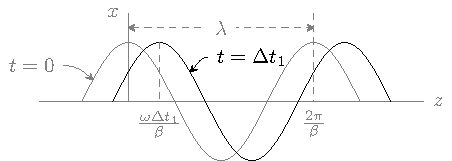
\includegraphics{figWaveMovingRightWithTime}
\caption{وقت $t=0$ اور $t=t_1$ پر خلاء میں موج کا مقام۔}
\label{شکل_موج_وقت_کے_ساتھ_مثبت_چلتی_موج}
\end{figure}


موج کی مساوات  میں \عددیء{\alpha=0} تصور کرتے ہوئے اسے وقت \عددیء{t=0} پر شکل \حوالہ{شکل_موج_وقت_کے_ساتھ_مثبت_چلتی_موج} میں ہلکی سیاہی سے دکھایا گیا ہے۔یہاں دھیان رہے کہ شکل میں \عددیء{z} محدد کو افقی دکھایا گیا ہے۔جیسے آپ دیکھ سکتے ہیں \عددیء{t=0} پر موج کی دو آپس میں قریبی چوٹیاں \عددیء{z=0} اور \عددیء{z=\tfrac{2\pi}{\beta}} پر پائی جاتی ہیں۔دو آپس میں قریبی چوٹیوں کے درمیان فاصلے کو \اصطلاح{طول موج}\فرہنگ{طول موج}\فرہنگ{موج!طول}\حاشیہب{wavelength}\فرہنگ{wavelength} پکارا اور \عددیء{\lambda} سے ظاہر کیا جاتا ہے۔یوں اس موج کی طول موج
\begin{align}\label{مساوات_موج_زاویائی_مستقل_اور_طول_موج_الف}
\lambda=\frac{2\pi}{\beta}
\end{align}
ہے جس سے
\begin{align}\label{مساوات_موج_زاویائی_مستقل_اور_طول_موج_ب}
\beta=\frac{2\pi}{\lambda}
\end{align}
لکھا جا سکتا ہے جو انتہائی اہم نتیجہ ہے۔

موج کی مساوات ہی کو وقت \عددیء{t=\Delta t_1} پر شکل \حوالہ{شکل_موج_وقت_کے_ساتھ_مثبت_چلتی_موج} میں دوبارہ گاڑھی سیاہی میں بھی دکھایا گیا ہے۔آپ دیکھ سکتے ہیں کہ اس دورانیے میں موج نے دائیں جانب یعنی \عددیء{z} بڑھنے کی طرف حرکت کی ہے۔یوں صاف ظاہر ہے کہ یہ موج وقت کے ساتھ مثبت \عددیء{z} جانب حرکت کر رہی ہے۔ دورانیہ \عددیء{\Delta t_1} میں موج کی چوٹی نے \عددیء{\tfrac{\omega \Delta t_1}{\beta}} فاصلہ طے کیا ہے لہٰذا موج کے رفتار کو
\begin{align}\label{مساوات_موج_رفتار_اور_تعدد}
v=\frac{\Delta z}{\Delta t}=\frac{\omega \Delta t_1}{\beta} \frac{1}{\Delta t_1}=\frac{\omega}{\beta}
\end{align}
لکھا جا سکتا ہے۔

مساوات \حوالہ{مساوات_موج_زاویائی_مستقل_اور_طول_موج_ب} کو  مساوات \حوالہ{مساوات_موج_رفتار_اور_تعدد} میں پر کرنے سے
\begin{align}
v=f \lambda
\end{align}
حاصل ہوتا ہے جو \عددیء{\lambda} طول موج  اور \عددیء{f} تعدد رکھنے والے موج کی رفتار \عددیء{v} دیتی ہے۔

مساوات \حوالہ{مساوات_موج_کوسائن_مثبت_موج} میں مساوات \حوالہ{مساوات_موج_رفتار_اور_تعدد} استعمال کرتے ہوئے
\begin{align}
E_x=E_0 e^{-\alpha z} \cos \left[ \omega \left(t-\frac{z}{v} \right)\right]
\end{align}
حاصل ہوتا ہے جسے مساوات \حوالہ{مساوات_موج_رفتار_اور_تعدد} اور مساوات \حوالہ{مساوات_موج_زاویائی_مستقل_اور_طول_موج_ب} کی مدد سے
\begin{align}
E_x=E_0 e^{-\alpha z} \cos \left(\omega  t-\frac{2 \pi z}{\lambda}\right)
\end{align}
بھی لکھا جا سکتا ہے۔

موج کی رفتار کو مساوات \حوالہ{مساوات_موج_کوسائن_مثبت_موج} سے دوبارہ حاصل کرتے ہیں۔اس مساوات کے تحت کسی بھی لمحہ \عددیء{t} پر موج کی چوٹی اس مقام پر ہو گی جہاں
\begin{align*}
\omega t -\beta z=0
\end{align*}
ہو۔چونکہ رفتار \عددیء{\tfrac{\dif z}{\dif t}} کو کہتے ہیں لہٰذا اس مساوات کے تفرق
\begin{align*}
\omega \dif t-\beta \dif z=0
\end{align*}
سے رفتار
\begin{align}
v=\frac{\dif z}{\dif t}=\frac{\omega}{\beta}
\end{align}
حاصل ہوتی ہے۔

\begin{figure}
\centering
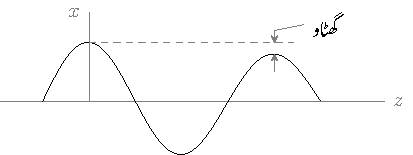
\includegraphics{figWaveAttenuation}
\caption{موج چلتے ہوئے آہستہ آہستہ کمزور ہوتی رہتی ہے۔}
\label{شکل_موج_کمزوری}
\end{figure}

شکل \حوالہ{شکل_موج_کمزوری} میں \عددیء{\alpha} کو صفر تصور نہیں کیا گیا ہے۔جیسا کہ آپ دیکھ سکتے ہیں، ایسی صورت میں موج کی چوٹی، \عددیء{z} کے ساتھ بتدریج گھٹتی  ہے لہٰذا \عددیء{{\alpha=\SI{0.001}{\neper \per \meter}}} کی صورت میں \عددیء{\SI{1}{\kilo \meter}} کے فاصلے پر موج کی چوٹی، ابتدائی چوٹی کے \عددیء{\tfrac{e^{-1}}{e^{-0}}=0.368} گنا رہ گئی ہو گی جہاں ابتدائی چوٹی \عددیء{z=0} پر لی گئی ہے۔

برقی موج \عددیء{\kvec{E}_{s}} سے مساوات \حوالہ{مساوات_موج_میکس_ویل_دوری_سمتیہ_شکل_الف}
\begin{align*}
\nabla \times \kvec{E}_{s}=-j \omega \mu \kvec{H}_{s}
\end{align*}
 کی مدد سے مقناطیسی موج با آسانی حاصل ہوتی ہے۔مساوات \حوالہ{مساوات_موج_مثبت_زیڈ_جانب_سمتی} استعمال کرتے ہوئے مندرجہ بالا مساوات سے
\begin{align*}
-\gamma E_0 e^{-\gamma z} \ay=-j \omega \mu \kvec{H}_s
\end{align*}
یا
\begin{align*}
\kvec{H}_s=\frac{\gamma}{j \omega \mu} E_0 e^{-\gamma z} \ay
\end{align*}
حاصل ہوتا ہے جس میں مساوات \حوالہ{مساوات_موج_حرکی_مستقل_الف} سے مثبت \عددیء{\gamma} کی قیمت پر کرنے سے
\begin{gather}
\begin{aligned}\label{مساوات_موج_مقناطیسی_جزو}
\kvec{H}_s&=\sqrt{\frac{\sigma +j \omega \epsilon}{j \omega \mu}} E_0 e^{-\gamma z} \ay\\
&=\frac{E_0}{\eta} e^{-\gamma z}\ay
\end{aligned}
\end{gather}
ملتا ہے جہاں دوسرے قدم پر
\begin{align}\label{مساوات-موج_قدرتی_رکاوٹ}
\eta =\sqrt{\frac{j \omega \mu}{\sigma +j \omega \epsilon}}
\end{align}
لکھی\حاشیہد{یونانی حروف تہجی \عددیء{\eta} ایٹا پڑھا جاتا ہے۔} گئی\حاشیہب{\عددیء{\eta}، eta} ہے۔اس مساوات کو
\begin{align}\label{مساوات-موج_قدرتی_رکاوٹ_ب}
\eta =\sqrt{\frac{\mu}{\epsilon}}\frac{1}{\sqrt{1-j \frac{\sigma}{\omega \epsilon}}}
\end{align}
بھی لکھا جا سکتا ہے۔

مساوات \حوالہ{مساوات_موج_مثبت_زیڈ_جانب_سمتی} کی غیر سمتی صورت یعنی \عددیء{E_{xs}=E_0e^{-\gamma z}} کو مساوات \حوالہ{مساوات_موج_مقناطیسی_جزو} کے غیر سمتی صورت یعنی \عددیء{H_{ys}=\tfrac{E_0}{\eta}e^{-\gamma z}} سے تقسیم کرتے ہوئے
\begin{align}
\frac{E_{xs}}{H_{ys}}=\eta
\end{align}
ملتا ہے۔

یہاں ذرہ رک کر ایک برقی دور پر غور کرتے ہیں۔منبع برقی دباو \عددیء{V_0 \cos (\omega t -\psi)} جسے دوری سمتیہ \عددیء{V_0 e^{-j\psi}} لکھا جا سکتا ہے کے ساتھ سلسلہ وار مزاحمت \عددیء{R}، امالہ \عددیء{L} اور کپیسٹر \عددیء{C} جڑے ہیں جن کی رکاوٹ \عددیء{Z}
\begin{align*}
Z=R+j\left( \omega L -\frac{1}{\omega C}\right)=R+jX=\abs{Z} e^{j \theta_Z}=\abs{Z}\phase{\theta_Z}
\end{align*}
لکھی جا سکتی ہے  جہاں \عددیء{\omega L > \tfrac{1}{\omega C}} کی صورت میں \عددیء{X} مثبت ہو گا جبکہ \عددیء{\omega L < \tfrac{1}{\omega C}} کی صورت میں یہ منفی ہو گا۔مزید \عددیء{\omega L = \tfrac{1}{\omega C}} کی صورت میں دور خالص مزاحمتی رکاوٹ پیش کرے گا اور \عددیء{\theta_Z=0} ہو گا۔اس دور میں برقی رو دوری سمتیہ کی مدد سے
\begin{align*}
I_s=\frac{V_s}{Z_s}=\frac{V_0 e^{-j\psi}}{\abs{Z}e^{j \theta_Z}}=\frac{V_0}{\abs{Z}}e^{-j(\psi+\theta_Z)}
\end{align*}
حاصل ہوتا ہے جس سے
\begin{align*}
i=\frac{V_0}{\abs{Z}}\cos \left(\omega t -\psi-\theta_Z \right)
\end{align*}
لکھا جا سکتا ہے۔برقی دباو اور برقی رو ایک ہی تعدد رکھتے ہیں البتہ ان میں زاویائی فاصلہ \عددیء{\theta_Z} پایا جاتا ہے۔مثبت \عددیء{X} کی صورت میں برقی رو اس زاویائی فاصلے کے برابر برقی دباو کے پیچھے رہتی ہے جبکہ منفی \عددیء{X} کی صورت میں برقی رو اس زاویائی فاصلے کے برابر برقی دباو کے آگے رہتی ہے۔ہم دیکھتے ہیں کہ برقی دباو اور برقی رو کی شرح
\begin{align*}
\frac{V_s}{I_s}=\abs{Z} e^{j \theta_Z}=Z
\end{align*}
کے برابر ہے جسے رکاوٹ کہتے ہیں۔

آئیں اب دوبارہ امواج کی بات کریں۔برقی موج کو اس مثال کے برقی دباو کی جگہ اور مقناطیسی موج کو مثال کے رو کی جگہ رکھتے ہوئے آپ دیکھیں گے کہ دونوں مسائل ہوبہو یکساں ہیں۔اسی وجہ سے  برقی موج \عددیء{E_{xs}} اور مقناطیسی موج \عددیء{H_{ys}} کی شرح \عددیء{\eta}،  \اصطلاح{قدرتی رکاوٹ}\فرہنگ{قدرتی رکاوٹ}\فرہنگ{رکاوٹ!قدرتی}\حاشیہب{intrinsic impedance}\فرہنگ{intrinsic impedance} کہلاتی ہے۔بالکل برقی رکاوٹ کی طرح قدرتی رکاوٹ حقیقی یا خیالی اور یا مخلوط عدد ہو سکتا ہے۔قدرتی رکاوٹ کی اکائی اوہم \عددیء{\si{\ohm}} ہے۔

مساوات \حوالہ{مساوات_موج_مقناطیسی_جزو} سے مقناطیسی موج
\begin{align}\label{مساوات_موج_عمومی_مقناطیسی}
H_y=\frac{E_0 e^{-\alpha z}}{\abs{\eta}} \cos \left(\omega t - \beta z -\theta_{\eta} \right)
\end{align}
لکھی جائے گی جہاں قدرتی رکاوٹ کو
\begin{align}
\eta=\abs{\eta} e^{j \theta_{\eta}}
\end{align}
لکھا گیا۔

مساوات \حوالہ{مساوات_موج_کوسائن_مثبت_موج} کے تحت برقی میدان \عددیء{x} محدد کے متوازی ہے جبکہ مساوات \حوالہ{مساوات_موج_عمومی_مقناطیسی} کے تحت مقناطیسی میدان \عددیء{y} محدد کے متوازی ہے لہٰذا یہ میدان  آپس میں ہر وقت عمودی رہتے ہیں۔اس کے علاوہ دونوں امواج \عددیء{z} سمت میں حرکت کر رہے ہیں۔یوں میدان کی سمت اور حرکت کی سمت بھی آپس میں عمودی ہیں۔ایسے امواج جن میں میدان کی سمت اور حرکت کی سمت عمودی ہوں \اصطلاح{عرضی امواج}\فرہنگ{عرضی!موج}\فرہنگ{موج!عرضی}\حاشیہب{transverse waves}\فرہنگ{transverse waves} کہلاتے ہیں۔پانی کی سطح پر لہریں بھی عرضی امواج ہوتے ہیں۔اسی طرح رسی کو کھینچ کر رکھتے ہوئے اسے جھٹکے  سے ہلانے سے  رسی میں عرضی موج پیدا ہوتی ہے۔\اصطلاح{عرضی برقی و مقناطیسی موج}\فرہنگ{عرضی!برقی و مقناطیسی}\حاشیہب{transverse electromagnetic, TEM}\فرہنگ{transverse electromagnetic}\فرہنگ{TEM} میں برقی میدان اور مقناطیسی میدان دونوں حرکت کے سمت کے عمودی ہوتے ہیں۔ باب \حوالہ{باب_مویج} میں ایسے امواج پر غور کیا جائے گا جن میں صرف ایک میدان سمت حرکت کے عمودی ہو گا۔انہیں \اصطلاح{عرضی برقی موج}\حاشیہب{transverse electric wave, TE wave} یا \اصطلاح{عرضی مقناطیسی موج}\حاشیہب{transverse magnetic wave, TM wave} کا نام دیا گیا ہے۔ 

آئیں اب چند مخصوص صورتوں میں ان مساوات کو استعمال کرنا سیکھیں۔
%====================
\جزوحصہ{خالی خلاء میں امواج}
خالی خلاء میں \عددیء{\sigma=0}، \عددیء{\mu_R=1} اور \عددیء{\epsilon_R=1}  ہیں لہٰذا مساوات \حوالہ{مساوات_موج_حرکی_مستقل_الف} سے مثبت حرکی مستقل
\begin{align*}
\gamma=\sqrt{j \omega \mu_R \mu_0  \left(\sigma +j \omega \epsilon_R \epsilon_0 \right)}=j \omega \sqrt{\mu_0 \epsilon_0}
\end{align*}
حاصل ہوتا ہے جس سے
\begin{align*}
\alpha&=0\\
\beta&=\omega \sqrt{\mu_0 \epsilon_0}
\end{align*}
حاصل ہوتے ہیں۔چونکہ خالی خلاء میں  \عددی{\alpha=0} ہے لہٰذا خالی خلاء بے ضیاع خطہ ہے۔یوں خالی خلاء میں برقی و مقناطیسی امواج کی رفتار، جسے روایتی طور پر \عددیء{c} سے ظاہر کیا جاتا ہے،  مساوات \حوالہ{مساوات_موج_رفتار_اور_تعدد} سے
\begin{align}
c=\frac{\omega}{\beta}=\frac{1}{\sqrt{\mu_0 \epsilon_0}}
\end{align}
حاصل ہوتی ہے جس کی قیمت
\begin{align*}
c=\frac{1}{\sqrt{4 \times \pi \times 10^{-7} \times 8.854 \times 10^{-12}}}&=\SI{2.99e8}{\meter \per \second} \\
&\approx \SI{3e8}{\meter \per \second}
\end{align*}
ہے۔

مساوات \حوالہ{مساوات-موج_قدرتی_رکاوٹ} سے خالی خلاء کی قدرتی رکاوٹ
\begin{align*}
\eta =\sqrt{\frac{j \omega \mu_R \mu_0}{\sigma +j \omega \epsilon_R \epsilon_0}}=\sqrt{\frac{\mu_0}{\epsilon_0}}
\end{align*}
حاصل ہوتی ہے۔قدرتی رکاوٹ کی قیمت حاصل کرنے کی خاطر ہم \عددیء{\tfrac{1}{4\pi \epsilon_0}=9\times 10^9} سے \عددیء{\epsilon_0=\tfrac{1}{36\pi 10^9}} لکھتے ہوئے
\begin{align}
\eta=120 \pi \approx \SI{377}{\ohm}
\end{align}
حاصل کرتے ہیں۔یوں خالی خلاء میں کسی بھی لمحے، کسی بھی نقطے پر برقی میدان کی قیمت اس نقطے پر مقناطیسی میدان کے \عددیء{377} گنا ہو گی۔

حرکی مستقل اور قدرتی رکاوٹ کی قیمتیں استعمال کرتے ہوئے خالی خلاء میں متحرک موج کے میدان
\begin{align*}
E_x&=E_0 \cos \left[\omega \left( t -\frac{z}{c} \right)\right]\\
H_y&=\frac{E_0}{120 \pi} \cos \left[ \omega \left( t -\frac{z}{c} \right) \right]
\end{align*}
لکھے جائیں گے۔آپ دیکھ سکتے ہیں کہ دونوں میدان ہم زاویہ ہیں۔یوں کسی بھی نقطے پر بڑھتے برقی میدان کی صورت میں اس نقطے پر مقناطیسی میدان بھی بڑھتا ہے۔ان مساوات کے تحت امواج بالکل سیدھے حرکت کرتے ہیں اور نا وقت اور نا ہی فاصلے کے ساتھ ان کی طاقت میں کسی قسم کی کمی رونما ہوتی ہے۔یہی وجہ ہے کہ کائنات کے دور ترین کہکشاوں سے ہم تک برقی و مقناطیسی امواج پہنچتی ہیں اور ہمیں رات کے چمکتے اور خوبصورت تارے نظر آتے ہیں۔

%=========================

\ابتدا{مشق}
\اصطلاح{بے تار}\فرہنگ{بے تار}\حاشیہب{wireless}\فرہنگ{wireless} ذرائع ابلاغ میں \عددیء{\SI{36000}{\kilo \meter}} کی اونچائی پر پرواز کرتے مصنوعی سیارے اہم کردار ادا کرتے ہیں۔یہ سیارے زمین کے اوپر ایک ہی نقطے پر آویزاں نظر آتے ہیں۔ان سیاروں سے زمین کے قریبی نقطے تک برقی اشارہ کتنی دیر میں پہنچے گا۔

جواب:\عددیء{\SI{0.12}{\second}}
\انتہا{مشق}
%=========================
\ابتدا{مثال}
خالی خلاء میں \عددی{\SI{240}{\mega\hertz}} تعدد کی موج بڑھتے \عددی{\az} سمت میں حرکت کر رہی ہے۔الف) \عددی{\lambda}، \عددی{\beta} اور \عددی{\omega} دریافت کریں۔ ب) لمحہ \عددی{{t=0}} پہ موج کی \عددی{\SI{128}{\volt\per\meter}} چوٹی  محدد کے مرکز پر پائی جاتی ہے۔موج کی حقیقی اور دوری مساوات لکھیں۔ پ) اگر موج کی چوٹی لمحہ \عددی{t=\SI{1.2}{\nano\second}} پر نقطہ \عددی{z=\SI{25}{\centi\meter}} پہ ہو تب موج کی مساوات کیا ہو گی؟ 

حل:الف) موج کی رفتار \عددی{c=\SI{3e8}{\meter\per\second}} لیتے ہوئے 
\begin{align*}
\lambda=\frac{c}{f}=\frac{3\times 10^8}{240\times 10^6}=\frac{5}{4}\si{\meter}
\end{align*}
اور یوں
\begin{align*}
\beta=\frac{2\pi}{\lambda}=\frac{8\pi}{5}\si{\radian \per\meter}
\end{align*}
حاصل ہوتے ہیں۔اب زاویائی تعدد حاصل کرتے ہیں۔
\begin{align*}
\omega= 2\pi f =4.8\pi \times 10^{8} \si{\radian \per \second}
\end{align*}
ب) حقیقی مساوات 
\begin{align*}
E=128 \cos \left(4.8\pi \times 10^8 t -\frac{8\pi }{5} z \right)
\end{align*}
ہے جبکہ دوری مساوات مندرجہ ذیل ہے۔
\begin{align*}
E=128 e^{-j\frac{8\pi }{5} z}
\end{align*}
پ) اب موج تاخیر سے محدد کے مرکز پر پہنچتی ہے۔موج کا تاخیری زاویہ \عددی{\theta} لکھتے ہوئے موج کی مساوات
\begin{align*}
E=128 \cos \left(4.8\pi \times 10^8 t -\frac{8\pi }{5} z +\theta \right)
\end{align*}
ہو گی۔موج کی چوٹی \عددی{(4.8\pi \times 10^8 t -\frac{8\pi }{5} z +\theta)=0} پر ہو گی لہٰذا \عددی{t=\SI{1.2}{\nano\second}} اور \عددی{z=\SI{0.25}{\meter}} پر کرتے ہوئے  \عددی{\theta=-0.176\pi} حاصل ہوتا ہے۔یہ قیمت مندرجہ بالا مساوات میں استعمال کی جائے گی۔موج کی دوری مساوات مندرجہ ذیل ہے۔
\begin{align*}
E_s=128 e^{-j \pi (\frac{8}{5} z +0.176) }
\end{align*} 
\انتہا{مثال}
%===========================
\ابتدا{مثال}\شناخت{مثال_مستوی_موج_برقی_میدان_مساوات}
لمحہ \عددی{t=0} پہ محدد کے مرکز پر موج کی چوٹی \عددی{\SI{340}{\volt\per\meter}} پائی جاتی ہے جبکہ \عددی{z=\SI{1.5}{\meter}} وہ قریب ترین نقطہ ہے جہاں میدان صفر کے برابر ہے۔موج گھٹے \عددی{z} کی سمت میں حرکت کر رہی ہے۔اس لمحہ برقی میدان اکائی
 سمتیہ \عددی{\kvec{a}_E=\tfrac{2}{\sqrt{13}}\ax+\tfrac{3}{\sqrt{13}}\ay} کی سمت میں ہے۔ برقی موج کی مساوات لکھیں۔

حل:موج کی چوٹی اور صفر کے درمیان فاصلے سے \عددی{\tfrac{\lambda}{4}=1.5} لکھ کر \عددی{{\lambda=\SI{6}{\meter}}} حاصل ہوتا ہے جس کو استعمال کرتے ہوئے ہم  \عددی{{\beta=\tfrac{2\pi}{\lambda}=\tfrac{\pi}{3}}}  اور \عددی{f=\tfrac{3\times 10^8}{6}=\SI{50}{\mega\hertz}} حاصل کرتے  ہیں۔ چونکہ موج گھٹتے \عددی{z} جانب حرکت کر رہی ہے اور لمحہ \عددی{t=0} پر اس کی چوٹی محدد کے مرکز پر پائی جاتی ہے  لہٰذا 
\begin{align*}
\kvec{E}=\kvec{E}_0 \cos \left(2\pi \times 50 \times 10^6 t + \frac{\pi}{3} z \right)
\end{align*}
لکھا جائے گا۔لمحہ \عددی{t=0} پر محدد کے مرکز پر میدان \عددی{340 \kvec{a}_E} پایا جاتا ہے لہٰذا موج کی مکمل خاصیت مندرجہ ذیل مساوات بیان کرے گی۔ 
\begin{align*}
\kvec{E}=340\left[\tfrac{2}{\sqrt{13}}\ax+\tfrac{3}{\sqrt{13}}\ay\right] \cos \left(2\pi \times 50 \times 10^6 t + \frac{\pi}{3} z \right)
\end{align*}
اس کی دوری شکل مندرجہ ذیل ہے۔
\begin{align*}
\kvec{E}_s=340\left[\tfrac{2}{\sqrt{13}}\ax+\tfrac{3}{\sqrt{13}}\ay\right] e^{j\frac{\pi}{3} z}
\end{align*}
\انتہا{مثال}
%=======================
\ابتدا{مثال}
خالی خلاء میں برقی موج \عددی{\kvec{E}_s=340\left[\tfrac{2}{\sqrt{13}}\ax+\tfrac{3}{\sqrt{13}}\ay\right] e^{j\frac{\pi}{3} z}} پائی جاتی ہے۔مقناطیسی موج کی مساوات لکھیں۔

حل:خالی خلاء میں
\begin{align*}
\frac{E_0}{H_0}=\sqrt{\frac{\mu_0}{\epsilon_0}} =120\pi
\end{align*} 
سے مقناطیسی چوٹی کی قیمت 
\begin{align*}
H_0=\frac{340}{120\pi}=\frac{17}{6\pi}
\end{align*}
حاصل ہوتی ہے۔یہ حقیقی عدد ہے لہٰذا برقی اور مقناطیسی میدان ہم قدم ہیں۔خالی خلاء میں موج کے برقی اور مقناطیسی میدان آپس میں عمودی ہوتے ہیں۔یوں مقناطیسی موج کی سمت میں سمتیہ \عددی{x\ax+y\ay} اور  برقی موج کی سمت میں سمتیہ \عددی{\kvec{a}_E} کا غیر سمتی ضرب صفر کے برابر ہو گا یعنی
\begin{align*}
\left(\frac{2}{\sqrt{13}}\ax+\frac{3}{\sqrt{13}}\ay\right) \cdot (x \ax+y \ay)=0
\end{align*}
ہو گا جس سے
\begin{align}\label{مساوات_مستوی_موج_برقی_مقناطیسی_عمودی_اکائی}
2x+3y=0
\end{align}
حاصل ہوتا ہے۔اس میں \عددی{x} کی کوئی بھی قیمت پر کرتے ہوئے \عددی{y} کی قیمت حاصل ہوتی ہے۔یوں \عددی{x=1} پر کرنے سے \عددی{y=-\tfrac{2}{3}} حاصل ہوتا ہے۔یوں مقناطیسی میدان  \عددی{1\ax-\tfrac{2}{3}\ay} سمتیہ کی سمت میں ہو گی۔ اس طرح مقناطیسی میدان کی سمت میں اکائی سمتیہ
\begin{align*}
\kvec{a}_H=\frac{\ax-\frac{2}{3}\ay}{\sqrt{1+\frac{4}{9}}}=\frac{3}{\sqrt{13}}\ax-\frac{2}{\sqrt{13}}\ay
\end{align*}
ہو گی۔یاد رہے کہ \عددی{\kvec{a}_E \times \kvec{a}_H} سے موج کے حرکت کی سمت حاصل ہوتی ہے۔ہم دیکھتے ہیں کہ
\begin{align*}
\kvec{a}_E \times \kvec{a}_H=(\frac{2}{\sqrt{13}}\ax+\frac{3}{\sqrt{13}}\ay) \times (\frac{3}{\sqrt{13}}\ax-\frac{2}{\sqrt{13}}\ay)=-\az
\end{align*}
کے برابر ہے جو موج کی درست سمت ہے۔اب ہم مساوات \حوالہ{مساوات_مستوی_موج_برقی_مقناطیسی_عمودی_اکائی} میں \عددی{x} کی قیمت منفی بھی پر کر سکتے تھے۔آئیں ایسا بھی کر کے دیکھ لیں۔اگر ہم \عددی{x=-1} پر کرتے تب \عددی{y=\tfrac{2}{3}} حاصل ہوتا جس سے اکائی سمتیہ \عددی{-1\ax+\tfrac{2}{3}\ay}  حاصل ہوتی۔اس اکائی سمتیہ اور \عددی{\kvec{a}_E} کے سمتی ضرب سے \عددی{\az} حاصل ہوتا ہے جو بالکل الٹ سمت میں حرکت کرتی موج کی سمت ہے۔ظاہر ہے کہ ہم ان دو جوابات میں سے پہلی جواب کو ہی یہاں درست تسلیم کریں گے۔یوں مقناطیسی موج کی دوری مساوات مندرجہ ذیل ہو گی۔
\begin{align*}
\kvec{H}_s=H_0 \kvec{a}_H e^{j\frac{\pi}{3} z}=\frac{17}{6\pi} \left(\frac{3}{\sqrt{13}}\ax-\frac{2}{\sqrt{13}}\ay \right)e^{j\frac{\pi}{3} z}
\end{align*}
 
\انتہا{مثال}
%===========================
\جزوحصہ{خالص یا کامل ذو برق میں امواج}
خالص یا کامل ذو برقی سے مراد ایسا ذو برق ہے جس میں متحرک برقی و مقناطیسی امواج کی توانائی ضائع نہیں ہوتی۔خالص ذو برق میں \عددیء{\sigma=0} جبکہ اس کا جزوی مقناطیسی مستقل \عددیء{\mu_R} اور جزوی برقی مستقل \عددیء{\epsilon_R}  ہے لہٰذا مساوات \حوالہ{مساوات_موج_حرکی_مستقل_الف} سے مثبت حرکی مستقل
\begin{align*}
\gamma=j \omega \sqrt{\mu \epsilon }
\end{align*}
حاصل ہوتا ہے جس سے
\begin{align}
\alpha&=0\\
\beta&=\omega \sqrt{\mu \epsilon} \label{مساوات_موج_کامل-ذوبرق_بیٹا}
\end{align}
حاصل ہوتے ہیں۔کامل ذو برق میں \عددی{\alpha=0} ہے لہٰذا کامل ذو برق بے ضیاع ہے۔ یوں خالی خلاء میں برقی و مقناطیسی امواج کی رفتار  مساوات \حوالہ{مساوات_موج_رفتار_اور_تعدد} سے
\begin{align}
v=\frac{\omega}{\beta}=\frac{1}{\sqrt{\mu_R \mu_0 \epsilon_R \epsilon_0}}=\frac{c}{\sqrt{\mu_R \epsilon_R}}
\end{align} 
حاصل ہوتی ہے جہاں \عددیء{\tfrac{1}{\sqrt{\mu_0 \epsilon_0}}} کو خالی خلاء میں روشنی کی رفتار \عددیء{c} لکھا گیا ہے۔چونکہ ذو برق میں \عددیء{\mu_R \epsilon_R > 1} ہے  لہٰذا ذو برق میں روشنی کی رفتار خالی خلاء میں روشنی کے رفتار سے کم ہو گی۔خالی خلاء میں روشنی کی رفتار اس کی زیادہ سے زیادہ رفتار ہے۔

موج کی رفتار اور تعدد سے طول موج
\begin{align}
\lambda=\frac{v}{f}=\frac{c}{f \sqrt{\mu_R \epsilon_R}}=\frac{\lambda_0}{\sqrt{\mu_R \epsilon_R}}
\end{align}
حاصل ہوتی ہے جہاں خالی خلاء کے طول موج کو \عددیء{\lambda_0} لکھا گیا ہے۔اس مساوات سے ذو برق میں روشنی کی رفتار کم ہونے کی وجہ سامنے آتی ہے۔چونکہ \عددیء{\mu_R \epsilon_R >1} ہے لہٰذا ذو برق میں طول موج کم ہو جاتا ہے جس سے روشنی کی رفتار کم ہو جاتی ہے۔


مساوات \حوالہ{مساوات-موج_قدرتی_رکاوٹ} سے ذو برقی کی  قدرتی رکاوٹ
\begin{align*}
\eta =\sqrt{\frac{\mu}{\epsilon}}=\sqrt{\frac{\mu_0}{\epsilon_0}}\sqrt{\frac{\mu_R}{\epsilon_R}}= \eta_0 \sqrt{\frac{\mu_R}{\epsilon_R}}
\end{align*}
حاصل ہوتی ہے جہاں خالی خلاء کی قدرتی رکاوٹ کو \عددیء{\eta_0} لکھا گیا ہے۔

یوں ذو برق میں امواج کے مساوات
\begin{align}
E_x&=E_0 \cos (\omega t -\beta z)\\
H_y&=\frac{E_0}{\eta} \cos (\omega t -\beta z)
\end{align}
ہیں۔

%==================
\ابتدا{مثال}
پانی کے لئے \عددیء{\mu_R=1}، \عددیء{\epsilon_R=78.4} اور \عددیء{\sigma=0} لیتے ہوئے \عددیء{\SI{300}{\mega \hertz}} تعدد کے برقی و مقناطیسی امواج کی رفتار، طول موج اور قدرتی رکاوٹ حاصل کریں۔ برقی میدان \عددیء{\SI{50}{\milli \volt \per \meter}} ہونے کی صورت میں برقی اور مقناطیسی امواج کے مساوات لکھیں۔ہم \عددیء{\sigma=0} لیتے ہوئے درحقیقت پانی میں توانائی کے ضیاع کو نظرانداز کر رہے ہیں۔

حل:
\begin{align*}
v=\frac{c}{\sqrt{\mu_R \epsilon_R}}=\frac{3 \times 10^8}{\sqrt{78.4}}=\SI{0.3388e8}{\meter \per \second}\\
\lambda=\frac{v}{f}=\frac{0.3388 \times 10^8}{300 \times 10^6}=\SI{11.29}{\centi\meter}
\end{align*}
ہیں جبکہ خالی خلاء میں \عددیء{\lambda=\SI{1}{\meter}} ہے۔بقایا مستقل
\begin{align*}
\beta=\frac{2\pi}{\lambda}=\SI{55.7}{\radian \per \meter}
\end{align*}
اور
\begin{align*}
\eta=\eta_0 \sqrt{\frac{\mu_R}{\epsilon_R}}=\frac{377}{\sqrt{78.4}}=\SI{42.58}{\ohm}
\end{align*}
ہیں۔امواج کے مساوات
\begin{align*}
E_x&=0.05 \cos (6\pi 10^8 t -55.7 z)\\
H_y&=\frac{0.05}{42.58} \cos (6\pi 10^8 t -55.7 z)=0.00117 \cos (6\pi 10^8 t -55.7 z)
\end{align*}
ہیں۔
\انتہا{مثال}
%===================
\ابتدا{مشق}
کتاب کے آخر میں مختلف اشیاء کے مستقل دئے گئے ہیں۔انہیں استعمال کرتے ہوئے  ابرق میں، طاقت کے ضیاع کو نظرانداز کرتے ہوئے،  \عددیء{\SI{5.6}{\giga\hertz}} اور \عددیء{\SI{10}{\milli \ampere \per \meter}} حیطے  کی مقناطیسی میدان پر مندرجہ ذیل حاصل کریں۔
\begin{itemize}
\item
موج کی رفتار،
\item
طول موج،
\item
زاویائی مستقل،
\item
قدرتی رکاوٹ،
\item
برقی میدان کا حیطہ۔
\end{itemize} 

جوابات:\عددیء{\SI{1.29e8}{\meter \per \second}}، \عددیء{\SI{23}{\centi\meter}}، \عددیء{\SI{272.6}{\radian \per \meter}}، \عددیء{\SI{162.1}{\ohm}} اور \عددیء{\SI{1.62}{\volt \per \meter}}
\انتہا{مشق}
%===================

\جزوحصہ{ناقص یا غیر کامل ذو برقی میں امواج}
کامل ذو برق میں امواج پر غور کے بعد فطری طور ناقص ذو برق پر بات کرنا ضروری ہے لہٰذا صاف پانی کو مثال بناتے ہوئے   \عددیء{\SI{20}{\giga \hertz}} تعدد پر  ایسا ہی کرتے ہیں۔صفحہ \حوالہصفحہ{شکل_موج_صاف_پانی_تعدد_بالمقابل_برقی_مستقل} پر شکل \حوالہ{شکل_موج_صاف_پانی_تعدد_بالمقابل_برقی_مستقل} میں صاف پانی کے مستقل دئے گئے ہیں۔

اس تعدد پر صاف پانی کے مستقل \عددیء{\epsilon_R=41} اور \عددیء{\sigma=\SI{36.7}{\siemens \per \meter}} ہیں۔چونکہ پانی غیر مقناطیسی ہے لہٰذا اس کا \عددیء{\mu_R=1} ہو گا۔ یوں
\begin{align*}
\frac{\sigma}{\omega \epsilon}=0.8
\end{align*}
اور
\begin{align*}
\gamma&=j 2\times \pi \times 20\times 10^9 \times \frac{\sqrt{1\times 41}}{3\times 10^8} \sqrt{1-j 0.8}\\
&=3035 \phase{70.67^{\circ}}\\
&=1005+j2864 \quad \si{\meter^{-1}}
\end{align*}
حاصل ہوتے ہیں۔یوں پانی کا تضعیفی مستقل
\begin{align*}
\alpha=\SI{1005}{\neper \per \meter}
\end{align*}
ہے جس کا مطلب ہے کہ پانی میں ہر \عددیء{\tfrac{1}{1005}} میٹر یعنی \عددیء{\SI{1}{\milli \meter}} فاصلہ طے  کرنے پر برقی اور مقناطیسی امواج \عددیء{0.368} گنا گھٹ جائیں گے۔پانی میں \عددی{\alpha \ne 0} ہے لہٰذا پانی ضیاع کار ہے۔آپ دیکھ سکتے ہیں \اصطلاح{ریڈار}\فرہنگ{ریڈار}\حاشیہب{radar}\فرہنگ{radar} پانی میں کیوں کام نہیں کرتا۔اسی طرح بارش کی صورت میں بھی ریڈار کی کارکردگی بری طرح متاثر ہوتی ہے۔پانی میں دیکھنے کی خاطر موج آواز استعمال کی جاتی ہیں۔

تضعیفی مستقل کو عموماً \اصطلاح{ڈیسی بیل}\فرہنگ{ڈیسی بیل}\حاشیہب{decibel, dB}\فرہنگ{decibel, dB} فی میٹر میں ناپا جاتا ہے جہاں \عددی{\SI{1}{\neper}=\SI{8.69}{\deci\bel}} کے برابر ہے۔یوں مندرجہ بالا جواب کو
\begin{align*}
\alpha=1005\times 8.69=\SI{8733}{\deci\bel\per\meter}
\end{align*}
بھی لکھا جا سکتا ہے۔

زاویائی مستقل
\begin{align*}
\beta=\SI{2864}{\radian \per \meter}
\end{align*}
ہے جو \عددیء{\sigma=0} کی صورت میں \عددیء{\SI{2682}{\radian \per \meter}} حاصل ہوتا ہے لہٰذا پانی کے موصلیت سے زاویائی مستقل زیادہ متاثر نہیں ہوا۔ اس تعدد پر خالی خلاء میں طول موج \عددیء{\SI{1.5}{\centi\meter}} ہے جبکہ پانی میں \عددیء{\lambda=\tfrac{2\pi}{\beta}} سے طول موج \عددیء{\SI{2.19}{\milli \meter}} ہے۔

قدرتی رکاوٹ
\begin{align*}
\eta=\frac{377}{\sqrt{41}}\frac{1}{\sqrt{1-j 0.8}}=52\phase{19.33^\circ}=49.1+j17.2 \quad \si{\ohm}
\end{align*}
ہے لہٰذا \عددیء{E_x} ہر نقطے پر \عددیء{H_y} سے \عددیء{19.33^\circ} آگے ہے۔


\begin{figure}
\centering
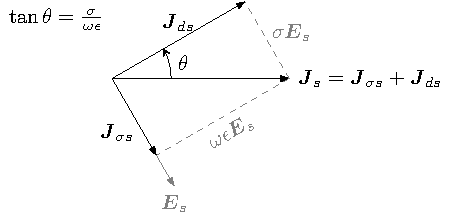
\includegraphics{figWaveLossTangent}
\caption{طاقت کے ضیاع کا تکون۔}
\label{شکل_موج_ضیاع_کا_تکون}
\end{figure}

میکس ویل کے مساوات
\begin{align*}
\nabla \times \kvec{H}_s=(\sigma+j\omega \epsilon)\kvec{E}_s=\kvec{J}_{\sigma s}+\kvec{J}_{d s}
\end{align*}
میں ایصالی اور انتقالی کثافت برقی رو کے سمتی مجموعے کو شکل \حوالہ{شکل_موج_ضیاع_کا_تکون} میں بطور مجموعی کثافت رو \عددیء{\kvec{J}_s} دکھایا گیا ہے۔ایصالی رو اور انتقالی رو آپس میں \عددیء{90^\circ} درجے کا زاویہ بناتے ہیں۔انتقالی رو \عددیء{90^\circ} آگے رہتا ہے۔یہ بالکل متوازی جڑے مزاحمت اور کپیسٹر کے رو کی طرح صورت حال ہے۔کپیسٹر کی رو، مزاحمت کی رو سے  \عددیء{90^\circ} آگے رہتی ہے۔مزید یہ کہ مزاحمت کی رو سے برقی طاقت  کا ضیاع پیدا ہوتا ہے جبکہ کپیسٹر کی رو سے ایسا نہیں ہوتا۔ان حقائق کو مد نظر رکھتے ہوئے  شکل \حوالہ{شکل_موج_ضیاع_کا_تکون} میں زاویہ \عددی{\theta} (جس کا کروی محدد کے زاویہ \عددیء{\theta} کے ساتھ کسی قسم کا کوئی تعلق نہیں ہے) کو دیکھیں جس کے لئے
\begin{align}
\tan \theta=\frac{\sigma}{\omega \epsilon}
\end{align}
لکھا جا سکتا ہے۔یوں اس تکون کو طاقت کے ضیاع کا تکون پکارا جاتا ہے اور \عددیء{\tfrac{\sigma}{\omega \epsilon}} کی شرح کو \اصطلاح{ضیاعی ٹینجنٹ}\فرہنگ{ضیاعی ٹینجنٹ}\حاشیہب{loss tangent}\فرہنگ{loss tangent} یا \اصطلاح{مماس ضیاع}\فرہنگ{مماس ضیاع}\فرہنگ{مماس!ضیاع}\فرہنگ{ضیاع!مماس}کہا جاتا ہے۔

مساوات \حوالہ{مساوات_موج_حرکی_مستقل_ب} اور مساوات \حوالہ{مساوات-موج_قدرتی_رکاوٹ_ب} کو \عددیء{\tfrac{\sigma}{\omega \epsilon}} استعمال کرتے ہوئے لکھا گیا۔کسی ذو برق کے کامل یا غیر کامل ہونے کا فیصلہ اس کے مماس ضیاع کی قیمت کو دیکھ کر کیا جاتا ہے۔اگر اس شرح کی قیمت اکائی کے قریب ہو تب ذو برق غیر کامل قرار دیا جاتا ہے جبکہ \عددیء{\tfrac{\sigma}{\omega \epsilon}\ll 1} کی صورت میں ذو برق کو کامل تصور کیا جاتا ہے۔

کم مماس ضیاع کی صورت میں حرکی مستقل اور قدرتی رکاوٹ کے کارآمد مساوات حاصل کئے جا سکتے ہیں۔حرکی مستقل
\begin{align*}
\gamma = j \omega \sqrt{\mu \epsilon}\sqrt{1-j \frac{\sigma}{\omega \epsilon}}
\end{align*}
کو \اصطلاح{مسئلہ ثنائی}\فرہنگ{مسئلہ ثنائی}\حاشیہب{binomial theorem}\فرہنگ{binomial theorem}
\begin{align*}
(1+x)^n=1+\frac{n}{1!}x+\frac{n(n-1)}{2!}x^2+\frac{n(n-1)(n-2)}{3!}x^3+\cdots
\end{align*}
جہاں \عددیء{\abs{x} <1} ہے، کی مدد سے  تسلسل کی شکل میں لکھ سکتے ہیں۔اگر ہم \عددیء{x=-\tfrac{\sigma}{\omega \epsilon}} اور \عددیء{n=\tfrac{1}{2}} لیں تو حرکی مستقل 
\begin{align*}
\gamma=j \omega \sqrt{\mu \epsilon} \left[1-j\frac{\sigma}{2\omega \epsilon}+\frac{1}{8}\left(\frac{\sigma}{\omega \epsilon}\right)^2+\cdots \right]
\end{align*}
 لکھا جا سکتا ہے جس سے
\begin{align}\label{مساوات_موج_تضعیفی_سادہ}
\alpha \overset{.}{=} j \omega \sqrt{\mu \epsilon} \left(-j\frac{\sigma}{2\omega \epsilon} \right)=\frac{\sigma}{2}\sqrt{\frac{\mu}{\epsilon}}
\end{align}
اور 
\begin{align}\label{مساوات_موج_زاویائی_سادہ_الف}
\beta \overset{.}{=}\omega \sqrt{\mu \epsilon}\left[1+\frac{1}{8}\left(\frac{\sigma}{\omega \epsilon}\right)^2 \right]
\end{align}
حاصل ہوتے ہیں۔اگر \عددیء{\tfrac{\sigma}{\omega \epsilon}\ll1} ہو تب
\begin{align}\label{مساوات_موج_زاویائی_سادہ_ب}
\beta \overset{.}{=}\omega \sqrt{\mu \epsilon}
\end{align}
بھی لکھا جا سکتا ہے۔بالکل اسی طرح قدرتی رکاوٹ کو
\begin{align}\label{مساوات_موج_رکاوٹ_سادہ_الف}
\eta \overset{.}{=} \sqrt{\frac{\mu}{\epsilon}} \left[1-\frac{3}{8}\left(\frac{\sigma}{\omega \epsilon}\right)^2 +j \frac{\sigma}{2\omega \epsilon}\right]
\end{align}
یا
\begin{align}\label{مساوات_موج_رکاوٹ_سادہ_ب}
\eta \overset{.}{=} \sqrt{\frac{\mu}{\epsilon}} \left(1 +j \frac{\sigma}{2\omega \epsilon}\right)
\end{align}
لکھا جا سکتا ہے۔

آئیں دیکھیں کہ ان مساوات سے حاصل جواب اصل مساوات کے جوابات کے کتنے قریب ہیں۔ایسا صاف پانی کی مثال کو دوبارہ حل کر کے دیکھتے ہیں۔ صاف پانی کے مستقل \عددیء{\عددیء{\SI{20}{\giga \hertz}}} تعدد پر \عددیء{\mu_R=1}، \عددیء{\epsilon_R=41} اور \عددیء{\sigma=\SI{36.7}{\siemens \per \meter}} ہیں لہٰذا  مساوات \حوالہ{مساوات_موج_تضعیفی_سادہ} سے
\begin{align*}
\alpha =\SI{1080}{\neper \per \meter} \quad \quad (\SI{9385}{\deci\bel\per\meter})
\end{align*}
حاصل ہوتا ہے جو گزشتہ حاصل کردہ قیمت \عددیء{\SI{1005}{\neper \per \meter}} کے کافی قریب ہے۔مساوات \حوالہ{مساوات_موج_زاویائی_سادہ_الف} سے
\begin{align*}
\beta=\SI{2897}{\radian \per \meter}
\end{align*}
حاصل ہوتا ہے جو گزشتہ جواب \عددیء{\SI{2864}{\radian \per \meter}} کے بہت قریب ہے۔مساوات \حوالہ{مساوات_موج_زاویائی_سادہ_ب} سے حاصل جواب
\begin{align*}
\beta=\SI{2682}{\radian \per \meter}
\end{align*}
درست جواب سے نسبتاً زیادہ مختلف ہے۔قدرتی رکاوٹ مساوات \حوالہ{مساوات_موج_رکاوٹ_سادہ_الف} سے
\begin{align*}
\eta=44.75+j 23.55
\end{align*}
حاصل ہوتا ہے جو \عددیء{49.1+j17.2} کے بہت قریب ہے البتہ مساوات \حوالہ{مساوات_موج_رکاوٹ_سادہ_ب} سے حاصل جواب
\begin{align*}
\eta=58.88+j23.55
\end{align*}
قدر مختلف ہے۔صاف پانی کی اس مثال میں مماس ضیاع \عددیء{0.8} ہے جو اکائی سے بہت کم نہیں ہے، اسی لئے جوابات پہلے سے قدر مختلف حاصل ہوئے۔چونکہ موصلیت اور برقی مستقل کی بالکل درست قیمتیں عموماً ہمیں معلوم نہیں ہوتیں لہٰذا سادہ مساوات سے حاصل جوابات کے اس فرق کو زیادہ اہمیت نہیں دینی چاہئے۔ بہتر یہی ہوتا ہے کہ \عددیء{\tfrac{\sigma}{\omega \epsilon}<0.1} ہی کی صورت میں سادہ مساوات استعمال کئے جائیں۔

عموماً ذو برق کی موصلیت تعدد بڑھانے  سے غیر خطی طور پر بڑھتی ہے جبکہ \عددیء{\tfrac{\sigma}{\omega \epsilon}} کے قیمت میں تبدیلی نسبتاً  کم ہوتی ہے۔یہی وجہ مماس ضیاع کی اہمیت کا راز ہے۔یاد رہے کہ مختلف تعدد پر موصلیت، برقی مستقل اور مماس ضیاع نہایت تیزی سے تبدیل ہو سکتے ہیں۔ایسا عموماً نظر آنے والی روشنی سے قدر کم یا قدر زیادہ تعدد پر ہوتا ہے۔ 

\begin{figure}
\centering
\includegraphics{figWaveOctaveWaterDielectricLoss}
\caption{صاف پانی کا جزوی برقی مستقل بالمقابل زاویائی تعدد اور موصلیت بالمقابل زاویائی تعدد۔}
\label{شکل_موج_صاف_پانی_تعدد_بالمقابل_برقی_مستقل}
\end{figure}

شکل \حوالہ{شکل_موج_صاف_پانی_تعدد_بالمقابل_برقی_مستقل} میں صاف پانی کا جزوی برقی مستقل \عددیء{\epsilon_R} بالمقابل زاویائی تعدد \عددیء{\omega} ٹھوس لکیر سے دکھایا گیا ہے جبکہ موصلیت بالمقابل تعدد نقطہ دار لکیر سے دکھایا گیا ہے۔افقی محدد تعدد کا لاگ ہے۔آپ دیکھ سکتے ہیں کہ تقریباً \عددیء{\SI{10}{\giga\radian\per\second}} تعدد تک \عددیء{\epsilon_R=78.4} رہتا ہے جبکہ اس سے بلند تعدد پر اس کی قیمت گھٹ کر \عددیء{2.4} ہو جاتی ہے۔موصلیت کی چوٹی تقریباً \عددیء{\SI{36.7}{\siemens \per \meter}} پائی جاتی ہے۔دیگر ذو برق کے خط مختلف اشکال کے ہوں گے۔
%=========================

%=========================
\ابتدا{مشق}
ایک مادے  کے مستقل \عددیء{\SI{1}{\mega \hertz}} تعدد پر  \عددیء{\mu_R=1}، \عددیء{\epsilon_R=2.8} اور \عددیء{\sigma=\SI{10}{\micro \siemens\per\meter}} ہیں۔ اس مادے کے مماس ضیاع، تضعیفی مستقل اور زاویائی مستقل حاصل کریں۔تضعیفی مستقل کی قیمت \عددی{\si{\deci\bel\per\meter}} میں کیا ہے۔

جوابات:\عددیء{0.0642}، \عددیء{\SI{1.13e-3}{\neper\per\meter}} اور \عددیء{\SI{3.51e-4}{ \radian\per\meter}}، \عددی{\SI{9.8e-3}{\deci\bel\per\meter}}
\انتہا{مشق}
%=========================
\ابتدا{مشق}
ایک غیر مقناطیسی مادے کا مماس ضیاع \عددیء{0.07} جبکہ \عددیء{\mu_R=4.7} ہیں۔ان قیمتوں کو \عددیء{\SI{1}{\mega\hertz}} تا \عددیء{\SI{80}{\mega\hertz}} تعدد کے درمیان اٹل تصور کیا جا سکتا ہے۔اس کا تضعیفی مستقل اور  مادے میں طول موج  \عددیء{\SI{20}{\mega\hertz}} اور \عددیء{\SI{60}{\mega\hertz}} تعدد پر حاصل کریں۔

جوابات:\عددیء{\SI{0.031}{\neper\per\meter}} یا \عددی{\SI{0.269}{\deci\bel\per\meter}}، \عددیء{\SI{6.9}{\meter}}، \عددیء{\SI{0.095}{\neper\per\meter}} یا \عددی{\SI{0.826}{\deci\bel\per\meter}}،  \عددیء{\SI{2.3}{\meter}}
\انتہا{مشق}
%=======================

\حصہ{پوئنٹنگ سمتیہ}
امواج کی طاقت جاننے کے لئے  \اصطلاح{مسئلہ پوئنٹنگ}\فرہنگ{مسئلہ!پوئنٹنگ}\فرہنگ{پوئنٹنگ!مسئلہ}\حاشیہب{Poynting theorem}\فرہنگ{Poynting theorem}\فرہنگ{theorem!Poynting}  درکار ہو گا لہٰذا پہلے اسے\حاشیہد{جان ہینری پوئنٹنگ نے  1884 میں پہلی بار اس مسئلے کو پیش کیا۔} حاصل کرتے ہیں۔

میکس ویل کے مساوات 
\begin{align*}
\nabla \times \kvec{H}=\kvec{J}+\frac{\partial \kvec{D}}{\partial t}
\end{align*}
کا \عددیء{\kvec{E}} کے ساتھ غیر سمتی ضرب
\begin{align*}
\kvec{E} \cdot \nabla \times \kvec{H}=\kvec{E} \cdot \kvec{J}+\kvec{E} \cdot \frac{\partial \kvec{D}}{\partial t}
\end{align*}
لیتے ہوئے سمتی مماثل (جسے آپ با آسانی کارتیسی محدد میں ثابت کر سکتے ہیں)
\begin{align*}
\nabla \cdot \left(\kvec{E} \times \kvec{H} \right)=-\kvec{E} \cdot \nabla \times \kvec{H}+\kvec{H} \cdot \nabla \times \kvec{E}
\end{align*}
کے ذریعہ
\begin{align*}
\kvec{H} \cdot \nabla \times \kvec{E}-\nabla \left(\kvec{E} \times \kvec{H}\right)=\kvec{E} \cdot \kvec{J}+\kvec{E} \cdot \frac{\partial \kvec{D}}{\partial t}
\end{align*}
حاصل ہوتا ہے۔اس میں \عددیء{\nabla \times \kvec{E}=-\tfrac{\partial \kvec{B}}{\partial t}} پر کرنے سے
\begin{align*}
-\kvec{H} \cdot \frac{\partial \kvec{B}}{\partial t}-\nabla \left(\kvec{E} \times \kvec{H}\right)=\kvec{E} \cdot \kvec{J}+\kvec{E} \cdot \frac{\partial \kvec{D}}{\partial t}
\end{align*}
یا
\begin{align*}
-\nabla \left(\kvec{E} \times \kvec{H}\right)=\kvec{E} \cdot \kvec{J}+\epsilon \kvec{E} \cdot \frac{\partial \kvec{E}}{\partial t}+\mu \kvec{H} \cdot \frac{\partial \kvec{H}}{\partial t}
\end{align*}
حاصل ہوتا ہے۔اب
\begin{align*}
\epsilon \kvec{E} \cdot \frac{\partial \kvec{E}}{\partial t}=\frac{\epsilon}{2}\frac{\partial E^2}{\partial t}=\frac{\partial}{\partial t} \left(\frac{\epsilon E^2}{2} \right)
\end{align*}
اور
\begin{align*}
\mu \kvec{H} \cdot \frac{\partial \kvec{H}}{\partial t}=\frac{\mu}{2}\frac{\partial H^2}{\partial t}=\frac{\partial}{\partial t} \left(\frac{\mu H^2}{2} \right)
\end{align*}
لکھے جا سکتے ہیں لہٰذا
\begin{align*}
-\nabla \left(\kvec{E} \times \kvec{H}\right)=\kvec{E} \cdot \kvec{J}+\frac{\partial}{\partial t} \left(\frac{\epsilon E^2}{2} + \frac{\mu H^2}{2} \right)
\end{align*}
لکھا جا سکتا ہے۔اس کے حجمی تکمل
\begin{align*}
-\int_h \nabla \cdot \left(\kvec{E}\times \kvec{H} \right) \dif h=\int_h \kvec{E} \cdot \kvec{J} \dif h+\frac{\partial}{\partial t}\int_h \left(\frac{\epsilon E^2}{2} + \frac{\mu H^2}{2}  \right) \dif h
\end{align*}
پر مسئلہ پھیلاو کے اطلاق سے
\begin{align}
-\oint_S \left(\kvec{E}\times \kvec{H} \right) \cdot \dif \kvec{S}=\int_h \kvec{E} \cdot \kvec{J} \dif h+\frac{\partial}{\partial t}\int_h \left(\frac{\epsilon E^2}{2} + \frac{\mu H^2}{2}  \right) \dif h
\end{align}
حاصل ہوتا ہے۔

اس مساوات کے دائیں ہاتھ پہلے جزو کی بات کرتے ہیں۔اگر پورے حجم میں کہیں پر بھی منبع طاقت موجود نہ ہو تب یہ تکمل حجم میں کل لمحاتی مزاحمتی طاقت  کا ضیاع دیتا ہے۔اگر حجم میں منبع طاقت پایا جاتا ہو تب ان منبع کے حجم  پر تکمل کی قیمت مثبت ہو گی اگر منبع کو طاقت فراہم کی جا رہی ہو اور یہ تکمل منفی ہو گا اگر منبع طاقت فراہم کر رہا ہو۔

مساوات کے دائیں ہاتھ دوسرا تکمل حجم میں توانائی کا کل ذخیرہ دیتا ہے جس کا وقت کے ساتھ تفرق حجم میں ذخیرہ توانائی میں لمحاتی تبدیل یعنی طاقت دیتا ہے۔اس طرح مندرجہ بالا مساوات کا دایاں ہاتھ حجم میں داخل ہوتا کل طاقت دیتا ہے۔یوں حجم سے کل خارجی طاقت 
\begin{align*}
\oint_S \left(\kvec{E} \times \kvec{H} \right) \cdot \kvec{S}
\end{align*}
ہو گا جہاں حجم گھیرتی سطح پر تکمل لیا گیا ہے۔سمتی ضرب \عددیء{\kvec{E} \times \kvec{H}} \اصطلاح{پوئنٹنگ سمتیہ}\فرہنگ{پوئنٹنگ!سمتیہ}\فرہنگ{سمتیہ!پوئنٹنگ}\حاشیہب{Poynting vector}\فرہنگ{Poynting vector} \عددیء{\pmb{\mathscr{P}}} پکارا جاتا ہے
\begin{align}
\pmb{\mathscr{P}}=\kvec{E} \times \kvec{H}
\end{align}
جس سے مراد لمحاتی طاقت کی کثافت لی جاتی ہے جو واٹ فی مربع میٹر \عددیء{\si{\watt\per\meter\squared}} میں ناپی جاتی ہے۔یہاں بھی برقی میدان میں کثافت توانائی \عددیء{\tfrac{1}{2}\kvec{D} \cdot \kvec{E}} یا مقناطیسی میدان میں کثافت توانائی \عددیء{\tfrac{1}{2}\kvec{B}\cdot \kvec{H}} کے استعمال کی طرح یاد رہے کہ پوئنٹنگ سمتیہ کا بند سطح پر  تکمل ہی حقیقی معنی رکھتا ہے اور ایسا تکمل سطح سے خارج ہوتا کل طاقت دیتا ہے۔ کسی بھی نقطے پر \عددیء{\pmb{\mathscr{P}}} کی سمت اس نقطے پر لمحاتی طاقت کے بہاو کی سمت دیتا ہے۔

چونکہ \عددیء{\pmb{\mathscr{P}}} برقی میدان اور مقناطیسی میدان دونوں کے عمودی ہے لہٰذا طاقت کی بہاو بھی دونوں میدان کے عمودی سمت میں ہو گی۔ہم نے برقی و مقناطیسی امواج پر تبصرے کے دوران دیکھا کہ امواج کے  حرکت کی سمت \عددیء{\kvec{E}} اور \عددیء{\kvec{H}} کے عمودی ہوتی ہے لہٰذا  \عددیء{\pmb{\mathscr{P}}} کی سمت ہمارے توقع کے عین مطابق ہے۔مزید کامل ذو برق میں
\begin{align*}
E_x&=E_0 \cos (\omega t -\beta z)\\
H_y&=\frac{E_0}{\eta} \cos (\omega t -\beta z)
\end{align*}
سے لمحاتی کثافت سطحی بہاو طاقت 
\begin{align*}
E_x \ax \times H_y \ay=\frac{E_0^2}{\eta} \cos^2 (\omega t -\beta z) \az=\mathscr{P} \az
\end{align*}
حاصل ہوتی ہے۔اوسط کثافت طاقت حاصل کرنے کی خاطر ہم ایک پھیرے یعنی \عددیء{T=\tfrac{1}{f}} دورانیے کا تکمل لیتے ہوئے  دوری عرصہ \عددیء{T}پر تقسیم
\begin{align*}
\mathscr{P}_{\text{اوسط}}&=f \int_0^{\frac{1}{f}} \frac{E_0^2}{\eta} \cos^2 (\omega t -\beta z) \dif t\\
&=\frac{f}{2}\frac{E_0^2}{\eta}\int_0^{\frac{1}{f}}\left[1+\cos(2\omega t -2\beta z) \right] \dif t\\
&=\frac{f}{2}\frac{E_0^2}{\eta}\left[t+\frac{1}{2\omega} \sin (2\omega t - 2 \beta z) \right]_0^{\frac{1}{f}}
\end{align*} 
کرتے ہوئے
\begin{align}
\mathscr{P}_{\text{اوسط}}=\frac{1}{2}\frac{E_0^2}{\eta} \quad \si{\watt \per \meter \squared}
\end{align}
حاصل کرتے ہیں جو \عددیء{z} سمت میں کثافت طاقت کی بہاو دیتا ہے۔اگر میدان کی چوٹی \عددیء{E_0} کی جگہ اس کی موثر قیمت \عددیء{E_{\text{موثر}}} استعمال کی جائے تب مندرجہ بالا مساوات میں \عددیء{\tfrac{1}{2}} کا جزو ضربی نہیں لکھا جائے گا۔

موج کی سمت کے عمودی سطح \عددیء{S} سے یوں
\begin{align*}
P_{z,\text{اوسط}}=\frac{1}{2}\frac{E_0^2}{\eta} S \quad \si{\watt}
\end{align*}
طاقت گزرے گی۔

غیر کامل ذو برق کی صورت میں
\begin{align*}
\eta=\abs{\eta} e^{j \theta_\eta}
\end{align*}
لیتے ہوئے
\begin{gather}
\begin{aligned}\label{مساوات_مستوی_اصل-برقی_و_مقناطیسی_امواج}
E_x&=E_0 e^{-\alpha z} \cos (\omega t -\beta z)\\
H_y&=\frac{E_0 e^{-\alpha z}}{\abs{\eta}} \cos \left(\omega t - \beta z -\theta_{\eta} \right)
\end{aligned}
\end{gather}
ہوں گے جن سے
\begin{align*}
\mathscr{P}_{\text{اوسط}}&=f \int_0^{\frac{1}{f}} \frac{E_0^2}{\abs{\eta}}e^{-2\alpha z} \cos (\omega t -\beta z) \cos \left(\omega t - \beta z -\theta_{\eta} \right) \dif t\\
&=f \int_0^{\frac{1}{f}} \frac{ E_0^2}{2 \abs{\eta}} e^{-2\alpha z}  \left[\cos (2\omega t -2\beta z-\theta_{\eta})+\cos \theta_{\eta} \right] \dif t
\end{align*}
یعنی
\begin{align}\label{مساوات_موج_پوئنٹنگ_مسئلہ}
\mathscr{P}_{\text{اوسط}}=\frac{1}{2}\frac{E_0^2}{\abs{\eta}} e^{-2\alpha z} \cos \theta_\eta
\end{align}
حاصل ہوتا ہے۔

کثافت طاقت  کی اوسط قیمت \اصطلاح{مخلوط پوئنٹنگ سمتیہ}\فرہنگ{پوئنٹنگ!مخلوط}\فرہنگ{Poynting!complex}
\begin{align}\label{مساوات_موج_مخلوط_پوئنٹنگ_سمتیہ}
\pmb{\mathscr{P}}_{\text{اوسط}}=\frac{1}{2}\left[\kvec{E}_s \times \kvec{H}_s^* \right]_{\text{حقیقی}}
\end{align}
سے بھی حاصل کی جا سکتی ہے جہاں \اصطلاح{جوڑی دار مخلوط}\فرہنگ{جوڑی دار مخلوط}\حاشیہب{complex conjugate}\فرہنگ{complex conjugate} مقناطیسی موج استعمال کی جاتی ہے۔آئیں مساوات \حوالہ{مساوات_موج_پوئنٹنگ_مسئلہ} کو اس ترکیب سے دوبارہ حاصل کریں۔مساوات \حوالہ{مساوات_مستوی_اصل-برقی_و_مقناطیسی_امواج} کی دوری سمتی شکل
\begin{align*}
E_{sx}&=E_0 e^{-\alpha z -j\beta z}\\
H_{sy}&=\frac{E_0}{\abs{\eta}} e^{-\alpha z-j\beta z -j\theta_{\eta}}\\
H_{sy}^*&=\frac{E_0}{\abs{\eta}} e^{-\alpha z+j\beta z +j\theta_{\eta}}
\end{align*}
ہے جہاں جوڑی دار مخلوط مقناطیسی موج \عددی{H_{sy}^*} بھی لکھی گئی ہے۔یوں
\begin{align*}
\frac{1}{2} \kvec{E}_{s} \times \kvec{H}_s^* &=\frac{1}{2} \frac{E_0^2}{\abs{\eta}} e^{-2\alpha z+j\theta_{\eta}}\\
&=\frac{1}{2} \frac{E_0^2}{\abs{\eta}} e^{-2\alpha z} \left(\cos \theta_{\eta} +j \sin \theta_{\eta} \right)
\end{align*}
کا حقیقی حصہ لیتے ہوئے
\begin{align*}
\mathscr{P}_{\text{اوسط}}=\frac{1}{2}\frac{E_0^2}{\abs{\eta}} e^{-2\alpha z}\cos \theta_{\eta}
\end{align*}
کثافت اوسط توانائی کی مطلوبہ مساوات حاصل ہوتی ہے۔

اس کتاب میں اوسط کثافت توانائی حاصل کرتے  وقت مساوات \حوالہ{مساوات_موج_مخلوط_پوئنٹنگ_سمتیہ} استعمال کی جائے گی۔

%========================
\ابتدا{مشق}
ایک میگا ہرٹز، تین سو میگا ہرٹز اور تین گیگا ہرٹز کے تعدد پر صاف پانی کے برف کے جزو برقی مستقل بالترتیب  \عددیء{4.15}، \عددیء{3.45} اور \عددیء{3.2} ہیں جبکہ اس کے مماس ضیاع بالترتیب  \عددیء{0.12}، \عددیء{0.035}  اور \عددیء{0.0009} ہیں۔ یکساں سطحی موج جس کی چوٹی \عددیء{z=0} پر \عددیء{\SI{100}{\volt \per \meter}} ہو برف سے گزر رہی ہے۔ایک مربع میٹر سطح سے اوسط طاقت کا بہاو \عددیء{z=0} اور \عددیء{z=\SI{5}{\meter}} پر حاصل کریں۔

جوابات: \عددیء{\SI{27.1}{\watt}}، \عددیء{\SI{26.4}{\watt}}، \عددیء{\SI{24.7}{\watt}}، \عددیء{\SI{12.48}{\watt}}،  \عددیء{\SI{23.7}{\watt}}، \عددیء{\SI{14.31}{\watt}}  
\انتہا{مشق}
%=========================
\ابتدا{مثال}
\عددی{z} محدد پر \عددی{\sigma=\SI{3.2e7}{\siemens\per\meter}} موصلیت کے غیر مقناطیسی مادے سے بنی لامحدود لمبائی کی سلاخ پائی جاتی ہے جس کا جزوی برقی مستقل  \عددی{\epsilon_R=1} ہے۔اس سلاخ میں \عددی{\az} سمت \عددی{\SI{250}{\ampere}} کی یکساں یک سمتی برقی رو گزر رہی ہے اور سلاخ کا رداس \عددی{\SI{2}{\centi\meter}} ہے۔الف) سلاخ کی فی میٹر مزاحمت حاصل کریں۔ ب) سلاخ میں فی میٹر طاقت کا ضیاع \عددی{I^2 R} سے حاصل کریں۔ پ) سلاخ میں \عددی{\kvec{J}}، \عددی{\kvec{E}} اور \عددی{\kvec{H}} حاصل کریں۔ ت) سلاخ کی سطح پر پوئنٹنگ سمتیہ کا سطحی تکمل لیتے ہوئے فی میٹر سلاخ میں طاقت کا ضیاع حاصل کریں۔ ٹ) رداس \عددی{\SI{5}{\centi\meter}} کے نلکی سطح پر پوئنٹنگ سمتیہ کے سطحی تکمل کے استعمال سے سلاخ کے قریب برقی میدان حاصل کریں۔

حل: الف) فی میٹر سلاخ کی مزاحمت حاصل کرتے ہیں۔ 
\begin{align*}
R=\frac{1}{3.2\times 10^7 \times \pi \times 0.02^2}=\SI{24.87}{\micro\ohm\per\meter}
\end{align*} 
ب) فی میٹر سلاخ میں طاقت کا مزاحمتی ضیاع یوں حاصل ہو گا۔
\begin{align*}
P=I^2 R=250^2 \times 24.87 \times 10^{-6}=\SI{1.554247}{\watt\per\meter}
\end{align*}
پ) سلاخ کا رقبہ عمودی تراش \عددی{A=\pi \times 0.02^2} مربع میٹر ہے۔یوں سلاخ میں کثافت برقی رو
\begin{align*}
\kvec{J}=\frac{I}{A} \az =\frac{250}{\pi \times 0.02^2} \az=198949 \az \, \si{\ampere\per\meter\squared}
\end{align*}
ہو گی جس سے سلاخ میں برقی شدت \عددی{\kvec{J}=\sigma \kvec{E}} سے 
\begin{align*}
\kvec{E}=\frac{\kvec{J}}{\sigma}=\frac{198949 \az}{3.2\times 10^7}=6.217\times 10^{-3} \az \, \si{\volt\per\meter}
\end{align*}
حاصل ہوتی ہے۔دو سنٹی میٹر سے کم رداس \عددی{\rho < \SI{2}{\centi\meter}} کا دائرہ کل
\begin{align*}
\frac{250 \times \pi \times \rho^2}{\pi \times 0.02^2}=625000 \rho^2
\end{align*}
ایمپیئر کی برقی رو گھیرے گی۔یوں ایمپیئر کا دوری قانون استعمال کرتے ہوئے سلاخ کے اندر رداس \عددی{\rho} پر مقناطیسی میدان
\begin{align*}
\kvec{H}_{\phi}=\frac{625000 \rho^2}{2\pi \rho}=99472 \rho  \aphi \, \si{\ampere\per\meter}
\end{align*}
حاصل ہو گا۔

ت) پوئنٹنگ سمتیہ
\begin{align*}
\pmb{\mathscr{P}}=\kvec{E} \times \kvec{H}=-618.42 \rho \arho \, \si{\watt\per\meter\squared}
\end{align*}
 ہے۔ہم \عددی{\SI{2}{\centi\meter}} کے انتہائی قریب لیکن اس سے ذرہ کم رداس اور \عددی{\SI{1}{\meter}} لمبائی کی تصوراتی سطح پر پوئنٹنگ سمتیہ کا سطحی تکمل لیتے ہوئے فی میٹر سلاخ میں مزاحمتی ضیاع حاصل کرتے ہیں۔اس ڈبی نما تصوراتی سطح کی نچلی اور بالائی سیدھی سمتی سطح بالترتیب \عددی{-\az} اور \عددی{\az} سمت میں ہیں جبکہ پوئنٹنگ سمتیہ \عددی{\arho} سمت میں ہے لہٰذا ان سطحوں پر پوئنٹنگ سمتیہ  کا سطحی تکمل صفر کے برابر ہو گا۔یوں سطحی تکمل حقیقت میں صرف تصوراتی سطح کے گول حصے پر لینا ضروری ہے۔سطح میں داخل ہوتا طاقت 
\begin{align*}
\int_S -\pmb{\mathscr{P}} \cdot \dif \kvec{S} =\int_{0}^{1} \int_{0}^{2\pi} 618.42 \rho^2 \dif \phi \dif z=\SI{1.554247}{\watt\per\meter}
\end{align*}
حاصل ہوتا ہے جہاں \عددی{\rho=\SI{2}{\centi\meter}} پر کیا گیا ہے۔یاد رہے کہ ہم نے دو سنٹی میٹر سے ذرہ کم رداس چنا تا کہ سلاخ کے اندر حاصل کردہ برقی میدان اور مقناطیسی میدان قابل استعمال ہوں۔

ٹ) سلاخ کے رداس سے زیادہ رداس پر پوئنٹنگ سمتیہ کا سطحی تکمل وہی طاقت دے گا جو سلاخ کے سطح پر تکمل لیتے ہوئے حاصل ہوا تھا۔مزاحمتی طاقت کا ضیاع ہمارے چنے گئے سطح پر منحصر نہیں ہے۔ \عددی{\SI{5}{\centi\meter}} رداس اور \عددی{\SI{1}{\meter}} لمبائی کی تصوراتی سطح لے کر آگے بڑھتے ہیں۔\عددی{\SI{5}{\centi\meter}} کا گول دائرہ پورے \عددی{\SI{250}{\ampere}} کی برقی رو کو گھیرے گا۔یوں اس دائرے پر 
\begin{align*}
\kvec{H}=\frac{250}{2\pi \times 0.05} \aphi=795.7747 \aphi \, \si{\ampere\per\meter}
\end{align*}
ہو گا۔سلاخ کے گول سطح پر برقی میدان \عددی{\az} سمت میں ہے۔سرحدی شرائط کے مطابق کسی بھی دو مختلف اجسام کے سرحد پر متوازی برقی میدان برابر ہوتے ہی۔یوں لامحدود لمبائی کے سلاخ کے بالکل قریب برقی میدان \عددی{\az} سمت میں ہی ہو گا۔ایسا کوئی جواز نظر نہیں آتا کہ سلاخ سے دور میدان کیوں \عددی{\az} سمت میں نہ ہو۔یوں ہم \عددی{\kvec{E}=E_0 \az} لیتے ہیں۔اس طرح تصوراتی سطح کی نچلی اور بالائی سطحوں پر پوئنٹنگ سمتیہ کا سطحی تکمل صفر کے برابر ہو گا۔سلاخ میں داخل ہوتا طاقت  تصوراتی سطح کے گول حصے پر تکمل سے حاصل ہو گا یعنی
 \begin{align*}
\int_S -\pmb{\mathscr{P}} \cdot \dif \kvec{S} =\int_{0}^{1} \int_{0}^{2\pi} 795.7747 E_0 \rho \dif \phi \dif z=250 E_0 \, \si{\watt}
\end{align*}
جہاں \عددی{\rho=\SI{5}{\centi\meter}} پر کیا گیا ہے۔حاصل جواب کو \عددی{\SI{1.554247}{\watt}} کے برابر پر کرتے ہوئے سلاخ کے باہر
\begin{align*}
\kvec{E}=6.217 \times 10^{-3} \az \, \si{\volt\per\meter}
\end{align*}
حاصل ہوتا ہے۔ اس مثال میں سلاخ کے باہر اور سلاخ کے اندر برابر برقی میدان پایا جاتا ہے۔

\انتہا{مثال}
%=======================

\حصہ{پوئنٹنگ سمتیہ اور برقی دور}
شکل \حوالہ{شکل_مستوی_برقی_دور_طاقت_بہاو} میں منبع طاقت کے ساتھ مزاحمت \عددی{R} جوڑی گئی ہے۔اس برقی دور کو ہم عموماً حل کرتے ہوئے تصور کرتے ہیں کہ منبع طاقت برقی دباو \عددی{V} پیدا کرتی ہے جس سے  دور میں برقی رو \عددی{I=\tfrac{V}{R}} پیدا ہوتا ہے۔مزاحمت اور منبع طاقت جوڑنے والی تاروں میں یہ برقی رو گزرتی ہے۔یوں منبع سے مزاحمت تک \عددی{P=VI} طاقت بذریعہ تار پہنچتی ہے۔آئیں پوئنٹنگ سمتیہ کیا کہتی ہے۔
\begin{figure}
\centering
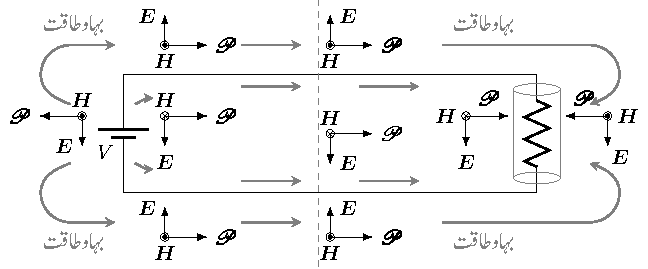
\includegraphics{figWavePoyntingAndCircuitTheory}
\caption{برقی دور میں طاقت کا بہاو۔}
\label{شکل_مستوی_برقی_دور_طاقت_بہاو}
\end{figure}

شکل \حوالہ{شکل_مستوی_برقی_دور_طاقت_بہاو} میں مثبت اور منفی تاروں کے مابین
\begin{align}
V=-\int \kvec{E} \cdot \dif \kvec{l}
\end{align}
برقی دباو پایا جاتا ہے جہاں دو تاروں کے درمیان اس تکمل کو کسی بھی راستے پر حاصل کیا جا سکتا ہے۔برقی میدان \عددی{\kvec{E}} کی سمت مثبت تار سے منفی تار کی  جانب ہے۔اسی طرح تار یا منبع یا مزاحمت کے گرد میدان کا تکمل
\begin{align}
I=\oint \kvec{H} \cdot \dif \kvec{l}
\end{align}
برقی رو دیتا ہے۔شکل میں مختلف مقامات پر \عددی{\kvec{E}} اور \عددی{\kvec{H}} دکھائے گئے ہیں۔ان مقامات پر پوئنٹنگ سمتیہ \عددی{\pmb{\mathscr{P}}=\kvec{E}\times \kvec{H}} بھی دکھائے گئے ہیں۔منبع طاقت پر پوئنٹنگ سمتیہ باہر کی جانب کو ہے جبکہ مزاحمت پر اس کی سمت اندر جانب کو ہے۔منبع طاقت اور مزاحمت کے درمیان نقطہ دار سطح پر پوئنٹنگ سمتیہ منبع سے مزاحمت کی جانب کو ہے۔جگہ جگہ پوئنٹنگ سمتیات دریافت کرتے ہوئے طاقت کے بہاو کو دیکھا جا سکتا ہے۔شکل میں طاقت کے بہاو کو ہلکی سیاہی کے موٹی لکیر سے دکھایا گیا ہے۔

مزاحمت میں منتقل ہوتی طاقت دریافت کرنے کی خاطر مزاحمت کو مکمل گھیرتی ہوئی کسی بھی بند سطح پر پوئنٹنگ سمتیہ کے سطحی تکمل سے حاصل کیا جا سکتا ہے۔شکل میں مزاحمت کے گرد فرضی نلکی ڈبیا دکھائی گئی ہے۔فرض کریں کہ مزاحمت اسی نلکی ڈبیا کے شکل کا ہے۔آئیں اس نلکی ڈبیا کے سطح پر تکمل
\begin{align}
P=\oint (\kvec{E} \times \kvec{H}) \cdot \dif \kvec{S}\quad \quad \text{\RL{اخراجی طاقت}}
\end{align}
حاصل  کریں جو اخراجی طاقت دے گا۔فرض کریں کہ مزاحمت \عددی{z} محدد پر پڑا ہے اور اس کی لمبائی \عددی{L} جبکہ رداس \عددی{a} ہے۔مزاحمت پر \عددی{V} برقی دباو پایا جاتا ہے لہٰذا اس میں میدان \عددی{{\kvec{E}=-\tfrac{V}{L}\az}} ہو گا۔برقی سرحدی شرط کے تحت مزاحمت کے باہر سطح کے قریب برقی میدان یہی ہو گا۔مزاحمت کی گول سطح پر مقناطیسی میدان کو ایمپیئر کے دوری قانون سے حاصل کیا جا سکتا ہے جو \عددی{{\kvec{H}=-\tfrac{I}{2\pi a}\aphi}} برابر حاصل ہوتا ہے۔نلکی ڈبیا کے بالائی اور نچلی ڈھکنوں پر  پوئنٹنگ سمتیہ کا سطحی تکمل صفر کے برابر ہے جبکہ گول سطح پر سطحی تکمل
\begin{align*}
\int\int (\kvec{E} \times \kvec{H}) \cdot \dif \kvec{S}&=\int_{0}^{L} \int_{0}^{2\pi} (\kvec{E}\times \kvec{H} )\cdot (a \dif \phi \dif z \arho)  \\
&=\int_{0}^{L} \int_{0}^{2\pi} -\frac{V I}{2\pi a L} a \dif \phi \dif z \\
&=-V I \quad \quad \quad \quad \quad \text{\RL{اخراجی طاقت}}
\end{align*}
کے برابر ہے۔یوں مزاحمت میں داخل ہوتی طاقت \عددی{P=VI} ہے جو ہمارے توقع کے عین مطابق ہے۔ 

\begin{figure}
\centering
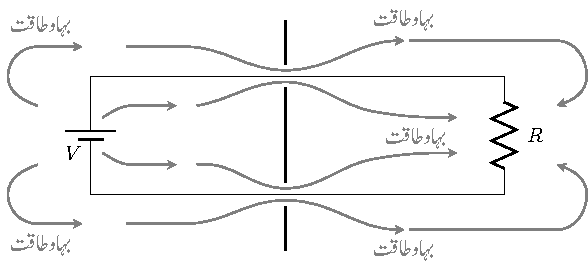
\includegraphics{figWavePoyntingAndCircuitTheoryGroundPlane}
\caption{برقی دور میں زمینی سطح سے طاقتی بہاو پر اثرات۔}
\label{شکل_مستوی_برقی_دور_زمینی_سطح_طاقت_بہاو}
\end{figure}

شکل \حوالہ{شکل_مستوی_برقی_دور_زمینی_سطح_طاقت_بہاو} میں منبع طاقت اور مزاحمت کے درمیان کسی مقام پر لامحدود زمینی سطح نسب کر دی گئی ہے۔اس سطح میں دو باریک سوراخ ہیں جن میں سے برقی تار گزر رہے ہیں۔زمینی سطح پر برقی میدان صفر کے برابر ہوتا ہے لہٰذا زمینی سطح پر پوئنٹنگ سمتیہ صفر کے برابر ہو گا۔یوں اس سطح سے کوئی طاقت نہیں گزر سکتی۔اس شکل میں بھی طاقت کی بہاو دکھائی گئی ہے۔کسی بھی مقام پر پوئنٹنگ سمتیہ کا سطحی تکمل لیتے ہوئے ثابت ہوتا ہے کہ منتقل طاقت کی قیمت جوں کی توں رہتی ہے۔زیادہ دلچسپ صورت حال زمینی سطح میں ان سوراخ پر پائی جاتی ہے۔آپ دیکھیں گے کہ ان سوراخ میں برقی میدان کی قیمت اتنی بڑھ جاتی ہے کہ سوراخ میں سے گزرتی طاقت ہی مزاحمت کو منتقل ہوتی ہے۔ 

آپ نے دیکھا کہ طاقت دراصل برقی تاروں میں سے نہیں گزرتی بلکہ تاروں کے گرد خلاء میں سے گزرتی ہے۔اس عجیب مگر درست نتیجے تک صرف برقی و مقناطیسیت کی مدد سے ہی ہم پہنچ پائیں ہیں۔ 

اگرچہ \عددی{\kvec{E}\times \kvec{H}} عموماً طاقت ہی ظاہر کرتی ہے لیکن یہ ممکن ہے کہ ایسا نہ ہو۔مثلاً اگر زمینی مقناطیسی میدان \عددی{\kvec{H}} اور ساکن چارج کی برقی میدان \عددی{\kvec{E}} کو لیا جائے \عددی{\kvec{E}\times \kvec{H}} سے ایسا ظاہر ہوتا ہے جیسے طاقت کا بہاو پایا جاتا ہے جبکہ ایسا ہرگز درست نہیں ہے۔پوئنٹنگ سمتیہ کے صحیح استعمال کے لئے ضروری ہے کہ جن مقناطیسی اور برقی میدان کی بات کی جائے، وہ دونوں آپس میں تعلق رکھتے ہوں۔ایسے تعلق رکھنے والے میدان کی صورت میں پوئنٹنگ  سمتیہ ہر صورت طاقت کے بہاو کو ظاہر کرے گی۔ 
%========================
\حصہ{موصل میں امواج}
موصل میں امواج پر غور کی خاطر ہم تصور کرتے ہیں کہ موصل سے جڑے ذو برق میں امواج پیدا کئے جاتے ہیں۔ہم جاننا چاہتے ہیں کہ ایسے موج ذو برق اور موصل کے سرحد پر موصل میں کیسے داخل ہوتے ہیں اور موصل میں ان کی کیا کارکردگی ہوتی ہے۔

ایصالی اور انتقالی رو کی شرح \عددیء{\tfrac{\sigma}{\omega \epsilon}} کو مماس ضیاع کہتے ہیں۔یوں ناقص موصل کی مماس ضیاع بلند تعدد پر کم ہو گی۔نائیکروم\فرہنگ{نائیکروم}\حاشیہب{nichrome}\فرہنگ{nichrome} ناقص موصل ہے جس کا مماس ضیاع \عددیء{\SI{100}{\mega\hertz}} تعدد پر  تقریباً \عددیء{\num{2e8}} ہے۔یوں کسی بھی موصل کے لئے \عددیء{\tfrac{\sigma}{\omega \epsilon} \gg 1} ہوتا ہے۔اس حقیقت کو مد نظر رکھتے ہوئے چند سادہ مساوات حاصل کرتے ہیں۔حرکی مستقل
\begin{align*}
\gamma=j \omega \sqrt{\mu \epsilon} \sqrt{1-j \frac{\sigma}{\omega \epsilon}}
\end{align*}
کو \عددیء{\tfrac{\sigma}{\omega \epsilon} \gg 1} کی بنا پر
\begin{align*}
\gamma=j \omega \sqrt{\mu \epsilon}\sqrt{-j \frac{\sigma}{\omega \epsilon}}
\end{align*}
یا
\begin{align*}
\gamma=j \sqrt{-j \omega \mu \sigma}
\end{align*}
لکھا جا سکتا ہے۔اب
\begin{align*}
-j = 1\phase{-90^\circ}
\end{align*}
کے برابر ہے جس کا جزر
\begin{align*}
\sqrt{1\phase{-90^\circ}}=1\phase{-45^\circ}=\frac{1}{\sqrt{2}}-j \frac{1}{\sqrt{2}}
\end{align*}
ہے لہٰذا
\begin{align*}
\gamma=j \left(\frac{1}{\sqrt{2}}-j \frac{1}{\sqrt{2}}\right)\sqrt{\omega \mu \sigma}
\end{align*}
یا
\begin{align}
\gamma=\left(j+1 \right)\sqrt{\pi f \mu \sigma}
\end{align}
حاصل ہوتا ہے جس سے
\begin{align}
\alpha=\beta=\sqrt{\pi f \mu \sigma}
\end{align}
ملتا ہے۔

ان معلومات کے بعد کہا جا سکتا ہے کہ کسی بھی \عددیء{\mu}اور \عددیء{\sigma} مستقل رکھنے والے موصل کے \عددیء{\alpha} اور \عددیء{\beta} ہر تعدد پر برابر ہی رہتے ہیں۔ یوں \عددیء{z} سمت میں دوبارہ امواج فرض کرتے ہوئے موصل میں برقی میدان کی موج کو
\begin{align}\label{مساوات_موج_موصل_موج}
E_x=E_0 e^{-z \sqrt{\pi f \mu \sigma}} \cos (\omega t - z \sqrt{\pi f \mu \sigma})
\end{align}
لکھا جا سکتا ہے۔اگر \عددیء{z<0} کامل ذو برق اور \عددیء{z>0} موصل خطے ہوں تب ان کے سرحد \عددیء{z=0} پر برقی سرحدی شرائط کے مطابق متوازی برقی میدان سرحد کے دونوں اطراف پر برابر ہوں گے۔مساوات \حوالہ{مساوات_موج_موصل_موج} کے تحت سرحد پر موصل میں
\begin{align}\label{مساوات_موج_موصل_ذو_برق_سرحد_موج}
E_x=E_0  \cos \omega t \quad  \quad (z=0)
\end{align}
ہو گا اور یوں سرحد پر ذو برق میں بھی برقی میدان یہی ہو گا۔اب اسی حقیقت کو یوں بھی دیکھا جا سکتا ہے کہ سرحد پر ذو برق میں برقی میدان مساوات \حوالہ{مساوات_موج_موصل_ذو_برق_سرحد_موج} دیتا ہے جو موصل میں سرحد پر اسی قیمت کا میدان پیدا کرتا ہے۔ایسا تصور کرنے کا مطلب یہ ہے کہ ہم ذو برق میں میدان کو منبع میدان تصور کرتے ہیں جو موصل میں مساوات \حوالہ{مساوات_موج_موصل_موج} میں دی موج پیدا کر تا ہے۔موصل میں \عددیء{\tfrac{\sigma}{\omega \epsilon}\gg 1} کی بنا پر انتقالی رو کو نظر انداز کرتے ہوئے
\begin{align}
\kvec{J}=\sigma \kvec{E}
\end{align}
لکھا جا سکتا ہے لہٰذا موصل میں ہر نقطے پر کثافت رو اور برقی میدان راہ تناسب کا تعلق رکھتے ہیں اور یوں موصل میں
\begin{align}\label{مساوات_موج_موصل_کثافت_رو_موج}
J_x=\sigma E_0 e^{-z \sqrt{\pi f \mu \sigma}} \cos (\omega t - z \sqrt{\pi f \mu \sigma})
\end{align}
لکھا جا سکتا ہے۔شکل \حوالہ{شکل_موج_گہرائی_جلد_اور_طاقتی_ضیاع} میں \عددیء{J_x} دکھایا گیا ہے جہاں عین سرحد یعنی \عددیء{z=0} پر کثافت رو کے قیمت \عددیء{\sigma E_0} کو \عددیء{J_0} لکھا گیا ہے۔

مساوات \حوالہ{مساوات_موج_موصل_موج} اور مساوات \حوالہ{مساوات_موج_موصل_کثافت_رو_موج} میں بہت معلومات پائی جاتی ہے۔پہلے ان مساوات میں
  \عددیء{e^{z\sqrt{\pi f \mu \sigma}}} جزو پر غور کریں۔سرحد پر اس کی قیمت \عددیء{{e^{0}=1}} کے برابر ہے جو سرحد سے
\begin{align*}
z=\frac{1}{\sqrt{\pi f \mu \sigma}}
\end{align*}
فاصلے پر \عددیء{e^{-1}=0.368} رہ جاتی ہے۔یہ فاصلہ \اصطلاح{گہرائی جلد}\فرہنگ{گہرائی جلد}\حاشیہب{skin depth}\فرہنگ{skin depth} کہلایا اور \عددیء{\delta} سے ظاہر کیا جاتا ہے۔
\begin{align}\label{مساوات_موج_گہرائی_جلد_تعریف}
\delta =\frac{1}{\sqrt{\pi f \mu \sigma}}
\end{align}
برقی رو کا سطحی تہہ تک محدود رہنے کو \اصطلاح{اثر جلد}\فرہنگ{اثر جلد}\فرہنگ{جلد!اثر}\حاشیہب{skin effect}\فرہنگ{skin effect} کہا جاتا ہے۔
یوں موصل میں
\begin{align}\label{مساوات_موج_گہرائی_جلد_کے_تعلق}
\alpha=\beta=\frac{1}{\delta}
\end{align}
ہو گا۔
اسی طرح سرحد سے \عددیء{2\delta} فاصلے پر میدان \عددیء{e^{-2}=0.135} اور  \عددیء{4\delta} فاصلے پر میدان \عددیء{e^{-4}=0.018} یعنی صرف \عددیء{\SI{1.8}{\%}} رہ جائے گا۔

تانبے کی \عددیء{\sigma=\SI{5.8e7}{\siemens\per \meter}} ہے لہٰذا اس میں گہرائی جلد
\begin{align*}
\delta_{\text{تانبہ}}=\frac{1}{\sqrt{\pi \times f  \times 4 \times \pi \times 10^{-7} \times 5.8 \times 10^{7}}}=\frac{0.0661}{\sqrt{f}}
\end{align*}
میٹر کے برابر ہے۔یوں \عددیء{\SI{50}{\hertz}} کا میدان سرحد سے \عددیء{\tfrac{0.0661}{\sqrt{50}}=\SI{9.35}{\milli\meter}} فاصلے پر کم ہو کر صرف \عددیء{0.368} گنا رہ جائے گا۔برقی ادوار میں مزاحمت میں طاقت کا ضیاع رو کے مربع کے راست تناسب ہوتا ہے لہٰذا ہر ایک گہرائی جلد کے فاصلے پر کثافت طاقت \عددیء{0.368^2=0.135} گنا کم ہو گی۔\اصطلاح{خردامواج}\فرہنگ{خردامواج}\فرہنگ{موج!خرد}\حاشیہب{microwave}\فرہنگ{microwave} کے تعدد یعنی \عددیء{\SI{10}{\giga\hertz}} پر گہرائی جلد \عددیء{\SI{0.661}{\micro\meter}} یعنی نظر آنے والے روشنی کے طول کے آٹھویں حصے  کے برابر ہے۔

ان تعدد پر کسی بھی موصل مثلاً تانبے میں سرحد سے چند ہی گہرائی جلد کے فاصلے پر تمام میدان تقریباً صفر کے برابر ہوتے ہیں۔موصل کے سرحد پر پیدا کئے گئے برقی میدان یا کثافت رو، سرحد سے دوری کے ساتھ تیزی سے کم ہوتے ہیں۔ برقی و مقناطیسی طاقت موصل کے اندر نہیں بلکہ اس کے باہر صفر کرتی ہے۔موصل کا کام صرف اتنا ہے کہ یہ ان امواج کو راستہ دکھاتی ہے۔موصل کے سرحد پر پیدا کثافت رو، موصل میں موج کے حرکت کے عمودی سمت میں داخل ہوتی ہے جس سے موصل میں مزاحمتی ضیاع پیدا ہوتا ہے۔یوں موصل بطور راہ گیر  کردار ادا کرتے ہوئے مزاحمتی ضیاع بطور اجرت حاصل کرتا ہے۔  

اگر آپ کسی بجلی گھر میں \عددیء{\SI{50}{\hertz}}  کے برقی رو کو منتقل کرنے کی خاطر پانچ سنٹی میٹر رداس کے تانبے کی ٹھوس تار استعمال کر رہے ہوں تو یہ سراسر تانبہ ضائع کرنا ہو گا چونکہ کثافت رو تار کے بیرونی سطح پر ہی پائی جائے گی۔اندرونی تار، سطح سے دور، کثافت رو قابل نظرانداز ہو گی لہٰذا اس سے بہتر ہو گا کہ زیادہ رداس کی نلکی نما تار استعمال کی جائے جس کی موٹائی تقریباً \عددیء{1.5\delta} یعنی \عددیء{\SI{1.4}{\centi\meter}} ہو۔اگرچہ یہ فیصلہ لامحدود جسامت کے سرحد کے نتائج پر بنیاد ہے، حقیقت میں محدود سرحد پر بھی میدان اسی نسبت سے گھٹتے ہیں۔

بلند تعدد پر گہرائی جلد کا فاصلہ اتنا کم ہوتا ہے کہ راہ گیر موصل کی سطحی تہہ ہی اہمیت رکھتی ہے۔یوں خرد امواج کی منتقلی کے لئے شیشے پر \عددیء{\SI{0.661}{\micro\meter}} موٹی چاندی کی تہہ کافی ہے۔

آئیں اب موصل میں طول موج اور رفتار موج کے مساوات حاصل کریں۔ہم
\begin{align*}
\beta=\frac{2\pi}{\lambda}
\end{align*}
سے شروع کرتے ہوئے مساوات \حوالہ{مساوات_موج_گہرائی_جلد_کے_تعلق} استعمال کرتے ہوئے
\begin{align*}
\lambda=2\pi\delta
\end{align*}
لکھ سکتے ہیں۔اسی طرح مساوات \حوالہ{مساوات_موج_رفتار_اور_تعدد}
\begin{align*}
v=\frac{\omega}{\beta}
\end{align*}
سے
\begin{align}
v=\omega \delta
\end{align}
ملتا ہے۔

تانبے میں \عددیء{\SI{50}{\hertz}} پر \عددیء{\lambda=\SI{5.8}{\centi\meter}} اور \عددیء{v=\SI{2.94}{\meter\per\second}} یا \عددیء{\SI{10.6}{\kilo\meter\per\hour}} حاصل ہوتے ہیں۔میں تقریباً \عددیء{\SI{6}{\kilo \meter\per\hour}} کی رفتار سے چلتا ہوں۔یوں آپ دیکھ سکتے ہیں کہ تانبے میں برقی و مقناطیسی امواج انتہائی آہستہ چلتے ہیں۔یاد رہے کہ اسی \عددیء{\SI{50}{\hertz}} کے موج کی خالی خلاء میں \عددیء{\lambda=\SI{6000}{\kilo\meter}} اور  رفتار \عددیء{\SI{3e8}{\meter\per\second}} ہو گی۔

موصل میں \عددیء{H_y} کی مساوات لکھنے کی خاطر موصل کی قدرتی رکاوٹ درکار ہو گی۔مساوات \حوالہ{مساوات-موج_قدرتی_رکاوٹ}
\begin{align*}
\eta =\sqrt{\frac{j \omega \mu}{\sigma +j \omega \epsilon}}
\end{align*}
کو \عددیء{\tfrac{\sigma}{\omega \epsilon}\gg1} کی وجہ سے
\begin{align*}
\eta=\sqrt{\frac{j\omega\mu}{\sigma}}
\end{align*}
یا
\begin{align}\label{مساوات_موج_قدرتی_رکاوٹ_موصل_گہرائی_جلد_کے_ساتھ}
\eta=\frac{\sqrt{2}\phase{45^\circ}}{\sigma \delta}=\frac{1}{\sigma \delta}+j\frac{1}{\sigma \delta}
\end{align}
لکھا جا سکتا ہے۔یوں مساوات \حوالہ{مساوات_موج_موصل_ذو_برق_سرحد_موج} کو گہرائی جلد کی صورت
\begin{align}
E_x=E_0 e^{-\frac{z}{\delta}} \cos \left(\omega t -\frac{z}{\delta}\right)
\end{align}
 میں لکھتے ہوئے مقناطیسی موج کو
\begin{align}
H_y=\frac{\sigma \delta E_0}{\sqrt{2}} e^{-\frac{z}{\delta}} \cos \left(\omega t-\frac{z}{\delta}-\frac{\pi}{4}\right)
\end{align}
لکھا جا سکتا ہے جہاں سے آپ دیکھ سکتے ہیں کہ مقناطیسی موج، برقی موج سے  پھیرے کے آٹھویں حصے پیچھے ہے۔

مندرجہ بالا دو مساوات کی مدد سے پوئنٹنگ مساوات
 \begin{align*}
\mathscr{P}_{\text{اوسط}}=\frac{1}{2} \frac{\sigma \delta E_0^2}{\sqrt{2}} e^{-\frac{2 z}{\delta}} \cos \frac{\pi}{4}
\end{align*}
یا
\begin{align*}
\mathscr{P}_{\text{اوسط}}=\frac{\sigma \delta E_0^2}{4} e^{-\frac{2 z}{\delta}}
\end{align*}
دیتا ہے۔ آپ دوبارہ دیکھ سکتے ہیں کہ ایک گہرائی جلد کی گہرائی پر کثافت طاقت، سرحد کے کثافت طاقت کے \عددیء{e^{-2}=0.135} گنا رہ گئی ہے۔

\begin{figure}
\centering
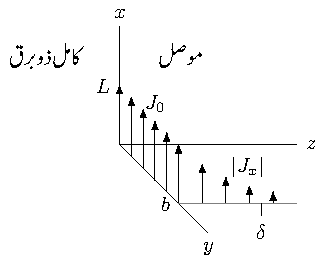
\includegraphics{figWaveSkinDepthLoss}
\caption{موصل میں طاقت کے ضیاع اور گہرائی جلد۔}
\label{شکل_موج_گہرائی_جلد_اور_طاقتی_ضیاع}
\end{figure}

شکل \حوالہ{شکل_موج_گہرائی_جلد_اور_طاقتی_ضیاع} پر دوبارہ نظر ڈالیں۔مسئلہ پوئنٹنگ کہتا ہے کہ سرحد پر \عددیء{L} اور \عددیء{b} اطراف کے مستطیل میں جتنی برقی و مقناطیسی طاقت داخل ہوتی ہے، وہ تمام کی تمام موصل میں ضائع ہو جاتی ہے۔یہ طاقت
\begin{align*}
P_{L,\text{اوسط}}&=\int_0^b \int_0^L \left. \mathscr{P}_{\text{اوسط}}\right|_{z=0} \dif x \dif y\\
&=\int_0^b \int_0^L \left. \frac{\sigma \delta E_0^2}{4} e^{-\frac{2 z}{\delta}}\right|_{z=0} \dif x \dif y\\
&=\frac{\sigma \delta b L E_0^2}{4}
\end{align*}
کے برابر ہے۔سرحدی کثافت رو
\begin{align*}
J_0=\sigma E_0
\end{align*}
کی صورت میں اسے
\begin{align}\label{مساوات_موج_اوسط_مزاحمتی_ضیاع_الف}
P_{L,\text{اوسط}}&=\frac{1}{4\sigma} \delta b L J_0^2
\end{align}
لکھا جا سکتا ہے۔

آئیں دیکھیں کہ اگر \عددیء{b} چوڑائی میں کل برقی رو کو \عددیء{\delta} گہرائی تک محدود کر دیا جائے تو مزاحمتی ضیاع کتنا ہو گا۔ایسا کرنے کی خاطر پہلے اس چوڑائی میں کل رو
\begin{align*}
I=\int_0^{\infty}\int_0^b J_x \dif y \dif z
\end{align*}
حاصل کرتے ہیں جہاں تکمل آسان بنانے کی غرض سے
\begin{align*}
J_x=J_0 e^{-\frac{z}{\delta}} \cos \left(\omega t -\frac{z}{\delta}\right)
\end{align*}
کو دوری سمتیہ کی شکل
\begin{align*}
J_{xs}&=J_0 e^{-\frac{z}{\delta}}e^{-j\frac{z}{\delta}}\\
&=J_0 e^{-(1+j)\frac{z}{\delta}}
\end{align*}
میں لکھ کر تکمل حل کرتے ہیں۔
\begin{align*}
I&=\int_0^{\infty}\int_0^bJ_0 e^{-(1+j)\frac{z}{\delta}} \dif y \dif z\\
&=\frac{J_0 b \delta}{1+j}
\end{align*}
اس سے
\begin{align*}
I=\frac{J_0 b \delta}{\sqrt{2}} \cos \left(\omega t - \frac{\pi}{4} \right)
\end{align*}
لکھا جائے گا۔اگر اس رو کو \عددیء{0<y<b} اور \عددیء{0<z<\delta} میں محدود کر دیا جائے تب نئی کثافت رو
\begin{align*}
J_x'=\frac{J_0}{\sqrt{2}} \cos \left(\omega t - \frac{\pi}{4} \right)
\end{align*}
ہو گی۔مزاحمتی طاقت کا ضیاع فی اکائی حجم \عددیء{\kvec{J} \cdot \kvec{E}} کے برابر ہے لہٰذا اس حجم میں کل ضیاع
\begin{align*}
P_L=\frac{1}{\sigma}\left(J_x'\right)^2 b L \delta=\frac{J_0^2}{2\sigma} b L \delta \cos^2 \left(\omega t -\frac{\pi}{4} \right)
\end{align*}
ہو گا۔مربع کوسائن موج کی اوسط قیمت \عددیء{\tfrac{1}{2}} کے برابر ہوتی ہے لہٰذا اوسط طاقت کے ضیاع کو
\begin{align}
P_L=\frac{J_0^2 b L \delta}{4\sigma}
\end{align}
لکھا جا سکتا ہے جو عین مساوات \حوالہ{مساوات_موج_اوسط_مزاحمتی_ضیاع_الف} ہے۔

اس نتیجے کو دیکھ کر اب کسی بھی موصل، جس میں اثر جلد پایا جاتا ہو، میں کل رو کو ایک جلد گہرائی میں یکساں تقسیم شدہ تصور کرتے ہوئے سلاخ کی مزاحمتی ضیاع حاصل کی جا سکتی  ہے۔یوں  \عددیء{b} چوڑائی، \عددیء{L} لمبائی اور لامحدود گہرائی سلاخ جس میں اثر جلد پایا جاتا ہو اور \عددیء{b} چوڑائی، \عددیء{L} لمبائی اور \عددیء{\delta}  گہرائی سلاخ جس میں یکساں تقسیم شدہ رو ہو کے مزاحمت بالکل برابر ہوں گے۔

اس حقیقت کو استعمال کرتے ہوئے رداس \عددیء{r} کے  ٹھوس نلکی سلاخ کی مزاحمت بلند تعدد پر حاصل کی جا سکتی ہے۔اگر گہرائی جلد سلاخ کے رداس سے بہت کم ہو تب اس طرح حاصل کردہ مزاحمت کی قیمت تقریباً بالکل درست ہو گی۔ایسی تعدد جس پر اثر جلد پایا جاتا ہو کی صورت میں سلاخ کی بیرونی جلد ہی رو گزارے گی لہٰذا مزاحمت کی قیمت حاصل کرتے وقت اس نلکی نما جھلی کو ہی موصل تصور کیا جائے گا لہٰذا مزاحمت \عددیء{R}
\begin{align}
R=\frac{L}{\sigma S}=\frac{L}{\sigma 2 \pi r \delta}
\end{align}

ایک ملی میٹر رداس اور دس میٹر لمبی تانبے کے تار کی یک سمتی مزاحمت
\begin{align*}
R_{\text{\RL{یک سمتی}}}=\frac{10}{5.8\times 10^7 \times \pi \times 0.001^2}=\SI{54.88}{\milli \ohm}
\end{align*}
ہے۔ ایک سو میگا ہرٹز کی تعدد پر تانبے کی \عددیء{\delta=\SI{6.61}{\micro\meter}} ہو گی لہٰذا اس تعدد پر اسی تار کی مزاحمت
\begin{align*}
R=\frac{10}{5.8 \times 10^7 \times 2\times \pi \times 0.001 \times 6.61 \times 10^{-6} }=\SI{4.15}{\ohm}
\end{align*}
ہو گی۔
%=============================
\ابتدا{مشق}
ٹھوس نلکی نما لوہے کی تار جس کا رداس \عددیء{\SI{5}{\milli \meter}} اور جس کی لمبائی \عددیء{\SI{2.5}{\meter}} ہے میں \عددیء{2\cos 10000 t} ایمپیئر کی برقی رو گزر رہی ہے۔کتاب کے آخر میں ضمیمے سے \عددیء{\sigma=\SI{1.03e7}{\siemens \per \meter}} اور \عددیء{\mu_R=4000} دئے گئے ہیں۔یاد رہے کہ موصل کا \عددیء{\epsilon_R=1} ہوتا ہے۔ آپ سے گزارش ہے کہ مندرجہ ذیل حاصل کریں۔

\begin{itemize}
\item
یک سمتی رو مزاحمت،
\item
گہرائی جلد،
\item
بدلتی رو مزاحمت یا موثر مزاحمت،
\item
مزاحمتی طاقت کا ضیاع۔
\end{itemize}

جوابات: \عددیء{\SI{3.09}{\milli \ohm}}، \عددیء{\SI{62}{\micro\meter}}، \عددیء{\SI{1.25}{\ohm}} اور \عددیء{\SI{2.49}{\watt}}
\انتہا{مشق}
%=============================

\حصہ{انعکاس مستوی موج}
لامحدود جسامت کے حجم میں مستوی امواج ہم دیکھ چکے۔ایسے حجم میں کبھی بھی موج دو مختلف اقسام کے اشیاء کے درمیان پائی جانے والی سرحد نہیں چھوتی۔آئیں محدود جسامت کے حجم میں مستوی امواج پر غور کریں جہاں امواج کو ایک قسم کے مادے سے دوسرے قسم کے مادے میں داخل ہونا ہو گا۔آپ دیکھیں گے کہ ایسی صورت میں موج کا کچھ حصہ پہلے خطے سے دوسرے خطے میں داخل ہو پاتا ہے جبکہ اس کا بقایا حصہ سرحد سے ٹکرا کر واپس پہلے خطے میں لوٹ جاتا ہے۔اس حصے میں ہم سرحد سے گزرتے اور اس سے ٹکرا کر واپس لوٹتے حصوں کے مساوات حاصل کریں گے۔یہ نتائج \اصطلاح{ترسیلی تاروں}\حاشیہب{transmission lines}  اور  \اصطلاح{رہبر موج}\حاشیہب{waveguide} کے مسائل میں جوں کے توں قابل استعمال ہوں گے۔
\begin{figure}
\centering
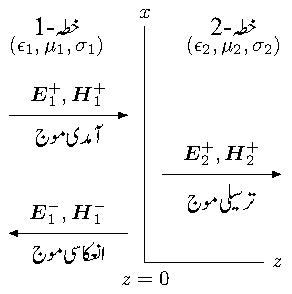
\includegraphics{figWaveReflectionNormalIncidence}
\caption{آمدی موج سرحد سے گزرتی ترسیلی اور اس سے  لوٹتی انعکاسی امواج پیدا کرتی ہے۔}
\label{شکل_موج_آمدی_انعکاسی_ترسیلی}
\end{figure}

ہم \عددیء{z<0} کو خطہ-1 تصور کرتے ہیں جہاں \عددیء{(\epsilon_1,\mu_1,\sigma_1)} ہیں جبکہ \عددیء{z>0} کو خطہ-2 تصور کرتے ہیں جہاں \عددیء{(\epsilon_2,\mu_2,\sigma_2)} ہیں۔یہ صورت حال شکل \حوالہ{شکل_موج_آمدی_انعکاسی_ترسیلی} میں دکھائی گئی ہے۔ہم بڑھتے \عددیء{z} جانب حرکت کرتے موج کو بالانوشت \عددیء{+} جبکہ گھٹتے \عددیء{z} جانب حرکت کرتے موج کو بالانوشت \عددیء{-} سے ظاہر کریں گے۔اب تصور کریں کہ پہلے خطے میں سرحد کی جانب برقی موج
\begin{align}\label{مساوات_موج_برقی_الف_آمد}
E_{xs1}^+=E_{x10}^+e^{-\gamma_1 z}
\end{align}
آتی ہے۔آپ جانتے ہیں کہ اس برقی موج کے ساتھ لازماً مقناطیسی موج
\begin{align}
H_{ys1}^+=\frac{E_{x10}^+}{\eta_1} e^{-\gamma_1 z}\label{مساوات_موج_مقناطیسی_الف_آمد}
\end{align}
بھی ہو گی۔ سرحد کی طرف آتے موج کو \اصطلاح{آمدی موج}\فرہنگ{آمدی موج}\فرہنگ{موج!آمدی}\حاشیہب{incident wave}\فرہنگ{incident wave} کہا جاتا ہے۔چونکہ یہ موج سرحد کے عمودی حرکت کر رہا ہے لہٰذا اس کے حرکت کو \اصطلاح{عمودی آمد}\فرہنگ{عمودی آمد}\فرہنگ{موج!عمودی آمد}\حاشیہب{normal incidence}\فرہنگ{normal incidence} کہتے ہیں۔

اس آمدی موج کا کچھ حصہ جسے \اصطلاح{ترسیلی موج}\فرہنگ{ترسیلی موج}\فرہنگ{موج!ترسیلی}\حاشیہب{transmitted wave}\فرہنگ{transmitted wave} کہتے ہیں، سرحد سے گزرتے ہوئے  سیدھا چلے جائے گا۔ترسیلی امواج
\begin{align}
E_{xs2}^+&=E_{x20}^+e^{-\gamma_2 z}\label{مساوات_موج_برقی_ب_ترسیلی}\\
H_{ys2}^+&=\frac{E_{x20}^+}{\eta_2} e^{-\gamma_2 z}\label{مساوات_موج_مقناطیسی_ب_ترسیلی}
\end{align}
ہیں۔سرحد کے دوسرے جانب حرکی مستقل \عددیء{\gamma_2} اور قدرتی رکاوٹ \عددیء{\eta_2} ہیں جو پہلے خطے سے مختلف ہیں۔ترسیلی امواج سرحد سے دور چلتی جاتی ہیں۔

آمدی اور ترسیلی برقی امواج \عددیء{x} محدد کے متوازی جبکہ مقناطیسی امواج \عددیء{y} محدد کے متوازی ہیں لہٰذا یہ چاروں امواج سرحد کے بھی متوازی ہیں۔صفحہ \حوالہصفحہ{مساوات_میکس_ویل_سرحدی_شرائط_بدلتے_میدان_الف} پر مساوات \حوالہ{مساوات_میکس_ویل_سرحدی_شرائط_بدلتے_میدان_الف} اور اس کے قریب ہی مساوات \حوالہ{مساوات_میکس_ویل_متوازی_مقناطیسی_موج_سرحدی_شرط} متوازی امواج کے سرحدی شرائط بیان کرتے ہیں۔اب کائنات میں کبھی بھی دو اشیاء کے سرحد پر سطحی کثافت رو نہیں پائی جاتی۔یوں \عددیء{K_\perp=0} لیتے ہوئے ان شرائط کو
\begin{align*}
E_{m1}&=E_{m2}\\
H_{m1}&=H_{m2} \quad(K_\perp=0)
\end{align*}
لکھا جاتا ہے۔

اب اگر پہلی شرط پوری کی جائے تو سرحد کے دونوں اطراف پر متوازی برقی میدان برابر ہوں گے  لہٰذا \عددیء{z=0} پر مساوات \حوالہ{مساوات_موج_برقی_الف_آمد} اور مساوات \حوالہ{مساوات_موج_برقی_ب_ترسیلی} برابر ہوں گے۔یوں \عددیء{E_{x10}^+=E_{x20}^+} حاصل ہوتا ہے لیکن دوسری شرط کے مطابق سرحد کے دونوں جانب متوازی مقناطیسی میدان بھی برابر ہونا ہو گا لہٰذا \عددیء{z=0} پر مساوات \حوالہ{مساوات_موج_مقناطیسی_الف_آمد} اور مساوات \حوالہ{مساوات_موج_مقناطیسی_ب_ترسیلی} بھی برابر ہوں گے جس سے \عددیء{\frac{E_{x10}^+}{\eta_1}=\frac{E_{x20}^+}{\eta_2}} حاصل ہوتا ہے۔یہ دونوں تب ممکن ہے جب \عددیء{\eta_1=\eta_2} ہو جو حقیقت میں کبھی بھی نہیں ہو گا لہٰذا صرف آمدی اور ترسیلی امواج کی صورت میں سرحدی شرائط پر پورا نہیں اترا جا سکتا۔مندرجہ بالا دونوں سرحدی شرائط صرف اس صورت میں پورا ہوتے ہیں جب سرحد سے ٹکرا کر واپس لوٹتے امواج
\begin{align}
E_{xs1}^-&=E_{x10}^-e^{\gamma_1 z}\\
H_{ys1}^-&=-\frac{E_{x10}^-}{\eta_1} e^{\gamma_1 z}
\end{align}
 بھی پائے جائیں جنہیں \اصطلاح{انعکاسی امواج}\فرہنگ{انعکاسی امواج}\فرہنگ{موج!انعکاسی}\حاشیہب{reflected wave}\فرہنگ{reflected wave} کہا جاتا ہے۔انعکاسی موج کا  حرکی مستقل \عددیء{\gamma_1} ہی ہے جبکہ یہ موج  گھٹتے \عددیء{z} جانب حرکت کر رہی ہے۔انعکاسی موج میں \عددیء{E_{x10}^-} مخلوط عدد ہو سکتا ہے۔چونکہ انعکاسی امواج گھٹتے \عددیء{z} جانب حرکت کرتی ہیں لہٰذا مسئلہ پوئنٹنگ کے تحت \عددیء{E_{xs1}^-=-\eta_1H_{ys1}^-} ہو گا تا کہ \عددیء{{\kvec{E}_1^- \times \kvec{H}_1^-}} کی سمت \عددیء{-\az} ہو۔

آمدی، ترسیلی اور انعکاسی امواج کی صورت میں دونوں سرحدی شرائط پورے ہوتے ہیں اور ان کی مدد سے \عددیء{E_{x10}^+} کی صورت میں بقایا تمام امواج کے طول بھی حاصل ہوتے ہیں۔آئیں دیکھیں کہ ایسا کس طرح ہوتا ہے۔

اب پہلے خطے میں آمدی امواج کے علاوہ انعکاسی امواج بھی پائے جاتے ہیں لہٰذا سرحدی شرائط میں دونوں کا مجموعہ استعمال کیا جائے گا۔یوں \عددیء{z=0} پر سرحد کے دونوں جانب متوازی برقی میدان برابر  ہونے سے
\begin{align*}
E_{xs1}=E_{xs2}    \quad (z=0)
\end{align*}
یعنی
\begin{align*}
E_{xs1}^+ +E_{xs1}^-=E_{xs2}^+ \quad (z=0)
\end{align*}
یا
\begin{align}\label{مساوات_موج_برقی_شرط_پورا}
E_{x10}^+ + E_{x10}^-&=E_{x20}^+
\end{align}
حاصل ہوتا ہے۔اسی طرح  \عددیء{z=0} پر سرحد کے دونوں جانب متوازی مقناطیسی میدان کے برابری سے
\begin{align*}
H_{ys1}=H_{ys2} \quad (z=0, K_\perp=0)
\end{align*}
یعنی
\begin{align*}
H_{ys1}^+ +H_{ys1}^-=H_{ys2}^+ \quad (z=0, K_\perp=0)
\end{align*}
یا
\begin{align}\label{مساوات_موج_مقناطیسی_شرط_پورا}
\frac{E_{x10}^+}{\eta_1}-\frac{E_{x10}^-}{\eta_1}=\frac{E_{x20}^+}{\eta_2}
\end{align}
حاصل ہوتا ہے۔مساوات \حوالہ{مساوات_موج_برقی_شرط_پورا} اور مساوات \حوالہ{مساوات_موج_مقناطیسی_شرط_پورا} کو \عددیء{E_{x10}^-} کی خاطر حل کرنے کی غرض سے مساوات \حوالہ{مساوات_موج_برقی_شرط_پورا} کو مساوات \عددیء{مساوات_موج_مقناطیسی_شرط_پورا} میں پر کرتے
\begin{align*}
\frac{E_{x10}^+}{\eta_1}-\frac{E_{x10}^-}{\eta_1}=\frac{E_{x10}^+ + E_{x10}^-}{\eta_2}
\end{align*}
ہوئے یوں
\begin{align*}
E_{x10}^- =E_{x10}^+ \frac{\eta_2-\eta_1}{\eta_2+\eta_1}
\end{align*}
حاصل ہوتا ہے۔انعکاسی اور آمدی برقی میدان کے حیطوں کی شرح کو \اصطلاح{شرح انعکاس}\فرہنگ{شرح!انعکاس}\حاشیہب{reflection coefficient}\فرہنگ{reflection coefficient} پکارا  اور \عددیء{\Gamma} سے ظاہر\حاشیہد{\عددیء{\Gamma} یونانی حروف تہجی گیما ہے۔} کیا جاتا ہے۔
\begin{align}\label{مساوات_موج_شرح_انعکاس_تعریف}
\Gamma=\frac{E_{x10}^-}{E_{x10}^+}=\frac{\eta_2-\eta_1}{\eta_2+\eta_1}
\end{align}
مخلوط شرح انعکاس کی صورت میں انعکاسی اور آمدی میدان میں زاویائی فرق پایا جائے گا۔آپ دیکھ سکتے ہیں کہ شرح انعکاس کی حتمی قیمت صفر تا ایک ممکن ہے۔
\begin{align}
\abs{\Gamma} \le 1
\end{align}

اسی طرح مساوات \حوالہ{مساوات_موج_برقی_شرط_پورا} اور مساوات \حوالہ{مساوات_موج_مقناطیسی_شرط_پورا} سے \عددیء{E_{x10}^-} ختم کرنے سے
\begin{align}\label{مساوات_موج_شرح_ترسیل_تعریف}
\tau=\frac{E_{x20}^+}{E_{x10}^+ }=\frac{2\eta_2}{\eta_2+\eta_1}
\end{align}
حاصل ہوتا ہے جو  \اصطلاح{شرح ترسیل}\فرہنگ{شرح ترسیل}\حاشیہب{transmission coefficient}\فرہنگ{transmission coefficient} کہلایا اور \عددیء{\tau} سے ظاہر کیا جاتا ہے۔مساوات \حوالہ{مساوات_موج_شرح_انعکاس_تعریف} اور مساوات \حوالہ{مساوات_موج_شرح_ترسیل_تعریف} سے
\begin{align}
\tau=1+\Gamma
\end{align}
لکھا جا سکتا ہے۔

آئیں ان نتائج کو چند مخصوص صورتوں میں استعمال کرتے ہیں۔تصور کریں کہ پہلا خطہ کامل ذو برق جبکہ دوسرا خطہ کامل موصل ہے۔ایسی صورت میں \عددیء{\sigma_2} لامحدود ہو گا لہٰذا
\begin{align*}
\eta_2=\sqrt{\frac{j \omega \mu_2}{\sigma_2+j\omega \epsilon_2}}=0
\end{align*} 
ہو گا۔یوں مساوات \حوالہ{مساوات_موج_شرح_ترسیل_تعریف} سے 
\begin{align*}
E_{x20}^+=0
\end{align*}
حاصل ہوتا ہے یعنی کامل موصل میں کسی صورت بھی وقت کے ساتھ بدلتا میدان نہیں پایا جا سکتا۔اس کو یوں بھی بیان کیا جا سکتا ہے کہ کامل موصل کی گہرائی جلد صفر کے برابر ہے۔

مساوات \حوالہ{مساوات_موج_شرح_انعکاس_تعریف} میں \عددیء{\eta_2=0} پر کرنے سے
\begin{align*}
\Gamma=-1
\end{align*}
یعنی
\begin{align*}
E_{x10}^-=-E_{x10}^+
\end{align*}
حاصل ہوتا ہے۔انعکاسی موج کا حیطہ بالکل آمدی موج کے حیطے کے برابر ہے لیکن ان میں \عددیء{180^\circ} کا زاویہ پایا جاتا ہے۔موصل سطح آمدی توانائی کو واپس کرتی ہے اور یوں پہلے خطے میں کل برقی میدان
\begin{align*}
E_{xs1}&=E_{xs1}^+ +E_{xs1}^-\\
&=E_{x10}^+ e^{-j \beta_1 z}-E_{x10}^+ e^{j \beta_1 z}
\end{align*}
ہو گا جہاں کامل ذو برق میں \عددیء{\gamma_1=0+j\beta_1} لیا گیا ہے۔اس کو حل کرتے ہوئے
\begin{align*}
E_{xs1}&=E_{x10}^+ \left(e^{-j \beta_1 z}-e^{j\beta_1 z} \right)\\
&=-j 2 E_{x10}^+ \sin \beta_1 z
\end{align*}
حاصل ہوتا ہے جو دوری سمتیہ کی صورت میں ہے جسے \عددیء{e^{j \omega t}} سے ضرب دے کر حقیقی جزو لیتے ہوئے اصل موج کی مساوات
\begin{align}\label{مساوات_موج_دو_امواج_برابر_ساکن_موج}
E_{x1}=2 E_{x10}^+ \sin \beta_1 z \sin \omega t
\end{align}
حاصل ہوتی ہے۔یہ مساوات ساکن میدان کو ظاہر کرتی ہے۔یاد رہے کہ اسے دو آپس میں الٹ سمت میں حرکت کرتے امواج سے حاصل کیا گیا ہے۔اس کا موازنہ آمدی موج
\begin{align*}
E_{x1}^+=E_{x10}^+ \cos (\omega t - \beta_1 z)
\end{align*}
سے کریں۔حرکت کرتے موج کی پہچان جزو \عددیء{\omega t -\beta_1 z} ہے جو مثبت سمت میں موج کو ظاہر کرتی ہے۔مساوات \حوالہ{مساوات_موج_دو_امواج_برابر_ساکن_موج} میں \عددیء{\omega t} اور \عددیء{\beta_1 z} علیحدہ علیحدہ پائے جاتے ہیں۔

مساوات \حوالہ{مساوات_موج_دو_امواج_برابر_ساکن_موج} میں جس لمحہ \عددیء{\omega t =n\pi} کے برابر ہو اس لمحہ میدان ہر نقطے پر صفر کے برابر ہو گا۔اس کے علاوہ جس نقطے پر  \عددیء{\beta_1 z=n\pi} کے برابر ہو، اس نقطے پر ہر وقت میدان صفر ہی رہتا ہے۔مساوات \حوالہ{مساوات_موج_دو_امواج_برابر_ساکن_موج} کو \اصطلاح{ساکن موج}\فرہنگ{ساکن موج}\فرہنگ{موج!ساکن}\حاشیہب{standing wave}\فرہنگ{standing wave} کہا جاتا ہے۔برقی میدان ان سطحوں پر ہر وقت صفر رہتا ہے جہاں
\begin{align*}
\beta_1 z = n\pi \quad (n=0,\mp 1, \mp 2, \cdots)
\end{align*}
ہو جس سے
\begin{align*}
\frac{2\pi}{\lambda_1} z =n \pi
\end{align*}
یعنی
\begin{align*}
z=n\frac{\lambda_1}{2}
\end{align*}
حاصل ہوتا ہے۔یوں سرحد یعنی \عددیء{z=0} پر برقی میدان صفر ہو گا اور پہلے خطے میں سرحد سے دور چلتے ہوئے ہر آدھے  طول موج پر صفر برقی میدان پایا جائے گا۔یہ صورت حال شکل \حوالہ{شکل_موج_ساکن_برقی_موج} میں دکھائی گئی ہے۔اس شکل میں نقطہ دار لکیر ان سطحوں کو ظاہر کرتی ہیں جہاں میدان صفر رہتا ہے۔برقی میدان کو وقت \عددیء{t=\tfrac{\pi}{2}} پر دکھایا گیا ہے جب اس کا حیطہ زیادہ سے زیادہ ہوتا ہے۔ 

\begin{figure}
\centering
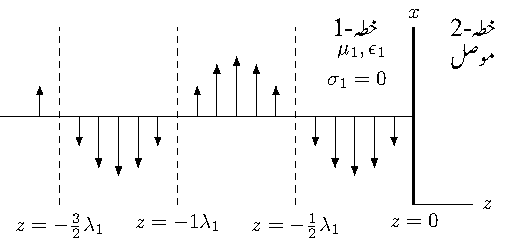
\includegraphics{figWaveStandingWave}
\caption{ساکن موج، برقی میدان۔}
\label{شکل_موج_ساکن_برقی_موج}
\end{figure}

چونکہ \عددیء{E_{xs1}^+=\eta_1 H_{ys1}^+} اور \عددیء{E_{xs1}^-=-\eta_1 H_{ys1}^-} ہوتے ہیں لہٰذا مقناطیسی میدان
\begin{align*}
H_{ys1}=\frac{E_{x10}^+}{\eta_1} \left(e^{-j\beta_1 z}+e^{j \beta_1 z} \right)
\end{align*}
یا
\begin{align}
H_{y1}=2 \frac{E_{x10}^+}{\eta_1} \cos \beta_1 z \cos \omega t
\end{align}
ہو گا۔یہ بھی ساکن موج ہے لیکن  جس سطح پر  برقی میدان صفر رہتا ہے وہاں مقناطیسی ساکن موج کی چوٹی پائی جاتی ہے۔اس کے علاوہ برقی اور مقناطیسی ساکن امواج میں \عددیء{90^\circ} کا وقتی فرق پایا جاتا ہے لہٰذا یہ امواج کسی بھی سمت میں اوسطاً صفر طاقت منتقل کرتی ہیں۔

آئیں اب دو کامل ذو برق کی سرحد پر صورت حال دیکھیں۔اب ان دو خطوں میں قدرتی رکاوٹ \عددیء{\eta_1} اور \عددیء{\eta_2} جبکہ \عددیء{\alpha_1=0} اور \عددیء{\alpha_2=0} ہوں گے۔عددی قیمتیں لے کر آگے چلتے ہیں۔فرض کریں کہ
\begin{align*}
\eta_1&=\SI{50}{\ohm}\\
\eta_2&=\SI{377}{\ohm}\\
E_{x10}^+&=\SI{10}{\volt \per \meter}
\end{align*}
ہیں۔یوں
\begin{align*}
\Gamma=\frac{377-50}{377+50}=0.7658
\end{align*}
ہے لہٰذا
\begin{align*}
E_{x10}^-=0.7658 \times 10=\SI{7.658}{\volt \per \meter}
\end{align*}
ہو گا۔پہلے خطے میں مقناطیسی میدان
\begin{align*}
H_{y10}^+&=\frac{10}{50}=\SI{0.2}{\ampere \per \meter}\\
H_{y10}^-&=-\frac{7.658}{50}=\SI{-0.153}{\ampere\per\meter}
\end{align*}
ہیں۔آمدی اوسط سطحی کثافت طاقت مساوات \حوالہ{مساوات_موج_پوئنٹنگ_مسئلہ} سے
\begin{align*}
P_{1,\text{اوسط}}^+=\frac{1}{2}  \frac{\left(E_{x10}^+\right)^2}{\abs{\eta_1}} e^{-2 \alpha_1 z} \cos \theta_{\eta 1}=\SI{1}{\watt \per \meter \squared}
\end{align*}
جبکہ انعکاسی اوسط سطحی کثافت طاقت
\begin{align*}
P_{1,\text{اوسط}}^-=\frac{1}{2}  \frac{\left(E_{x10}^-\right)^2}{\abs{\eta_1}} e^{-2 \alpha_1 z} \cos \theta_{\eta 1}=\SI{0.5864}{\watt \per \meter \squared}
\end{align*}
ہے۔ان مساوات میں \عددیء{\alpha_1=0} اور \عددیء{\eta_1=50\phase{0}} استعمال کئے گئے۔آپ دیکھ سکتے ہیں کہ انعکاسی اور آمدی کثافت طاقت کی شرح
\begin{align}
\frac{\frac{\left(E_{x10}^-\right)^2}{2\eta_0}}{\frac{\left(E_{x10}^+\right)^2}{2\eta_0}} =\abs{\Gamma}^2
\end{align}
کے برابر ہے۔

 دوسرے خطے میں
\begin{align*}
E_{x20}^+&=\frac{2\eta_2}{\eta_2+\eta_1} E_{x10}^+=\SI{17.658}{\volt \per \meter}\\
H_{y20}^+&=\frac{17.658}{377}=\SI{0.04684}{\ampere\per\meter}
\end{align*}
ہیں لہٰذا
\begin{align*}
P_{2,\text{اوسط}}^+=\frac{1}{2}  \frac{\left(E_{x20}^+\right)^2}{\abs{\eta_2}} e^{-2 \alpha_2 z} \cos \theta_{\eta 2}=\SI{0.4135}{\watt \per \meter \squared}
\end{align*}
ہو گا۔آپ دیکھ سکتے ہیں کہ انعکاسی اور ترسیلی طاقت کا مجموعہ آمدی طاقت کے عین برابر ہے۔
\begin{align*}
P_{1,\text{اوسط}}^+=P_{1,\text{اوسط}}^- +P_{2,\text{اوسط}}^+
\end{align*}
%=====================

\ابتدا{مثال}\شناخت{مثال_مستوی_سمندری_پانی_عمودی_آمد}
ہوا سے سمندری پانی \عددی{(\epsilon_R=78,\mu_R=1, \sigma=5)} کی سطح پر \عددی{\SI{50}{\mega \hertz}} تعدد کی بائیں دائری برقی موج عمودی آمد ہے۔حرکی مستقل، انعکاسی مستقل اور ترسیلی مستقل حاصل کریں۔

حل:ہوا کی قدرت رکاوٹ \عددی{\eta_1=\SI{377}{\ohm}} ہے۔ سمندری پانی کی قدرتی رکاوٹ
\begin{align*}
\eta_2=\sqrt{\frac{j\omega \mu}{\sigma+j\omega \epsilon}}&=\sqrt{\frac{j 2\pi \times 50\times 10^6\times 4 \pi \times 10^{-7}}{5+j 2\pi\times 50 \times 10^6 \times 78\times 8.85\times 10^{-12}}}\\
&=6.41+j6.14  \quad \si{\ohm}
\end{align*}
اور حرکی مستقل
\begin{align*}
\gamma_2&=\sqrt{j\omega \mu(\sigma+j\omega \epsilon)}\\
&=\sqrt{j 2\pi \times 50\times 10^6\times 4 \pi \times 10^{-7}(5+j 2\pi\times 50 \times 10^6 \times 78\times 8.85\times 10^{-12})}\\
&=30.7+j 32.1 \quad \si{\meter^{-1}}
\end{align*}
ہیں۔سمندری پانی میں \عددی{\sigma \gg \omega \epsilon} ہے لہٰذا سمندری پانی کو موصل تصور کیا جا سکتا ہے۔ایسا کرنے سے حرکی مستقل
\begin{align*}
\gamma_2=\sqrt{\pi f \mu \sigma}(1+j)=31.4+j31.4
\end{align*}
حاصل ہوتا ہے جو مکمل درست جواب \عددی{(30.7+j32.1)} کے انتہائی قریب جواب ہے۔

شرح انعکاس
\begin{align*}
\Gamma&=\frac{6.41+j6.14-377}{6.41+j6.14+377}\\
&=-0.966+j0.031\\
&=0.9665\phase{178^{\circ}}
\end{align*}
اور شرح ترسیل
\begin{align*}
\tau=1+\Gamma&=0.034+j0.031\\
&=0.046\phase{53^{\circ}}
\end{align*}
حاصل ہوتے ہیں۔
\انتہا{مثال}
%===================
\حصہ{شرح ساکن موج}
کسی بھی ترسیلی نظام میں مختلف مقامات پر برقی یا مقناطیسی میدان کے راست تناسب اشارہ  باآسانی حاصل کیا جا سکتا ہے۔محوری تار کا اندرونی تار ذرہ زیادہ لمبا رکھتے ہوئے برقی میدان حاصل کیا جا سکتا ہے۔اسی  طرح تار کا ایک چھوٹا دائرہ مقناطیسی میدان کا نمونہ حاصل کرنے میں کام آتا ہے۔ان آلات سے حاصل اشارات کو \اصطلاح{سمت کار}\فرہنگ{سمت کار}\حاشیہب{rectifier}\فرہنگ{rectifier} سے گزارتے ہوئے مائیکرو میٹر سے ناپا جا سکتا ہے۔مائیکرو میٹر میدان کے حیطے کے راست تناسب جواب دیتا ہے۔ان آلات کو عموماً درکار اشارات کے \اصطلاح{ہمسر}\فرہنگ{ہمسر}\حاشیہب{tuned}\فرہنگ{tuned} رکھا جاتا ہے تا کہ یہ زیادہ حساس ہوں۔

اگر بغیر ضیاع خطے میں یکساں مستوی موج حرکت کر رہی ہو اور اس خطے میں انعکاسی موج نہ پائی جاتی ہو تب میدان ناپنے والا آلہ تمام مقامات پر یکساں حیطہ دکھائے گا۔ایسا آلہ تیزی سے تبدیل ہوتے حیطے کو دکھانے سے قاصر ہوتا ہے۔ہر جگہ برابر حیطہ اس بات کی نشانی ہے کہ خطے میں طاقت ضائع نہیں ہوتا اور یہ کہ انعکاسی موج بھی غیر موجود ہے۔

اس کے برعکس کامل ذو برق میں آمدی موج کا کامل موصل سے انعکاس، ساکن موج پیدا کرتا ہے۔ایسے خطے میں میدان ناپتا آلہ مختلف مقامات پر مختلف حیطے ناپے گا۔چونکہ سرحد سے ہر آدھے طول موج کے فاصلے پر میدان صفر رہتا ہے لہٰذا ان نقطوں پر آلہ صفر حیطہ ناپے گا جبکہ عین ایسے دو قریبی نقطوں کے درمیان آلہ زیادہ سے زیادہ حیطہ دکھائے گا۔آلے کو سرحد کے قریب اور دور کرنے سے ناپے گئے حیطے کی شکل \عددیء{\abs{\sin \beta z}} کی طرح حاصل ہو گی جہاں سرحد سے فاصلہ \عددیء{z} ہے۔اسے شکل \حوالہ{شکل_موج_ساکن_موج_شکل} میں دکھایا گیا ہے۔سائن نما حیطے کا تبدیل ہونا ساکن موج کی پہچان ہے۔

\begin{figure}
\centering
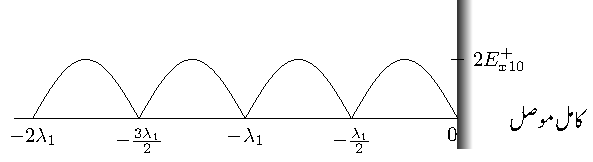
\includegraphics{figWaveStandingWaveVoltageMeasured}
\caption{کامل موصل سے انعکاس، کامل ذو برق میں ساکن موج پیدا کرتا ہے۔}
\label{شکل_موج_ساکن_موج_شکل}
\end{figure}

%==================
\ابتدا{مثال}
کامل موصل سے انعکاس کی صورت میں کامل ذو برق میں ساکن موج کی مساوات حاصل کریں۔

حل:کامل موصل سے انعکاس کی صورت میں \عددیء{\Gamma=-1} حاصل ہوتا ہے  لہٰذا \عددیء{E_{xs1}^-=-E_{x10}^+e^{j\beta_1 z}} ہو گا۔یوں آمدی اور انعکاسی امواج کا مجموعہ
\begin{align*}
E_{xs1}&=E_{x10}^+ e^{-j \beta_1 z} -E_{x10}^+ e^{j \beta_1 z}\\
&=-2 j E_{x10}^+ \sin \beta_1 z
\end{align*}
ہو گا۔اس دوری سمتیہ سے حقیقی ساکن موج کی مساوات حاصل کرنے کی خاطر اسے \عددیء{e^{j\omega t}} سے ضرب دیتے ہوئے
\begin{align*}
E_{xs1} e^{j\omega t}=-2 j E_{x10}^+ \sin \beta_1 z \cos \omega t +2 E_{x10}^+ \sin \beta_1 z \sin \omega t
\end{align*}
 حقیقی جزو
\begin{align*}
E_{x1}=2 E_{x10}^+ \sin \beta_1 z \sin \omega t
\end{align*}
 لیتے ہیں۔یہی ساکن موج کی مساوات ہے۔شکل \حوالہ{شکل_موج_ساکن_موج_شکل} میں آلہ ناپ سے حاصل \عددیء{\abs{E_{x1}}} دکھایا گیا ہے۔
\انتہا{مثال}
%================
اب ایسی صورت پر غور کرتے ہیں جہاں تمام کی تمام موج سرحد سے واپس نہیں لوٹتی بلکہ اس کا کچھ حصہ سرحد پار کرتے ہوئے دوسری جانب چلے جاتی ہے۔پہلے خطے میں اب آمدی موج کے علاوہ ایسی انعکاسی موج پائی جاتی ہے جس کا حیطہ آمدی موج سے کم ہوتا ہے۔اگرچہ اب پہلے خطے میں ساکن موج کے ساتھ ساتھ حرکت  کرتی موج بھی پائی جاتی ہے لیکن اس کے باوجود اس کو ساکن موج ہی پکارا جاتا ہے۔اب کسی بھی نقطے پر میدان ہر وقت صفر نہیں رہتا۔ساکن اور حرکت کرتے حصوں کا اندازہ حیطے کی زیادہ سے زیادہ قیمت اور اس کے کم سے کم قیمت کی شرح سے بیان کی جاتی ہے۔اس شرح کو \اصطلاح{شرح ساکن موج}\فرہنگ{شرح ساکن موج}\حاشیہب{standing wave ratio}\فرہنگ{standing wave ratio} کہا اور \عددیء{s} سے ظاہر کیا جاتا ہے۔ 

فرض کریں کہ پہلا خطہ کامل ذو برق ہے جبکہ دوسرا خطہ کوئی بھی مادہ ہو سکتا ہے۔یوں \عددیء{\alpha_1=0} ہو گا۔اب
\begin{align*}
E_{xs1}^+&=E_{x10}^+ e^{-j\beta_1 z}\\
E_{xs1}^-&=\Gamma E_{x10}^+ e^{j\beta_1 z}
\end{align*}
ہوں گے جہاں
\begin{align*}
\Gamma=\frac{\eta_2-\eta_1}{\eta_2+\eta_1}
\end{align*}
ہے۔چونکہ کامل ذو برق میں \عددیء{\sigma=0} ہوتا ہے لہٰذا \عددیء{\eta_1} مثبت حقیقی عدد ہے جبکہ \عددیء{\eta_2} مخلوط عدد ہو سکتا ہے لہٰذا \عددیء{\Gamma} بھی مخلوط ہو سکتا ہے۔یوں اسے
\begin{align*}
\Gamma=\abs{\Gamma}e^{j \phi}
\end{align*}
بھی لکھا جا سکتا ہے۔یوں
\begin{align*}
E_{xs1}^-&=\abs{\Gamma} E_{x10}^+ e^{j(\beta_1 z+\phi)}
\end{align*}
لکھا جا سکتا ہے جس سے ساکن موج کی مساوات
\begin{align}\label{مساوات_موج_ساکن_مخلوط_موج}
E_{xs1}=\left(e^{-j\beta_1 z}+\abs{\Gamma} e^{j(\beta_1z +\phi)} \right) E_{x10}^+
\end{align}
حاصل ہوتی ہے۔


اب آپ جانتے ہیں کہ کسی بھی مخلوط عدد \عددیء{e^{j\theta}} کو
\begin{align*}
e^{j\theta}=\cos \theta+j \sin \theta
\end{align*}
لکھا جا سکتا ہے۔چونکہ \عددیء{\cos^2 \theta+\sin^2 \theta=1} ہوتا ہے لہٰذا اس کی حتمی قیمت ایک \عددیء{(1)} ہی رہتی ہے۔اس عدد کی زیادہ سے زیادہ قیمت
 \عددیء{\theta=0} کی صورت میں \عددیء{+1} حاصل ہوتی ہے۔یہی قیمت \عددیء{{\theta=\mp 2\pi}} یا \عددیء{{\theta=\mp 4\pi}} کی صورت میں بھی حاصل ہوتی ہے۔اسی طرح اس کی کم سے کم قیمت \عددیء{{\theta=\mp\pi,\mp 3\pi,\mp5\pi\cdots}} پر \عددیء{-1} حاصل ہوتی ہے۔اس طرح مساوات \حوالہ{مساوات_موج_ساکن_مخلوط_موج} کو
\begin{align*}
E_{xs1}=\left(1+\abs{\Gamma} e^{j(2\beta_1z +\phi)} \right) e^{-j \beta_1 z} E_{x10}^+
\end{align*}
لکھتے ہوئے  اگر  \عددیء{2 \beta_1 z+\phi} کو \عددیء{\theta} تصور کیا جائے تو  \عددیء{e^{j(2\beta_1 z +\phi)}} کی زیادہ سے زیادہ قیمت یعنی \عددیء{+1}
\begin{align*}
2\beta_1 z +\phi=0, 2\pi,-2\pi,4\pi,-4\pi,\cdots
\end{align*}
پر حاصل ہو گی۔اس مساوات کو
\begin{align}\label{مساوات_موج_مقام_بلنتر_دباو}
-\beta_1 z_{\text{بلندتر}} =\frac{\phi}{2}+ n \pi \quad (n=0,\mp1,\mp 2, \cdots)
\end{align}
لکھا جا سکتا ہے۔ ایسی صورت میں
\begin{align}
\abs{E_{xs1}}_{\text{\RL{بلندتر}}}=\left(1+\abs{\Gamma} \right)E_{x10}^+
\end{align}
ہو گا۔ 

\عددی{\eta_2 \gg \eta_1} کی صورت میں \عددی{\Gamma=1\phase{0^{\circ}}} حاصل ہوتا ہے۔یوں سرحد پر ساکن موج کی چوٹی پائی جائے گی۔اگلی چوٹی سرحد سے \عددی{\tfrac{\lambda}{2}} فاصلے پر ہو گی۔\عددی{\eta_2} اور \عددی{\eta_1} کے کسی بھی اور قیمت کی صورت میں سرحد اور پہلی چوٹی کے درمیان فاصلہ \عددی{\tfrac{\lambda}{2}} سے کم ہو گا۔

اسی طرح \عددیء{e^{j(2\beta_1 z +\phi)}} کی کم سے کم قیمت یعنی \عددیء{-1}
\begin{align*}
2\beta_1 z +\phi= \pi, -\pi, 3\pi, -3\pi,\cdots
\end{align*}
پر حاصل ہو گی۔ اس مساوات کو
\begin{align}\label{مساوات_موج_مقام_بلنتر_دباو_ب}
-\beta_1 z_{\text{کمتر}} =\frac{\phi}{2}+n\pi+\frac{\pi}{2} \quad (n=0,\mp 1,\mp 2,\cdots)
\end{align}
لکھا جا سکتا ہے اور ایسی صورت میں
\begin{align}\label{مساوات_موج_کمتر_قیمت}
\abs{E_{xs1}}_{\text{\RL{کمتر}}}=\left(1-\abs{\Gamma} \right)E_{x10}^+
\end{align}
ہو گا۔

\عددی{\eta_2 \ll \eta_1} کی صورت میں سرحد پر ساکن موج کی کمتر قیمت پائی جائے گی۔اگلی کمتر قیمت سرحد سے \عددی{\tfrac{\lambda}{2}} فاصلے پر ہو گی۔\عددی{\eta_2} اور \عددی{\eta_1} کے کسی بھی اور قیمت کی صورت میں سرحد اور پہلی کمتر نقطے کے درمیان فاصلہ \عددی{\tfrac{\lambda}{2}} سے کم ہو گا۔

مساوات \حوالہ{مساوات_موج_مقام_بلنتر_دباو} سے \عددی{z_{\text{بلندتر}}} اور مساوات \حوالہ{مساوات_موج_مقام_بلنتر_دباو_ب} سے \عددی{z_{\text{کمتر}}} حاصل کرتے ہوئے دھیان رہے کہ صرف ان قیمتوں کو درست تصور کیا جائے جو شکل \حوالہ{شکل_موج_غیر_کامل_ذوبرق_ساکن_موج} میں ٹھیک طرف پائے جاتے ہوں یعنی \عددی{z_{\text{بلندتر}}} اور \عددی{z_{\text{کمتر}}}  کی قیمت منفی ہونی چاہیے۔

موج کی کم تر قیمت ہر آدھے طول موج پر پائی جاتی ہے۔موج کی بلند تر قیمت دو کم تر قیمتوں کے مقام کے عین وسط میں پائی جاتی ہیں۔کامل موصل کی صورت میں پہلا کمتر میدان \عددیء{-\beta_1 z =0} یعنی سرحد پر پایا جائے گا۔اگر \عددیء{\eta_2<\eta_1} ہو اور دونوں قدرتی رکاوٹوں کی قیمتیں حقیقی اعداد ہوں تب \عددیء{\phi=\pi} ہو گا اور ایسی صورت میں سرحد یعنی \عددیء{-\beta_1 z =0} پر برقی دباو کی کمتر قیمتیں پائی جائے گی۔اس کے برعکس اگر \عددیء{\eta_2>\eta_1} ہو اور دونوں رکاوٹ حقیقی ہوں تب سرحد پر برقی میدان کی قیمت بلند تر ہو گی۔  

ان معلومات کو زیر استعمال لانے کی غرض سے \عددیء{\SI{10}{\volt \per \meter}} اور \عددیء{\SI{1}{\giga\hertz}} تعدد کے موج پر غور کرتے ہیں جو خطہ اول میں سرحد کی طرف عمودی آمد ہے۔پہلے خطے کے مستقل \عددیء{\epsilon_{R1}=3}، \عددیء{\mu_{R1}=1} اور \عددیء{\sigma_{1}=0} جبکہ دوسرے خطے کے مستقل
 \عددیء{\epsilon_{R1}=6}، \عددیء{\mu_{R1}=1} اور \عددیء{\sigma_{1}=0} ہیں۔

یوں 
\begin{align*}
\omega=2 \pi 10^9 \, \si{\radian \per \second}, \quad \beta_1=\SI{36.28}{\radian \per \meter}, \quad \beta_2=\SI{51.3}{\radian \per \meter}
\end{align*}
حاصل ہوتے ہیں۔اگرچہ خالی خلاء میں اس موج کی طول \عددیء{\SI{30}{\centi\meter}} ہو گی، یہاں \عددیء{\lambda_1=\SI{17.32}{\centi\meter}}  اور \عددیء{\lambda_2=\SI{12.25}{\centi\meter}} ہیں۔قدرتی رکاوٹ \عددیء{\eta_1=\SI{217.66}{\ohm}} اور \عددیء{\eta_2=\SI{153.91}{\ohm}} ہیں جن سے شرح انعکاس \عددیء{\Gamma=-0.17} حاصل ہوتا ہے۔ چونکہ دونوں رکاوٹ حقیقی اعداد ہیں اور \عددیء{\eta_2<\eta_1} ہے لہٰذا سرحد پر کمتر برقی میدان پایا جائے گا۔پہلے خطے، یعنی  \عددیء{z<0}،  میں سرحد سے دور ہر \عددیء{\SI{8.66}{\centi\meter}} فاصلے پر برقی میدان کی کمتر قیمت پائی جائے گی۔مساوات \حوالہ{مساوات_موج_کمتر_قیمت} سے ساکن موج کی کمتر قیمت \عددیء{\abs{Exs1}_{\text{کمتر}}=\SI{8.3}{\volt\per\meter}} حاصل ہوتی ہے۔چونکہ پہلا خطہ کامل ذو برق ہے لہٰذا اس میں طاقت کا ضیاع نہیں ہوتا اور یوں اس خطے میں تمام کمتر قیمتیں برابر ہوں گی۔

میدان کی بلند تر قیمت \عددیء{\SI{11.7}{\volt\per\meter}} پہلے خطے میں سرحد سے  \عددی{4.33}، \عددی{12.99}، \عددی{21.65} ،\عددی{\cdots} سنٹی میٹر کے فاصلوں پر پائی جائیں گی۔

چونکہ دوسرے خطے میں انعکاسی موج نہیں پائی جاتی لہٰذا اس میں ساکن موج بھی نہیں پائی جائے گی۔

ساکن موج کی زیادہ سے زیادہ اور کم سے کم قیمتوں کی شرح کو \اصطلاح{شرح ساکن موج}\فرہنگ{شرح ساکن موج}\حاشیہب{standing wave ration}\فرہنگ{standing wave ration} کہا اور \عددیء{s} سے ظاہر کیا جاتا ہے۔
\begin{align}
s=\frac{\phantom{\,}\abs{E_{xs1}}_{\text{\RL{بلندتر}}}}{\abs{E_{xs1}}_{\text{\RL{کمتر}}}}=\frac{1+\abs{\Gamma}}{1-\abs{\Gamma}}
\end{align}
چونکہ \عددیء{\abs{\Gamma} \le 1 } رہتا ہے لہٰذا شرح ساکن موج ہر صورت مثبت اور اکائی کے برابر یا اس سے زیادہ قیمت کا ہو گا یعنی
\begin{align}
s \ge 1 
\end{align}
مندرجہ بالا مثال میں \عددیء{s=\tfrac{1+0.17}{1-0.17}=1.409} ہے۔

اگر \عددیء{\abs{\Gamma}=1} ہو تب انعکاسی اور آمدی امواج برابر ہوں گے لہٰذا تمام کی تمام آمدی توانائی سرحد سے واپس لوٹتی ہے اور ایسی صورت میں \عددیء{s} لامحدود ہو گا۔پہلے خطے میں ہر \عددیء{\tfrac{\lambda_1}{2}} فاصلے پر ایسی سطح  پائی جائے گی جس پر برقی میدان ہر وقت صفر رہتا ہے۔ان سطحوں کے درمیان ایسی سطحیں ہوں گی جہاں آمدی موج کے دگنے حیطے کا برقی میدان ہو گا۔

اگر \عددیء{\eta_2=\eta_1} ہو تب \عددیء{\Gamma=0} ہو گا۔ایسی صورت میں توانائی سرحد سے واپس نہیں لوٹتی، \عددیء{s=1} ہوتا ہے اور برقی میدان کی بلند تر اور کم تر قیمتیں برابر ہوتی ہیں۔

آدھی طاقت کے انعکاس کی صورت میں \عددیء{\abs{\Gamma}^2=0.5} یعنی \عددیء{\abs{\Gamma}=0.707} اور \عددیء{s=5.83} ہو گا۔ 

چونکہ برقی اور مقناطیسی میدان کے راست تناسب اشارات باآسانی حاصل کئے جا سکتے ہیں اور \عددیء{s} کی قیمت حاصل کرنے کے لئے راست تناسب اشارات ہی درکار ہیں لہٰذا شرح ساکن موج کو تجرباتی طور حاصل کیا جا سکتا ہے۔یہی اس کی اہمیت کا راز ہے۔یاد رہے کہ \عددیء{s} حاصل کرنے کے لئے میدان کی اصل قیمت درکار نہیں ہوتی۔صرف اتنا ضروری ہوتا ہے کہ تمام اشارات اصل میدان کے تناسب سے ہوں۔

\begin{figure}
\centering
\includegraphics{figWaveOctaveStandingWaveLossyMedium}
\caption{غیر کامل ذو برق میں ساکن موج کی بلند تر اور کم تر قیمتوں میں فرق سرحد سے دور کم ہوتا ہے۔}
\label{شکل_موج_غیر_کامل_ذوبرق_ساکن_موج}
\end{figure}

آئیں اب پہلے خطے کو غیر کامل ذو برق تصور کریں جس کا \عددیء{\alpha} صفر کے برابر نہیں ہو گا۔اب بائیں سے آتی آمدی موج مثبت \عددیء{z} جانب چلتے ہوئے گھٹے گی۔انعکاسی موج منفی \عددیء{z} جانب چلتے ہوئے گھٹتے جائے گی حتٰی کہ آخر کار اس کی قیمت قابل نظر انداز ہو گی۔یوں اگرچہ سرحد کے قریب بلند تر اور کم تر میدان میں فرق  واضح ہو سکتا ہے لیکن سرحد سے دور ان میں فرق نہیں رہ پاتا۔ پہلے خطے کا حرکی مستقل \عددیء{\gamma_1=1+j5\pi} اور دوسرا خطہ کامل موصل ہونے کی صورت میں ایسی ہی ایک ساکن موج شکل \حوالہ{شکل_موج_غیر_کامل_ذوبرق_ساکن_موج} میں دکھائی گئی ہے جہاں موصل \عددیء{z=0} کے دائیں ہاتھ پر ہے۔اس شکل میں عین سرحد پر آمدی
 موج کی قیمت \عددیء{E_{x10}^+=\SI{1}{\volt\per\meter}} ہے۔چونکہ ذو برق کا سرحد موصل کے ساتھ ہے اور موصل میں برقی میدان صفر ہوتا ہے لہٰذا شکل میں سرحد پر برقی میدان صفر ہی ہے۔سرحد سے \عددیء{\tfrac{2\pi}{\beta_1}=\SI{0.2}{\meter}} فاصلے پر دوبارہ کم تر میدان پایا جاتا ہے۔اسی طرح  پہلی چوٹی سرحد پر آمدی میدان کے تقریباً  دگنی ہے۔آپ دیکھ سکتے ہیں کہ کوئی بھی دو چوٹیاں یا دو نشیب برابر نہیں ہیں۔یہاں شرح ساکن موج کی قیمت اس صورت مطلب رکھتی ہے جب اسے ناپنے کا مقام یعنی \عددیء{z} بھی ساتھ بتلایا جائے۔ایسی صورت میں انعکاسی شرح اور تضعیفی مستقل زیادہ کار آمد معلومات ہیں۔

اگرچہ مندرجہ بالا مثال زیادہ انتہا درجے کا تھا لیکن یہ بھی نہیں بھولنا چاہئے کہ حقیقت میں کامل ترسیلی تار بھی نہیں پائے جاتے۔حقیقت میں شرح ساکن موج ہر صورت سرحد سے فاصلے پر منحصر ہو گی اور اس کا استعمال اسی وقت ممکن ہو گا جب ہماری دلچسپی کے خطے میں اس کی قیمت زیادہ تبدیل نہ ہو۔   

آئیں دوبارہ پہلا خطہ کامل ذو برق لیتے ہوئے برقی اور مقناطیسی میدان کی شرح حاصل کریں۔لامحدود حجم میں آزاد موج کی صورت میں یہ شرح \عددیء{\eta_1} تھی۔انعکاسی موج کی موجودگی میں برقی اور مقناطیسی میدان صفر بھی ممکن ہیں لہٰذا ان کی شرح صفر سے لامحدود قیمت کی ہو سکتی ہے۔سرحد سے \عددیء{z=-l} فاصلے پر میدان
 \begin{align*}
E_{xs1}&=\left(e^{j \beta_1 l}+ \Gamma e^{-j \beta_1 l} \right)E_{x10}^+ \\
H_{ys1}&=\left(e^{j \beta_1 l}- \Gamma e^{-j \beta_1 l} \right) \frac{E_{x10}^+}{\eta_1}
\end{align*}
ہیں۔ان کی شرح کو \اصطلاح{داخلی قدرتی رکاوٹ}\فرہنگ{داخلی قدرتی رکاوٹ}\فرہنگ{قدرتی رکاوٹ!داخلی}\فرہنگ{رکاوٹ!داخلی قدرتی}\حاشیہب{intrinsic input impedance}\فرہنگ{intrinsic input impedance} کہتے اور \عددیء{\eta_{\text{داخلی}}} سے ظاہر کیا جاتا ہے۔
\begin{align*}
\eta_{\text{داخلی}}=\left. \frac{E_{xs1}}{H_{ys1}} \right|_{z=-l}=\eta_1 \frac{e^{j \beta_1 l}+ \Gamma e^{-j \beta_1 l}}{e^{j \beta_1 l}- \Gamma e^{-j \beta_1 l}}
\end{align*}
اس میں \عددیء{\Gamma=\tfrac{\eta_2-\eta_1}{\eta_2+\eta_1}} پر کرتے ہوئے اور  \اصطلاح{یولر مماثل}\فرہنگ{یولر مماثل}\حاشیہد{$e^{j \alpha}=\cos \alpha+j \sin \alpha$} استعمال کرتے ہوئے
\begin{align*}
\eta_{\text{داخلی}}=\eta_1 \frac{(\eta_2+\eta_1)(\cos \beta_1 l +j \sin \beta_1 l)+(\eta_2-\eta_1)(\cos \beta_1 l -j \sin \beta_1 l)}{(\eta_2+\eta_1)(\cos \beta_1 l +j \sin \beta_1 l)-(\eta_2-\eta_1)(\cos \beta_1 l -j \sin \beta_1 l)}
\end{align*}
حاصل ہوتا ہے  جسے باآسانی یوں
\begin{align}\label{مساوات+موج_ترسیلی_نظام_داخلی_قدرتی_رکاوٹ_تعریف}
\eta_{\text{داخلی}}=\eta_1 \frac{\eta_2 +j \eta_1 \tan \beta_1 l}{\eta_1+j \eta_2 \tan \beta_1 l}
\end{align}
لکھا جا سکتا ہے۔

جب \عددیء{\eta_2} اور \عددیء{\eta_1} برابر ہوں تب داخلی قدرتی رکاوٹ \عددیء{\eta_{\text{داخلی}}} پہلے خطے کی قدرتی رکاوٹ \عددیء{\eta_1} کے برابر ہوتی ہے۔ایسی صورت میں انعکاس پیدا نہیں ہوتی اور  ترسیلی نظام \اصطلاح{ہم رکاوٹی}\فرہنگ{ہم رکاوٹی}\حاشیہب{matched}\فرہنگ{matched} کہلاتا ہے۔ہم رکاوٹی نظام میں انعکاس کے غیر موجودگی کی بنا توانائی ایک ہی سمت میں منتقل ہوتی ہے۔اگر دوسرا خطہ کامل موصل ہو تب \عددیء{{\eta_2=0}} ہو گا۔ایسی صورت میں
\begin{align}
\eta_{\text{داخلی}}=j \eta_1 \tan \beta_1 l \quad (\eta_2=0)
\end{align}
ہو گا لہٰذا ان مقامات پر جہاں \عددیء{E_{xs1}=0} ہو، یعنی جب \عددیء{\beta_1 l = n \pi} ہو، داخلی قدرتی رکاوٹ صفر کے برابر ہو گی جبکہ ان مقامات پر جہاں \عددیء{H_{ys1}=0} ہو وہاں داخلی قدرتی رکاوٹ لامحدود ہو گی۔

مساوات \حوالہ{مساوات+موج_ترسیلی_نظام_داخلی_قدرتی_رکاوٹ_تعریف} ترسیلی نظام پر غور کرنے کے لئے انتہائی اہمیت کا حامل ہے۔

%=========================================
\حصہ{دو سرحدی انعکاس}
اب تک ہم دو ایسے خطوں کے سرحد پر موج کی انعکاس پر غور کرتے رہے ہیں جن میں دونوں خطے نیم لامحدود جسامت کے تھے۔\اصطلاح{نیم لامحدود خطے}\فرہنگ{نیم لامحدود خطہ}\حاشیہب{semi-infinity region}\فرہنگ{semi-infinite region} سے مراد ایسا خطہ ہے جس کی ایک سرحد محدود فاصلے پر اور دوسری سرحد لامحدود فاصلے پر ہو۔ایسی صورت میں سرحد پار کرنے کے بعد ترسیلی موج دوسرے خطے میں مسلسل آگے ہی بڑھتے ہے اور ایسا کوئی امکان نہیں پایا جاتا کہ یہ لامحدود فاصلے پر موجود  سرحد سے انعکاس پذیر ہو کر واپس پہلی سرحد تک آن پہنچے۔اس حصے میں ہم محدود جسامت کے خطے میں ترسیلی موج پر غور کرتے ہیں جہاں دوسرے خطے کی محدود جسامت کی بنا پر ترسیلی موج کا کچھ حصہ واپس پہلی سرحد پر پہنچ سکتا ہے۔

شکل \حوالہ{شکل_مستوی_دو_سرحد_مسئلہ} میں دو سرحدی مسئلہ دکھایا گیا ہے جہاں پہلے نیم لامحدود خطے کی قدرتی رکاوٹ \عددی{\eta_1}، دوسرے محدود موٹائی کے خطے کی قدرتی رکاوٹ \عددی{\eta_2} اور تیسرے نیم لامحدود خطے کی قدرتی رکاوٹ \عددی{\eta_3} ہے۔محدود خطے کی موٹائی \عددی{l} ہے۔یہاں پہلا سرحد خطہ-1 اور خطہ-2 کے درمیان \عددی{z=-l} پر جبکہ دوسرا سرحد خطہ-2 اور خطہ-3 کے درمیان \عددی{z=0} پر پایا جاتا ہے۔پہلے خطے میں موج دائیں جانب (یعنی بڑھتے \عددی{z} جانب) حرکت کرتے ہوئے پہلی سرحد پر عمودی آن پہنچتی ہے جس کے بعد یہ مسلسل چلی آتی ہے۔

پہلی سرحد پر آمدی موج کا کچھ حصہ انعکاس پذیر ہو کر واپس پہلے خطے میں بائیں جانب لوٹتا ہے جبکہ اس کا بقایا حصہ دوسرے خطے میں داخل ہو کر دائیں جانب حرکت کرتے ہوئے دوسری سرحد پر پہنچتا ہے۔اس موج کا کچھ حصہ دوسری سرحد سے بھی گزر پاتا ہے جبکہ اس کا بقایا حصہ دوسرے سرحد سے انعکاس پذیر ہو کر واپس پہلی سرحد جانب چل پڑتا ہے جہاں انعکاس اور ترسیل کا عمل ایک مرتبہ دوبارہ دہرایا جاتا ہے۔یوں دوسرے سرحد سے واپس لوٹتی موج کا کچھ حصہ پہلی سرحد سے گزر کر پہلے خطے میں داخل ہو کر تازہ انعکاسی موج کے ساتھ مل کر بائیں چلے جاتا ہے جبکہ اس کا بقایا حصہ پہلی سرحد سے انعکاس پذیر ہو کر اسی سرحد سے تازہ ترسیلی موج کے ساتھ مل کر  دوسری سرحد کے جانب چل پڑتا ہے۔یہی عمل بار بار دہرایا جاتا ہے۔

یوں ہر لمحہ پہلے خطے سے تازہ ترسیلی موج دوسرے خطے میں داخل ہو کر، اس خطے میں پہلے سے موجود، متعدد مرتبہ انعکاس پذیر اجزاء کے ساتھ مل کر دوسری سرحد کی جانب ایک نئی کارواں روانہ کرتی ہے۔اسی طرح دوسرے خطے میں بار بار انعکاس پذیر اور پہلی سرحد سے دو مرتبہ ترسیل کے بعد متعدد حصے مل کر پہلے خطے میں مجموعی انعکاسی موج کو جنم دیتے ہیں۔  
ہم اسی طرح تمام امواج کو مد نظر رکھتے ہوئے مسئلے کو حل کر سکتے ہیں۔صفحہ \حوالہصفحہ{حصہ_ترسیلی_عارضی_حال} پر حصہ \حوالہ{حصہ_ترسیلی_عارضی_حال} میں ایسا ہی کرتے ہوئے عارضی حالت دریافت کی گئی ہے۔

\begin{figure}
\centering
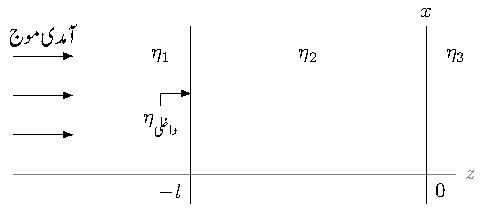
\includegraphics{figWaveTwoBoundaryReflection}
\caption{دو سرحدی  مسئلے میں دوسرے اور تیسرے خطے کے قدرتی رکاوٹ اور دوسرے خطے کی موٹائی کے اثرات پہلی سرحد پر داخلی قدرتی رکاوٹ کی صورت میں نمودار ہوتے ہیں۔}
\label{شکل_مستوی_دو_سرحد_مسئلہ}
\end{figure}

اگر آمدی موج برقرار آتی رہے  تب تینوں خطوں میں جلد برقرار صورت حال پیدا ہو جاتی ہے جہاں پہلے خطے میں آمدی موج کی نسبت سے کوئی خاص مقدار کی موج بطور انعکاسی موج پائی جاتی ہے۔اس انعکاسی موج کا مخصوص حیطہ اور دوری زاویہ پایا جاتا ہے۔اسی طرح دونوں سرحد سے گزرتے ہوئے ،تیسرے خطے میں بھی آمدی موج کی نسبت سے کوئی خاص مقدار کی موج بطور ترسیلی موج پائی جاتی ہے جس کا مخصوص حیطہ اور دوری زاویہ پایا جاتا ہے۔دوسرے خطے میں پہلی سرحد سے تازہ ترسیلی اور دوسرے خطے میں واپس انعکاسی امواج مل کر مخصوص حیطے اور دوری زاویے کی موج کو جنم دیتے ہیں جو پہلی سرحد سے دوسری سرحد کی جانب گامزن پائی جاتی ہے۔اسی طرح دوسرے خطے میں دوسری سرحد سے تمام انعکاس پذیر امواج کا مجموعہ بطور انفرادی موج ابھرتا ہے جس کا مخصوص حیطہ اور دوری زاویہ ہوتا ہے۔ یوں برقرار صورت حال حاصل کرنے کے بعد کل پانچ عدد امواج پائے جاتے ہیں یعنی پہلے خطے میں آمدی اور انعکاسی موج، تیسرے خطے میں ترسیلی موج اور دوسرے خطے میں دائیں حرکت کرتی موج اور بائیں حرکت کرتی موج۔آئیں ان پانچ عدد امواج کی مدد سے مسئلے کو حل کریں۔

ہم تصور کرتے ہیں کہ تینوں خطے بے ضیاع، غیر مقناطیسی ہیں اور برقی میدان \عددی{x} سمت میں ہے۔ یوں دوسرے خطے میں دائیں اور بائیں جانب حرکت کرتے ہوئے امواج مل کر برقی میدان 
\begin{align}
E_{xs2}=E_{x20}^+ e^{-j\beta_2 z}+E_{x20}^- e^{j \beta_2 z}
\end{align}
پیدا کرتے ہیں جہاں \عددی{\beta_2=\tfrac{\omega \sqrt{\epsilon_{R2}}}{c}} ہے جبکہ \عددی{E_{x20}^+} اور \عددی{E_{x20}^-} مخلوط مقدار ہیں۔مقناطیسی میدان \عددی{y} سمت میں ہو گا۔یوں مقناطیسی میدان
\begin{align}
H_{ys2}=H_{y20}^+ e^{-j\beta_2 z}+H_{y20}^- e^{j \beta_2 z}
\end{align}
لکھا جائے گا۔دوسرے خطے میں بائیں اور دائیں حرکت کرتے برقی امواج دوسری سرحد کے انعکاسی مستقل \عددی{\Gamma_{23}} سے وابستہ ہیں جہاں
\begin{align}\label{مساوات_مستوی_دو_سرحد_انعکاسی_مستقل_دو}
\Gamma_{23}=\frac{\eta_3-\eta_2}{\eta_3+\eta_2}
\end{align}
کے برابر ہے۔یوں
\begin{align}\label{مساوات_مستوی_دو_سرحد_برقی_دو}
E_{x20}^-=\Gamma_{23} E_{x20}^+
\end{align}
لکھا جا سکتا ہے۔مقناطیسی اجزاء کو یوں 
\begin{align}\label{مساوات_مستوی_دو_سرحد_مقناطیسی_دو}
H_{y20}^+&=\frac{E_{x20}^+}{\eta_2}\\
H_{y20}^-&=-\frac{E_{x20}^-}{\eta_2}=-\frac{\Gamma_{23} E_{20}^+}{\eta_2}
\end{align}
لکھا جا سکتا ہے۔

برقی میدان تقسیم مقناطیسی  میدان کو \اصطلاح{رکاوٹ موج}\فرہنگ{رکاوٹ موج}\فرہنگ{رکاوٹ موج}\حاشیہب{wave impedance}\فرہنگ{impedance!wave} \عددی{\eta_m} کہا جاتا ہے۔ 
\begin{align}
\eta_m(z)=\frac{E_{xs2}}{H_{ys2}}=\frac{E_{x20}^+ e^{-j\beta_2 z}+E_{x20}^- e^{j \beta_2 z}}{H_{y20}^+ e^{-j\beta_2 z}+H_{y20}^- e^{j \beta_2 z}}
\end{align}
مساوات \حوالہ{مساوات_مستوی_دو_سرحد_برقی_دو} اور مساوات \حوالہ{مساوات_مستوی_دو_سرحد_مقناطیسی_دو} استعمال کرتے ہوئے اسے
\begin{align}
\eta_m(z)=\eta_2 \left[\frac{e^{-j \beta_2 z}+\Gamma_{23} e^{j \beta_2 z}}{e^{-j \beta_2 z}-\Gamma_{23} e^{j \beta_2 z}} \right]
\end{align}
لکھا جا سکتا ہے۔مساوات \حوالہ{مساوات_مستوی_دو_سرحد_انعکاسی_مستقل_دو} اور یولر مماثل\حاشیہب{Euler's identity} کے استعمال سے اسے یوں لکھا جا سکتا ہے۔
\begin{align}\label{مساوات_مستوی_موج_کی_رکاوٹ}
\eta_m(z)=\eta_2 \frac{\eta_3 \cos \beta_2 z - j \eta_2 \sin \beta_2 z}{\eta_2 \cos \beta_2 z - j \eta_3 \sin \beta_2 z}
\end{align}

مندرجہ بالا مساوات دوسرے خطے میں موج کی رکاوٹ دیتی ہے۔اسے استعمال کرتے ہوئے پہلی سرحد پر کل انعکاسی موج حاصل کرتے ہیں۔چونکہ سرحد پر متوازی برقی میدان \عددی{\kvec{E}} اور متوازی مقناطیسی میدان \عددی{\kvec{H}} ہموار ہیں لہٰذا
\begin{align}
E_{xs1}^++E_{xs1}^-&=E_{xs2} \quad \quad (z=-l)\\
H_{ys1}^++H_{ys1}^-&=H_{ys2} \quad \quad (z=-l)
\end{align}
لکھا جا سکتا ہے۔ان مساوات کو
\begin{align}
E_{x10}^+ + E_{x10}^- &=E_{xs2} \quad \quad (z=-l)\\
\frac{E_{x10}}{\eta_1}-\frac{E_{x10}^-}{\eta_1}&=\frac{E_{xs2}}{\eta_m(-l)} \quad \quad (z=-l)
\end{align}
لکھا\حاشیہد{ایسا اس لمحے لکھا جا سکتا ہے جب آمدی موج کا حیطہ عین پہلی سرحد پر پایا جاتا ہو۔} جا سکتا ہے جہاں پہلے خطے میں آمدی موج کا حیطہ \عددی{E_{x10}^+} اور مجموعی انعکاسی موج کو حیطہ \عددی{E_{x10}^-} ہے۔ان دونوں مساوات میں دائیں ہاتھ \عددی{E_{xs2}} کو جوں کا توں لکھا گیا ہے جبکہ \عددی{z=-l} پر موج کے رکاوٹ کی قیمت  استعمال کی گئی ہے۔\عددی{z=-l}  پر موج کے رکاوٹ کو پہلی سرحد پر داخلی قدرتی رکاوٹ\فرہنگ{داخلی قدرتی رکاوٹ}\فرہنگ{قدرتی رکاوٹ!داخلی} \عددی{\eta_{\text{داخلی}}} لکھتے ہوئے مندرجہ بالا دو مساوات کو حل کرتے ہوئے \عددی{E_{xs2}} سے چھٹکارا حاصل کرتے ہیں۔یوں
\begin{align}\label{مساوات_مستوی_شرح_انعکاس_دو_سرحدی}
\frac{E_{x10}^-}{E_{x10}^+}=\Gamma=\frac{\eta_{\text{داخلی}}-\eta_1}{\eta_{\text{داخلی}}+\eta_1}
\end{align}
حاصل ہوتا ہے۔ پہلی سرحد پر داخلی قدرتی رکاوٹ مساوات \حوالہ{مساوات_مستوی_موج_کی_رکاوٹ} میں \عددی{z=-l} پر کرنے سے
\begin{align}\label{مساوات_مستوی_داخلی_رکاوٹ_دو_سرحدی}
\eta_{\text{داخلی}}= \eta_2 \frac{\eta_3 \cos \beta_2 l +j \eta_2 \sin \beta_2 l}{\eta_2 \cos \beta_2 l +j \eta_3\sin \beta_2 l}
\end{align}
یا
\begin{align}\label{مساوات_مستوی_داخلی_رکاوٹ_دو_سرحدی_ب}
\eta_{\text{داخلی}}= \eta_2 \frac{\eta_3  +j \eta_2 \tan \beta_2 l}{\eta_2  +j \eta_3\tan \beta_2 l}
\end{align}
حاصل ہوتا ہے۔  یہاں رک کر ایک مرتبہ مساوات \حوالہ{مساوات_مستوی_داخلی_رکاوٹ_دو_سرحدی_ب} کا مساوات \حوالہ{مساوات+موج_ترسیلی_نظام_داخلی_قدرتی_رکاوٹ_تعریف} کے ساتھ موازنہ کریں۔

مساوات \حوالہ{مساوات_مستوی_شرح_انعکاس_دو_سرحدی} اور مساوات \حوالہ{مساوات_مستوی_داخلی_رکاوٹ_دو_سرحدی} عمومی مساوات ہیں جن سے  بے ضیاع، دو متوازی سرحد سے  مجموعی انعکاسی موج کا حیطہ اور دوری زاویہ حاصل کیے جا سکتے ہیں۔پہلے خطے میں آمدی طاقت کا  \عددی{\Gamma^2} حصہ مجموعی انعکاسی طاقت ہو گا۔آمدی طاقت کا \عددی{1-\Gamma^2} حصہ دوسرے خطے سے ہوتا ہوا تیسرے خطے میں ترسیل ہو گا۔دوسرے خطے میں بائیں جانب سے جتنی طاقت داخل ہوتی ہے، اس سے اتنی ہی طاقت دائیں جانب خارج ہوتی ہے۔

مساوات \حوالہ{مساوات_مستوی_شرح_انعکاس_دو_سرحدی} میں \عددی{\eta_{\text{داخلی}}=\eta_1} کی صورت میں \عددی{\Gamma=0} حاصل  ہوتا ہے جس سے انعکاسی طاقت صفر کے برابر ہو جاتی ہے۔ایسی صورت میں تمام کی تمام آمدی طاقت تیسرے خطے میں داخل ہو پاتی ہے۔ایسا معلوم ہوتا ہے جیسے دوسرا خطہ موجود ہی نہیں ہے۔ایسی صورت میں ہم کہتے ہیں کہ داخلی قدرتی رکاوٹ اور پہلا خطہ \اصطلاح{ہم رکاوٹ}\فرہنگ{ہم رکاوٹ}\حاشیہب{matched}\فرہنگ{matched} ہیں۔ہم رکاوٹ صورت کئی طریقوں سے حاصل کرنا ممکن ہے۔یہاں \عددی{\eta_3=\eta_1} کی صورت میں ہم رکاوٹی حالت حاصل کرتے ہیں۔حصہ \حوالہ{حصہ_مستوی_دو_سرحدی_ہم_رکاوٹ_عمومی_حل} میں \عددی{\eta_3\ne\eta_1} کی صورت میں ہم رکاوٹی حالت اختیار کرنا دکھایا جائے گا۔

اگر پہلے اور تیسرے خطے کے قدرتی رکاوٹ برابر ہوں، یعنی \عددی{\eta_1=\eta_3} ہوں، تب \عددی{\beta_2 l =m \pi} جہاں \عددی{m=1,2,3,\cdots} ہو کی صورت میں مساوات \حوالہ{مساوات_مستوی_داخلی_رکاوٹ_دو_سرحدی} سے  \عددی{\eta_{\text{داخلی}}=\eta_1} حاصل ہوتا ہے۔ چونکہ \عددی{\beta_2=\tfrac{2\pi}{\lambda_2}} کے برابر ہے جہاں \عددی{\lambda_2} دوسرے خطے میں طول موج ہے لہٰذا
\begin{align*}
\frac{2 \pi}{\lambda_2}=m \pi
\end{align*}
یا
\begin{align}\label{مساوات_مستوی_دو_سرحدی_ہم_رکاوٹ_شرط}
l=\frac{m \lambda_2}{2}
\end{align}
درکار شرط ہے۔مساوات \حوالہ{مساوات_مستوی_دو_سرحدی_ہم_رکاوٹ_شرط} کے مطابق دوسرے خطے کی موٹائی دوسری خطے میں طول موج کی آدھی یا اس کے \عددی{m} گنا درکار ہے۔ایسی صورت میں \عددی{{\eta_{\text{داخلی}}=\eta_1}} حاصل ہوتا ہے۔اس ترکیب سے ہم رکاوٹ صورت حال حاصل کرنے کو \اصطلاح{نصف طول موج}\فرہنگ{نصف طول موج}\حاشیہب{half-wave matching}\فرہنگ{half-wave matching} کی ترکیب کہا جاتا ہے۔

نصف طول موج ترکیب سے تمام آمدی طاقت تیسرے خطے میں منتقل کی جا سکتی ہے۔آمدی موج کی تعدد یعنی اس کی طول موج تبدیل کرنے سے ہم رکاوٹی شرط پوری نہیں ہو پاتی لہٰذا ایسی صورت میں مساوات \حوالہ{مساوات_مستوی_داخلی_رکاوٹ_دو_سرحدی} سے حاصل \عددی{\eta_{\text{داخلی}}} کی قیمت \عددی{\eta_1} سے قدر مختلف ہو گی جس سے \عددی{\Gamma} صفر نہیں رہ پاتا۔طول موج جتنی زیادہ تبدیل کی جائے \عددی{\Gamma} کی قیمت اتنی زیادہ حاصل ہوتی ہے۔ایسی صورت میں دو سرحدی جوڑ بطور \اصطلاح{پٹی گزار فلٹر}\فرہنگ{پٹی گزار فلٹر}\حاشیہب{band pass filter}\فرہنگ{band pass filter} کردار ادا کرتا ہے۔

آئیں دو سرحدی مسئلے کے حقیقی مثال پر غور کریں۔
%========================================

\begin{figure}
\centering
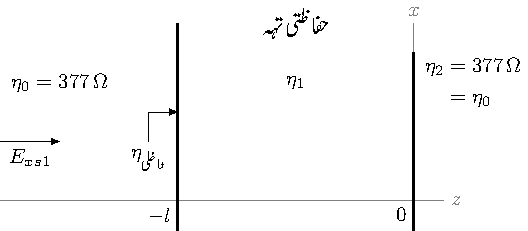
\includegraphics{figWaveRadarAntennaCover}
\caption{ریڈار اینٹینا پر ایسی شفاف حفاظتی تہہ چڑھائی جاتی ہے جو برقی و مقناطیسی امواج کو نہیں گھٹاتی۔}
\label{شکل_موج_ریڈار_اینٹینا_تہہ}
\end{figure}

 ریڈار\فرہنگ{ریڈار}\فرہنگ{radar} اینٹینا\فرہنگ{اینٹینا}\فرہنگ{antenna} کو موسمی اثرات سے بچانے کی خاطر استعمال کئے جانے والی ایسی تہہ کی بات کرتے ہیں جو ریڈار کے شعاعوں کے لئے بالکل شفاف ثابت ہوتی ہے۔یہ تہہ عموماً اینٹینا پر گنبد کی شکل میں ہوتی ہے۔شکل \حوالہ{شکل_موج_ریڈار_اینٹینا_تہہ} میں ریڈار اینٹینا \عددیء{z=-l} کے بائیں جانب خلاء میں ہے جبکہ \عددیء{z=0} تا \عددیء{z=-l} خطے میں حفاظتی تہہ ہے۔یوں \عددیء{z=0} کے دائیں جانب خلاء ہے جس میں ریڈار اشارات بھیجتا ہے۔ خلاء کی قدرتی رکاوٹ \عددیء{\SI{377}{\ohm}} ہوتی ہے۔ذو برق کی بنی حفاظتی تہہ کی موٹائی زیادہ نہیں رکھی جاتی تا کہ اس میں طاقت کا ضیاع کم سے کم ہو۔حفاظتی تہہ سے انعکاس قابل قبول نہیں چونکہ اس طرح ریڈار کے امواج واپس اینٹینا کی طرف لوٹیں گے۔ہم چاہتے ہیں کہ اینٹینا، دائیں جانب کے پورے نظام کے لئے ہم رکاوٹی\فرہنگ{ہم رکاوٹی}\فرہنگ{matched} ہو۔ایسا \عددیء{{\eta_{\text{داخلی}}=\eta_2}} کی صورت میں ہو گا یعنی
\begin{align*}
377=\eta_1 \frac{377+j\eta_1 \tan \beta_1 l}{\eta_1+j 377 \tan \beta_1 l}
\end{align*}
یا
\begin{align*}
j 377^2 \tan \beta_1 l =j \eta_1^2 \tan \beta_1 l
\end{align*}
اب تمام غیر مقناطیسی اشیاء کی \عددیء{\eta_1<377} ہے لہٰذا اس مساوات پر پورا صرف اس صورت اترا جا سکتا ہے جب \عددیء{\beta_1 l =n \pi} ہو۔کم سے کم موٹائی یوں \عددیء{n=1} کی صورت میں \عددیء{l=\tfrac{\pi}{\beta_1}} یعنی \عددیء{l=\tfrac{\lambda_1}{2}} حاصل ہوتی ہے۔اگر ریڈار \عددیء{\SI{10}{\giga\hertz}} کی شعاعیں پیدا کرتا ہو تب ہم حفاظتی تہہ کو کم ضیاع اور ہلکے وزن کے ایسے  پلاسٹک  سے بنا سکتے ہیں جس کا \عددیء{\epsilon_R=2.25} ہے۔ہمیں تہہ کی موٹائی
\begin{align*}
l=\frac{\lambda_1}{2}=\frac{v_1}{2 f_1}=\frac{3\times 10^8}{2 \sqrt{2.25} \times 10^{10}}=\SI{1}{\centi\meter}
\end{align*}
رکھنی ہو گی۔

اگر \عددیء{\SI{10}{\giga\hertz}} پر چلنے والے ریڈار پر چڑھائی حفاظتی تہہ کی موٹائی \عددیء{\SI{0.5}{\centi\meter}} کر دی جائے تب \عددیء{\beta_1=314.2} اور \عددیء{\eta_1=251.33} لیتے ہوئے
\begin{align*}
\eta_{\text{داخلی}}&=251.33 \times \frac{377+j 251.33 \tan (314.2 \times 0.005)}{251.33+j 377 \tan(314.2\times 0.005)}\\
&\approx \SI{167.6}{\ohm}
\end{align*}
ہو گی۔یوں شرح انعکاس
\begin{align*}
\Gamma=\frac{167.6-377}{167.6+377}=-0.3845
\end{align*}
ہو گا اور انعکاسی طاقت کی فی صد شرح
\begin{align*}
\frac{\frac{\left(E_{x10}^-\right)^2}{2\eta_0}}{\frac{\left(E_{x10}^+\right)^2}{2\eta_0}} \times 100=\abs{\Gamma}^2 \times 100=\SI{14.78}{\%}
\end{align*}
ہو گی۔
%===========
\ابتدا{مشق}
دو خطے آپس میں \عددیء{z=0} پر ملتے ہیں۔سرحد کے بائیں جانب پہلا خطہ ہے جس کے مستقل \عددی{\epsilon_{R1}=5}، \عددیء{\mu_{R1}=1} اور \عددیء{\sigma_1=0} ہیں۔سرحد کے دوسری جانب مستقل \عددی{\epsilon_{R2}=2}، \عددیء{\mu_{R2}=10} اور \عددیء{\sigma_2=0} ہیں۔ پہلے خطے میں \عددیء{s} حاصل کریں۔دوسرے خطے میں \عددیء{s} حاصل کریں اور آخر میں \عددیء{z=-\SI{0.6}{\centi\meter}} پر \عددیء{\eta_{\text{داخلی}}} حاصل کریں۔

جوابات:\عددی{5}، \عددیء{1} اور \عددیء{86.9\phase{-61.8^\circ}}
\انتہا{مشق}
%==========
\جزوحصہ{فیبری-پیروٹ طیف پیما}
بصریات کے میدان میں عموماً \اصطلاح{انحرافی مستقل}\فرہنگ{انحرافی مستقل}\حاشیہب{refractive index}\فرہنگ{refractive index} \عددی{n} استعمال کیا جاتا ہے جہاں
\begin{align}
n=\sqrt{\epsilon_R}
\end{align}
کے برابر ہے۔چونکہ \اصطلاح{فیبری-پیروٹ طیف پیما}\فرہنگ{فیبری-پیروٹ طیف پیما}\فرہنگ{پیما!فیبری-پیروٹ طیف}\حاشیہب{Fabry-Perot interferometer}\فرہنگ{Fabry-Perot interferometer}  بصریات میں استعمال کیا جاتا ہے لہٰذا ہم انحرافی مستقل استعمال کرتے ہوئے اس کی کارکردگی پر غور کرتے ہیں۔خالی خلاء میں \عددی{\beta_0=\omega \sqrt{\mu_0 \epsilon_0 }} جبکہ شیشے\حاشیہد{شیشہ غیر مقناطیسی ہے لہٰذا اس کی \عددی{\mu_R=1}=1 ہے۔} میں \عددی{\beta=\omega\sqrt{\mu_0\epsilon_0\epsilon_R}} ہیں۔یوں
\begin{align}
\frac{\lambda_0}{\lambda}=\frac{\beta}{\beta_0}=\sqrt{\epsilon_R}=n
\end{align}
لکھا جا سکتا ہے۔

سادہ ترین صورت میں فیبری-پیروٹ طیف پیما \عددی{n} انحرافی مستقل کے  سادہ شیشے (یا کسی دوسرے شفاف مادے) کا تختہ ہوتا ہے جس کی موٹائی \عددی{l} کو یوں رکھا جاتا ہے کہ درکار طول موج پر یہ مساوات \حوالہ{مساوات_مستوی_دو_سرحدی_ہم_رکاوٹ_شرط}
\begin{align}\label{مساوات_مستوی_فیبری_پیروٹ_الف}
\lambda=\frac{\lambda_0}{n}=\frac{2l}{m} \quad \quad (m=1,2,3\cdots)
\end{align}
 پر پورا اترے جہاں خالی خلاء میں طول موج \عددی{\lambda_0} جبکہ شیشے کے تختے میں طول موج \عددی{\lambda} ہے۔مندرجہ بالا مساوات سے حاصل تمام طول موج، شیشے کے تختے سے بغیر گھٹے گزرتی ہیں۔عموماً ہم چاہتے ہیں کہ شیشے کے تختے سے صرف اور صرف ایک مخصوص طول موج گزر پائے نا کہ ایسے تمام امواج جو مندرجہ بالا مساوات پر پورا اترتے ہوں۔ایسا یوں ممکن بنایا جا سکتا ہے کہ درکار طول موج اور مساوات \حوالہ{مساوات_مستوی_فیبری_پیروٹ_الف} سے حاصل قریبی طول موج میں طویل فاصلہ ہو۔مندرجہ بالا مساوات میں \عددی{m} کی مختلف قیمتیں مختلف طول موج دیتی ہیں۔ایسے دو عدد قریبی طول موج جنہیں اس مساوات میں  \عددی{m} اور \عددی{m-1} پر کرنے سے حاصل کیا گیا ہو میں فرق 
\begin{align}
\lambda_{m-1}-\lambda_m=\Delta \lambda=\frac{2l}{m-1}-\frac{2l}{m}=\frac{2l}{m(m-1)} \approx \frac{2l}{m^2}
\end{align}
ہو گا۔یاد رہے کہ \عددی{m} شیشے میں نصف طول موج کی گنتی
\begin{align}
m=\frac{2l}{\lambda}=\frac{2ln}{\lambda_0}
\end{align}
ہے۔یوں
\begin{align}
\Delta \lambda=\frac{\lambda^2}{2l}
\end{align}
لکھا جا سکتا ہے جسے خالی خلاء میں طول موج \عددی{\lambda_0} کی صورت میں
\begin{align}
\Delta \lambda_0=\frac{\lambda_0^2}{2ln}
\end{align}
لکھا جا سکتا ہے۔درکار طول موج \عددی{\lambda_0} سے قریب تر طول موج، جو شیشے سے گزر پائے گا، کا فاصلہ \عددی{\Delta \lambda_0} ہے جو \اصطلاح{طیفی حد}\فرہنگ{طیفی حد}\فرہنگ{فیبری-پیروٹ!طیفی حد}\حاشیہب{free spectral range}\فرہنگ{free spectral range}\فرہنگ{Fabry-Perot!free spectral range} کہلاتی ہے۔اگر کسی طرح اس فاصلے پر پائے جانے والے  طول موج کو علیحدہ کرنا ممکن ہو تب ہم \عددی{\lambda_0} کو علیحدہ کرنے میں کامیاب ہوں گے۔طیف پیما کو بطور پٹی گزار فلٹر بھی استعمال کیا جا سکتا ہے جہاں درکار طول موج کے قریبی طول موج شیشے سے گزر پاتے ہیں جبکہ اس سے دور طول موج نہیں گزر پاتے۔
%=============== 
\ابتدا{مثال}
سرخ رنگ کی خالی خلاء میں طول موج \عددی{\SI{600}{\nano\meter}} ہے۔ہمیں اس طول موج پر \عددی{\Delta \lambda_0=\SI{100}{\nano\meter}} فاصلے تک طول موج علیحدہ کرنے ہیں۔فیبری-پیروٹ طیف پیما میں استعمال کردہ شیشے کا انحرافی مستقل \عددی{n=1.45} ہے۔شیشے کی موٹائی حاصل کریں۔

حل:ہم چاہیں گے کہ طیف پیما کی \عددی{\Delta \lambda_0} درکار قیمت سے قدر زیادہ ہو یعنی
\begin{align*}
l< \frac{\lambda_0^2}{2n\Delta \lambda_0}=\frac{600\times 10^{-9} \times 600 \times 10^{-9}}{2\times 1.45\times 100 \times 10^{-9}}=\SI{1.241}{\micro\meter}
\end{align*}
\انتہا{مثال}
%===========================

اتنی باریک موٹائی کا شیشہ بنانا یا اسے استعمال کرنا ناممکن سی بات ہے۔اس کا بہتر حل یہ ہو گا کہ دو شیشوں کے درمیان تقریباً یہی فاصلہ رکھا جائے۔ان دو عدد شیشوں کے قریبی سطحوں کے مابین فاصلہ کم یا زیادہ کرتے ہوئے کسی بھی طول موج کو گزارہ جا سکتا ہے۔شیشوں کے بیرونی جانب سطحوں پر \اصطلاح{انعکاس مخالف تہہ}\حاشیہب{antireflective coating} چڑھائی جاتی ہے۔

%=============================
\جزوحصہ{\عددی{\eta_1 \ne \eta_3} کی صورت میں ہم رکاوٹ صورت کا حصول}\شناخت{حصہ_مستوی_دو_سرحدی_ہم_رکاوٹ_عمومی_حل}
اس حصے میں ہم مساوات \حوالہ{مساوات_مستوی_داخلی_رکاوٹ_دو_سرحدی} میں \عددی{\eta_1 \ne \eta_3} کی صورت میں \عددی{\eta_{\text{داخلی}}=\eta_1} کے  حصول پر غور کرتے ہیں جس سے \عددی{\Gamma=0} حاصل ہوتا ہے۔
\begin{align*}
\beta_2 l =(2m-1)\frac{\pi}{2} \quad \quad (m=1,2,3,\cdots)
\end{align*}
یعنی
\begin{align*}
\frac{2\pi}{\lambda_2} l =(2m-1)\frac{\pi}{2} \quad \quad (m=1,2,3,\cdots)
\end{align*}
کی صورت میں 
\begin{align}\label{مساوات_مستوی_بے_انعکاس_الف}
l=(2m-1)\frac{\lambda_2}{4}
\end{align}
لکھا جا سکتا ہے جس کے مطابق دوسرے خطے کی موٹائی، طول موج کے چوتھائی حصے کے طاق گنا ہے۔ایسی صورت میں  مساوات \حوالہ{مساوات_مستوی_داخلی_رکاوٹ_دو_سرحدی} سے
\begin{align}
\eta_{\text{داخلی}}=\frac{\eta_2^2}{\eta_3}
\end{align}
حاصل ہوتا ہے۔ہم دوسرے خطے کی موٹائی کے ذریعہ پہلے خطے کو تیسرے خطے کے ہم رکاوٹ بنا سکتے ہیں۔ایسی صورت میں \عددی{\eta_{\text{داخلی}}=\eta_1} ہو گا لہٰذا مندرجہ بالا مساوات سے
\begin{align}\label{مساوات_مستوی_بے_انعکاس_ب}
\eta_2=\sqrt{\eta_1 \eta_3}
\end{align}
لکھا جا سکتا ہے۔مساوات \حوالہ{مساوات_مستوی_بے_انعکاس_الف} اور مساوات \حوالہ{مساوات_مستوی_بے_انعکاس_ب} \اصطلاح{چوتھائی طول موج}\فرہنگ{چوتھائی طول موج کی ترکیب}\حاشیہب{quarter-wave matching}\فرہنگ{quarter-wave matching} سے ہم رکاوٹ بنانا ممکن بناتا ہے۔ \اصطلاح{انعکاس مخالف تہہ}\فرہنگ{انعکاس مخالف تہہ}\حاشیہب{antireflective coating}\فرہنگ{antireflective coating} کا دارومدار اسی اصول پر ہے۔
%==================
\ابتدا{مثال}
ہم \عددی{\SI{660}{\nano\meter}} طول موج کی شعاع کے لئے \عددی{n_3=1.45} انحرافی مستقل کے شیشے کو خالی خلاء \عددی{n_1=1} کے ہم رکاوٹ بذریعہ انعکاس مخالف تہہ بنانا چاہتے ہیں۔اس تہہ کی کم سے کم موٹائی اور انحرافی مستقل \عددی{n_2} دریافت کریں۔  

حل:خالی خلاء اور شیشے کے قدرتی رکاوٹ
\begin{align*}
\eta_1&=\SI{377}{\ohm}\\
\eta_3&=\frac{377}{1.45}=\SI{260}{\ohm}
\end{align*}
ہیں۔یوں مساوات \حوالہ{مساوات_مستوی_بے_انعکاس_ب} سے انعکاس مخالف تہہ کی قدرتی رکاوٹ
\begin{align*}
\eta_2=\sqrt{377 \times 260}=\SI{313}{\ohm}
\end{align*}
حاصل ہوتی ہے۔یوں تہہ کا انحرافی مستقل
\begin{align*}
n=\frac{377}{313}=1.2
\end{align*}
ہو گا۔دوسرے خطے یعنی ذو برق تہہ میں طول موج
\begin{align*}
\lambda_2=\frac{660}{1.2}=\SI{550}{\nano\meter}
\end{align*}
ہو گا جس سے تہہ کی کم سے کم موٹائی
\begin{align*}
l=\frac{\lambda_2}{4}=\frac{0.1375}{\micro\meter}
\end{align*}
حاصل ہوتی ہے۔
\انتہا{مثال}
%====================
\جزوحصہ{متعدد سرحدی مسئلہ}
ہم تو مختلف خطوں کے درمیان سرحد پر انعکاس کو تفصیلاً دیکھ چکے ہیں۔اسی طرح ہم نے دو سرحدی صورت حال پر بھی غور کیا۔آئیں اس حصے میں متعدد سرحدی صورت میں شرح انعکاس حاصل کریں۔شکل \حوالہ{شکل_مستوی_متعدد_سرحدی_شرح_انعکاس} میں تین سرحدی مسئلہ دکھایا گیا ہے جس پر غور کرتے ہوئے متعدد سرحدی مسئلے کا حل تلاش کیا جائے گا۔

\begin{figure}
\centering
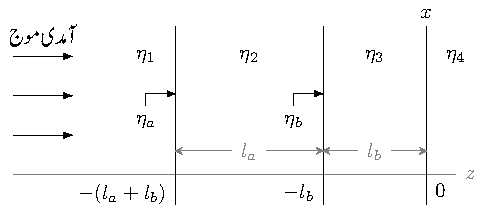
\includegraphics{figWaveMultipleBoundaryReflection}
\caption{متعدد سرحدی صورت میں شرح انعکاس۔}
\label{شکل_مستوی_متعدد_سرحدی_شرح_انعکاس}
\end{figure}

ہمیں آمدی طاقت کا وہ حصہ دریافت کرنا ہے جو تین سرحدی تہہ سے گزر نہیں پاتا بلکہ یہ انعکاس پذیر ہو کر آمدی موج کے الٹ سمت میں واپس چلے جاتا ہے۔اسی طرح ہمیں آمدی طاقت کا وہ حصہ دریافت کرنا ہے جو تینوں سرحدوں کو عبور کرتے ہوئے چوتھے خطے میں ترسیل کر پاتا ہے۔ایسا کرنے کی خاطر ہمیں پہلی سرحد پر داخلی قدرتی رکاوٹ \عددی{\eta_a}  درکار ہو گی۔مسئلے کو حل کرنے کی خاطر ہمیں اختتامی سرحد سے ابتدائی سرحد کی جانب چلتے ہوئے  ہر سرحد پر داخلی قدرتی رکاوٹ حاصل کرنے ہوں گے۔یوں ہم پہلے \عددی{\eta_b} حاصل کریں گے۔یوں تیسرے اور چوتھے خطے کے اثرات کو \عددی{\eta_b} سے ظاہر کرتے ہوئے ہم پہلی سرحد پر پہنچیں گے۔

مساوات \حوالہ{مساوات_مستوی_داخلی_رکاوٹ_دو_سرحدی} استعمال کرتے ہوئے
\begin{align}
\eta_{b}= \eta_3 \frac{\eta_4 \cos \beta_3 l_b +j \eta_3 \sin \beta_3 l_b}{\eta_3 \cos \beta_3 l_b +j \eta_4\sin \beta_3 l_b}
\end{align}
لکھا جا سکتا ہے۔اس طرح ہم \اصطلاح{تبادلہ رکاوٹ}\فرہنگ{تبادلہ رکاوٹ}\حاشیہب{impedance transformation}\فرہنگ{impedance transformation} کی مدد سے تین سرحدی مسئلے کو دو سرحدی مسئلہ بنا پائے ہیں جہاں دوسری سرحد کے دائیں جانب جو کچھ بھی ہے اسے \عددی{\eta_b} سے ظاہر کیا جاتا ہے۔اب پہلے سرحد پر مساوات \حوالہ{مساوات_مستوی_داخلی_رکاوٹ_دو_سرحدی} کے استعمال سے
 \begin{align}
\eta_{a}= \eta_2 \frac{\eta_b \cos \beta_2 l_a +j \eta_2 \sin \beta_2 l_a}{\eta_2 \cos \beta_2 l_a +j \eta_b\sin \beta_2 l_a}
\end{align}
لکھا جا سکتا ہے۔

آمدی طاقت کا \عددی{\Gamma^2} حصہ انعکاسی طاقت ہو گا جہاں
\begin{align}
\Gamma=\frac{\eta_a-\eta_1}{\eta_a+\eta_1}
\end{align}
کے برابر ہے۔آمدی طاقت کا بقایا حصہ یعنی \عددی{1-\Gamma^2} حصہ چوتھے خطے میں ترسیل ہو گا۔ تبادلہ رکاوٹ کی ترکیب متعدد سرحدی مسئلے پر لاگو کیا جا سکتا ہے۔

کیمرے\فرہنگ{کیمرہ}\حاشیہب{camera}\فرہنگ{camera} کے عدسہ\فرہنگ{عدسہ}\حاشیہب{lens}\فرہنگ{lens} پر متعدد تہہ چڑھا کر اس کی کارکردگی بہتر کی جاتی ہے۔یوں عدسہ پر پہلی تہہ کا انحرافی مستقل عدسے کے شیشے کے انحرافی مستقل کے برابر ہو گا۔اگلی تہہ کا انحرافی مستقل قدر کم ہو گا۔اسی طرح آخری تہہ کا انحرافی مستقل عین خالی خلاء کے انحرافی مستقل کے برابر ہو گا۔یوں ایک تہہ سے دوسرے تہہ میں موج بغیر انعکاس کے داخل ہو گی۔موج کو سرحد نظر ہی نہیں آتا۔  
%=========================
\حصہ{خطی، بیضوی اور دائری تقطیب}
اس حصے میں \اصطلاح{تقطیب موج}\فرہنگ{تقطیب موج}\فرہنگ{موج!تقطیب}\حاشیہب{wave polarization}\فرہنگ{wave!polarization}  پر غور کیا جائے گا۔خطی تقطیب اور بیضوی تقطیب کے بعد دائری تقطیب پر تبصرہ کیا جائے گا۔

اب تک اٹل سمت کے امواج پر غور کیا گیا۔یوں \عددیء{\az} جانب حرکت کرتا \عددیء{\ax} سمت کا میدان
\begin{align}
E_x = E_{x0} \cos (\omega t -\beta z)
\end{align}
لکھا گیا۔یہ مساوات خطی تقطیب کی مثال ہے جہاں میدان تمام اوقات صرف \عددیء{x} سمت میں پایا جاتا ہے۔عموماً \عددیء{\az} جانب حرکت کرتے موج میں \عددیء{\ax} کے علاوہ \عددیء{\ay} جزو بھی پایا جائے گا۔ایسی صورت میں موج کے اجزاء
\begin{gather}
\begin{aligned}\label{مساوات_قطبیت_عمومی_اجزاء}
E_x&=E_1 \cos (\omega t -\beta z)\\
E_y&=E_2 \cos (\omega t -\beta z -\delta)
\end{aligned}
\end{gather}
ہو سکتے ہیں جہاں دونوں اجزاء کے حیطے مختلف ممکن ہیں جبکہ ان میں زاویائی فاصلہ \عددیء{\delta} بھی پایا جا سکتا ہے۔ان اجزاء کا مجموعہ
\begin{align}\label{مساوات_قطبیت_عمومی_مساوات}
\kvec{E}=E_1 \cos (\omega t -\beta z) \ax+E_2 \cos (\omega t -\beta z -\delta) \ay
\end{align}
ایسی موج کو ظاہر کرے گا۔یہ مساوات غور طلب ہے۔آئیں خلاء میں کسی بھی اٹل نقطے پر وقت تبدیل ہونے سے  ایسی میدان پر غور کریں۔ہم خلاء میں  \عددیء{z=0} کو اٹل نقطہ لیتے ہوئے  میدان حاصل کرتے ہیں۔

\begin{figure}
\centering
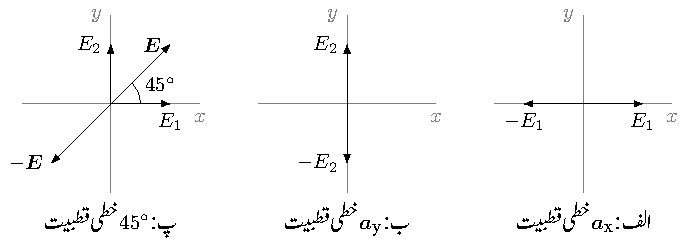
\includegraphics{figPolarizationFieldDirections}
\caption{خطی، دائری اور بیضوی قطبیت۔}
\label{شکل_قطبیت_خطی_قطبیت}
\end{figure}
اگر \عددیء{E_2=0} ہو تب وقت \عددیء{t} کے تبدیلی سے میدان کی قیمت \عددیء{-E_1\ax} تا \عددیء{+E_1\ax} تبدیل ہوتی ہے۔اس میدان کو تمام \عددیء{t} کے لئے شکل \حوالہ{شکل_قطبیت_خطی_قطبیت}-الف میں دکھایا گیا ہے۔آپ دیکھ سکتے ہیں کہ میدان کی نوک \عددیء{-E_1} تا \عددیء{+E_1} خطی لکیر پر رہتی ہے۔اسی حقیقت سے ایسے موج کی قطبیت کو \اصطلاح{خطی قطبیت}\فرہنگ{خطی!قطبیت}\فرہنگ{ْقطبیت!خطی}\حاشیہب{linear polarization}\فرہنگ{linear polarization}\فرہنگ{polarization!linear}\فرہنگ{linear!polarization}  کہتے ہیں۔یہ موج \عددیء{\ax} سمت میں خطی قطبیت رکھتی ہے۔اس کے برعکس اگر مساوات \حوالہ{مساوات_قطبیت_عمومی_مساوات} میں \عددیء{E_1=0} ہو تب یہ \عددیء{\ay} خطی قطبیت کی موج ہو گی جسے شکل \حوالہ{شکل_قطبیت_خطی_قطبیت}-ب میں دکھایا گیا ہے۔اگر \عددیء{E_1=E_2=E_{12}} اور \عددیء{\delta=0} ہوں تب بھی خطی قطبیت کی موج حاصل ہوتی ہے البتہ یہ موج افقی محدد کے ساتھ \عددیء{45^\circ} کا زاویہ بناتی ہے۔شکل \حوالہ{شکل_قطبیت_خطی_قطبیت}-پ میں اس موج کو دکھایا گیا ہے۔

آئیں اب ذرہ دلچسپ صورت حال دیکھیں۔نقطہ \عددیء{z=0} پر مساوات \حوالہ{مساوات_قطبیت_عمومی_اجزاء}
\begin{gather}
\begin{aligned}\label{مساوات_قطبیت_ابتدائی_نقطے_پر_میدان}
E_x&=E_1 \cos \omega t\\
E_y&=E_2 \cos (\omega t  -\delta)
\end{aligned}
\end{gather}
صورت اختیار کر لیتے ہیں جس میں \عددیء{E_y} کو
\begin{align*}
E_y=E_2 \left(\cos \omega t \cos \delta + \sin \omega t \sin \delta\right)
\end{align*}
لکھنا ممکن ہے۔اس مساوات میں،  \عددیء{E_x} کی مساوات استعمال کرتے ہوئے،  \عددیء{\cos \omega t =\tfrac{E_x}{E_1}} اور \عددیء{\sin \omega t=\sqrt{1-\left(\tfrac{E_x}{E_1} \right)^2}} پر کر کے
\begin{align*}
E_y=E_2 \left[\frac{E_x}{E_1} \cos \delta+\sqrt{1-\left(\frac{E_x}{E_1}\right)^2} \sin \delta\right]
\end{align*}
ملتا ہے جسے
\begin{align}\label{مساوات_قطبیت_عمومی_بیضوی_قطبیت_الف}
\frac{E_x^2}{E_1^2}-2 \frac{E_x}{E_1} \frac{E_y}{E_2} \cos \delta +\frac{E_y^2}{E_2^2}=\sin^2 \delta
\end{align}
یا
\begin{align}\label{مساوات_قطبیت_عمومی_بیضوی_قطبیت_ب}
a E_x^2-b E_x E_y +c E_y^2=1
\end{align}
لکھا جا سکتا ہے جہاں
\begin{align}
a=\frac{1}{E_1^2 \sin^2 \delta} \quad \quad b=\frac{2 \cos \delta}{E_1 E_2 \sin^2 \delta} \quad \quad c=\frac{1}{E_2^2 \sin^2 \delta}
\end{align}
لئے گئے ہیں۔مساوات \حوالہ{مساوات_قطبیت_عمومی_بیضوی_قطبیت_ب} \اصطلاح{بیضوی قطبیت}\فرہنگ{قطبیت!بیضوی}\فرہنگ{بیضوی قطبیت}\حاشیہب{elliptic polarization}\فرہنگ{elliptic!polarization}\فرہنگ{polarization!elliptic} کی عمومی مساوات ہے۔

مساوات \حوالہ{مساوات_قطبیت_عمومی_بیضوی_قطبیت_الف} میں \عددیء{E_1=E_2=E_{0}} اور \عددیء{\delta=\mp 90^\circ} کی صورت میں
\begin{align}\label{مساوات_قطبیت_عمومی_دائری_قطبیت}
E_x^2 +E_y^2=E_{0}^2
\end{align}
حاصل ہوتا ہے جو دائرے کی مساوات ہے اور جسے شکل \حوالہ{شکل_قطبیت_دائری_اور_بیضوی_قطبیت}-الف میں دکھایا گیا ہے۔شکل میں \عددیء{E_1} اور \عددیء{E_2} بھی ظاہر کئے گئے ہیں جن کی لمبائی برابر ہے۔مساوات \حوالہ{مساوات_قطبیت_ابتدائی_نقطے_پر_میدان} سے \عددیء{\delta=+90^\circ} کی صورت میں \عددیء{\omega t=0} پر 
\begin{align*}
E_x&=E_{0} \cos 0=E_{0}\\  
E_y&=E_{0} \cos (0  -90^\circ) =0  \quad \quad (\delta =+90^\circ)
\end{align*}
حاصل ہوتے ہیں جبکہ کچھ ہی لمحے بعد \عددیء{\omega t =30^\circ} کی صورت میں
\begin{align*}
E_x&=E_{0} \cos 30^\circ=0.866 E_{0} \\
E_y&=E_{0} \cos (30^\circ  -90^\circ) =0.5 E_{0} \quad \quad (\delta =+90^\circ)
\end{align*}
حاصل ہوتا ہے۔شکل \حوالہ{شکل_قطبیت_دایاں_بایاں_ہاتھ_دائری}-الف میں دونوں اوقات پر موج دکھائی گئی ہے۔آپ دیکھ سکتے ہیں کہ بڑھتے وقت کے ساتھ میدان کی نوک دائرے پر گھڑی کے الٹ سمت میں حرکت کرتی ہے۔اس شکل میں موج کے حرکت کی سمت \عددیء{\az} کاغذ سے باہر کو ہے۔اگر دائیں ہاتھ کے انگوٹھے کو موج کے حرکت کی سمت میں رکھا جائے تو اس ہاتھ کی بقایا چار انگلیاں دائرے پر میدان کی نوک کی حرکت کا سمت دیتی ہیں۔یوں \عددیء{\delta=+90^\circ} کی صورت میں مساوات \حوالہ{مساوات_قطبیت_عمومی_دائری_قطبیت} \اصطلاح{دائیں دائری قطبیت}\فرہنگ{دایاں دائری قطبیت}\فرہنگ{قطبیت!دایاں دائری}\حاشیہب{right circular polarization}\فرہنگ{right circular polarization}\فرہنگ{polarization!right circular} کی موج کو ظاہر کرتا ہے۔   
\begin{figure}
\centering
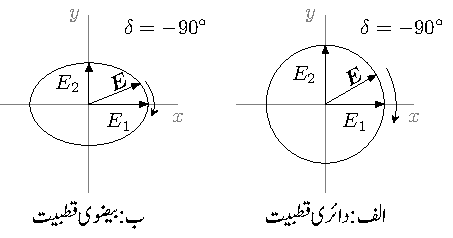
\includegraphics{figPolarizationCircularAndElliptic}
\caption{دائری اور بیضوی قطبیت۔}
\label{شکل_قطبیت_دائری_اور_بیضوی_قطبیت}
\end{figure}

اسی طرح \عددیء{\delta=-90^\circ} کی صورت میں \اصطلاح{بائیں دائری قطبیت}\فرہنگ{قطبیت!بائیں دائری}\حاشیہب{left circular polarization}\فرہنگ{left circular polarization} حاصل ہوتی ہے جسے شکل \حوالہ{شکل_قطبیت_دایاں_بایاں_ہاتھ_دائری}-ب میں دکھایا گیا ہے۔

دائیں ہاتھ قطبی موج سے مراد وہ موج ہے جو آپ کی طرف حرکت کرتے ہوئے آپ کو گھڑی کے الٹ گھومتی نظر آئے۔کسی موج کی قطبیت سے مراد وہ قطبیت ہے جو دیکھنے والے کی طرف حرکت کرتی موج کی قطبیت ہو گی۔

جہاں بھی غلطی کی گنجائش ہو وہاں بہتر ہوتا ہے کہ قطبیت کا ذکر کرتے وقت حرکت کی سمت کا بھی ذکر کیا جائے۔

\begin{figure}
\centering
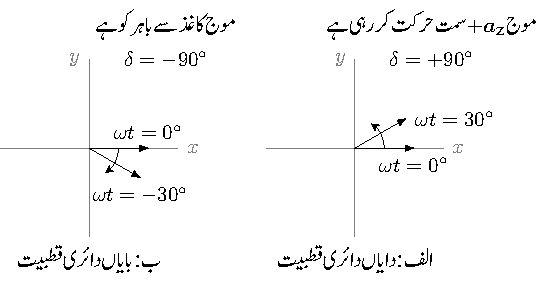
\includegraphics{figPolarizationRightAndLeftCircularPolarizeds}
\caption{دائیں ہاتھ اور بائیں ہاتھ کی دائری قطبیت۔}
\label{شکل_قطبیت_دایاں_بایاں_ہاتھ_دائری}
\end{figure}

مساوات \حوالہ{مساوات_قطبیت_عمومی_بیضوی_قطبیت_الف} میں \عددی{\delta=\mp 90^{\circ}} اور \عددیء{E_1 \ne E_2} کی صورت میں بیضوی موج حاصل ہوتی ہے جسے شکل \حوالہ{شکل_قطبیت_دائری_اور_بیضوی_قطبیت}-ب میں دکھایا گیا ہے۔

شکل \حوالہ{شکل_قطبیت_عمومی_بیضوی} میں مساوات \حوالہ{مساوات_قطبیت_عمومی_بیضوی_قطبیت_الف} کی عمومی شکل دکھائی گئی ہے جس میں \عددی{\delta \ne 90^{\circ}} اور \عددیء{E_1 \ne E_2}  ہیں۔
\begin{figure}
\centering
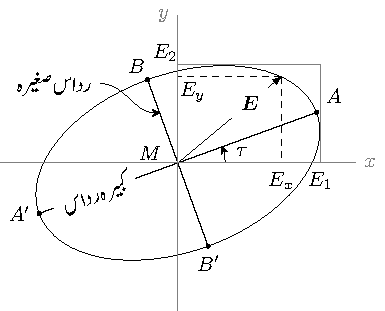
\includegraphics{figPolarizationEllipticAtAngle}
\caption{عمومی بیضوی قطبیت۔}
\label{شکل_قطبیت_عمومی_بیضوی}
\end{figure}
اس شکل میں \اصطلاح{ترخیم}\فرہنگ{ترخیم}\حاشیہب{ellipse}\فرہنگ{ellipse} افقی محدد کے ساتھ \عددیء{\tau} زاویہ بناتا ہے۔یوں \عددی{\tau=15^{\circ}} کی صورت میں یہ  \عددی{15^{\circ}} قطبی موج کہلائے گی۔ شکل \حوالہ{شکل_قطبیت_عمومی_بیضوی} میں رداس کبیرہ \عددی{MA} اور رداس صغیرہ \عددی{MB} کی شرح کو \اصطلاح{شرح رداس}\فرہنگ{شرح رداس}\حاشیہب{axial ratio}\فرہنگ{axial ratio}
\begin{align}
\text{\RL{شرح رداس}}=\frac{AA'}{BB'}
\end{align}
 کہا جاتا ہے جبکہ \عددی{\tau} موج کا \اصطلاح{زاویہ جھکاو}\فرہنگ{زاویہ جھکاو}\حاشیہب{tilt angle}\فرہنگ{tilt angle} کہلاتا ہے۔\عددی{AA'} محور کبیرہ اور \عددی{BB'} محور صغیرہ کہلاتے ہیں۔
%=========================
\ابتدا{مثال}\شناخت{مثال_قطبیت_بیضوی}
برقی موج \عددی{\kvec{E}=3\cos(\omega t-\beta z -45^{\circ}) \ax-4\cos(\omega t -\beta z+30^{\circ})\ay} کا شرح رداس اور \عددی{z=0} پر زاویہ جھکاو حاصل کریں۔

حل:پہلے موج کا زیادہ سے زیادہ حیطہ اور کم سے کم حیطہ دریافت کرتے ہیں۔کسی بھی تفاعل \عددی{f(x)} کی زیادہ سے زیادہ یا کم سے کم قیمت دریافت کرنے کی خاطر پہلے وہ نقطہ \عددی{x_0} دریافت کیا جاتا ہے جہاں درکار قیمت پائی جائے گی۔یہ نقطہ \عددی{\tfrac{\dif f}{\dif x}=0} سے حاصل ہوتا ہے۔

دی گئی برقی موج کی عمومی صورت
\begin{align}
\kvec{E}=E_x \cos \theta+E_y\cos(\theta+\delta)
\end{align}
ہے جس سے
\begin{align*}
\abs{\kvec{E}}^2=E_x^2 \cos^2 \theta +E_y^2 \cos^2(\theta+\delta)
\end{align*}
لکھا جا سکتا ہے۔ہمیں متغیرہ \عددی{\theta} کی وہ قیمت درکار ہے جس پر \عددی{\abs{\kvec{E}}^2} زیادہ سے زیادہ یا کم سے کم پایا جائے گا۔اس تفاعل کا تفرق صفر کے برابر پر کرتے ہیں۔
\begin{align*}
-2 E_x^2 \cos \theta \sin \theta -2 E_y^2 \cos(\theta+\delta) \sin(\theta+\delta)=0 
\end{align*}
اس میں \عددی{\sin 2\alpha=2\sin\alpha\cos\alpha} استعمال کرتے  ہوئے یوں لکھا جا سکتا ہے۔
\begin{align*}
E_x^2 \sin 2\theta+E_y^2 \sin[2(\theta+\delta)]=0
\end{align*}
اب \عددی{\sin(2\theta+2\delta)=\sin 2\theta \cos 2\delta+\cos 2\theta\sin 2\delta} پر کرتے ہیں۔
\begin{align*}
E_x^2 \sin 2\theta +E_y^2 [\sin 2 \theta \cos 2 \delta +\cos 2 \theta \sin 2 \delta]=0
\end{align*}
اس سے یوں لکھا جا سکتا ہے
\begin{align*}
\tan 2 \theta =\frac{\sin 2 \theta}{\cos 2 \theta}=\frac{-E_y^2 \sin 2 \delta}{E_x^2+E_y^2 \cos 2 \delta}
\end{align*}
جس سے
\begin{align}\label{مساوات_قطبیت_رداس_الف}
\theta_{01}=\frac{1}{2} \tan^{-1}\left( \frac{-E_y^2 \sin 2 \delta}{E_x^2+E_y^2 \cos 2 \delta}\right)
\end{align}
حاصل ہوتا ہے۔محور کبیرہ اور محور صغیرہ میں \عددی{90^{\circ}} کا فرق پایا جاتا ہے لہٰذا دوسرا محور
\begin{align}\label{مساوات_قطبیت_رداس_ب}
\theta_{02}=90^{\circ}+\theta_{01}
\end{align}
پر ہو گا۔ان میں ایک نقطے پر تفاعل کی کم سے کم قیمت حاصل ہو گی جبکہ دوسرے نقطے پر تفاعل کی زیادہ سے زیادہ قیمت حاصل ہو گی۔

سوال میں دی گئی موج میں \عددی{\omega t -\beta z-45^{\circ}=\theta} پر کرنے سے اسے
\begin{align*}
\kvec{E}=3\cos \theta-4\cos (\theta+75^{\circ})
\end{align*}
لکھا جا سکتا ہے۔یوں مساوات \حوالہ{مساوات_قطبیت_رداس_الف} اور مساوات \حوالہ{مساوات_قطبیت_رداس_ب} سے
\begin{align*}
\theta_{01}&=\omega t -\beta z -45^{\circ}=\frac{1}{2} \tan^{-1}\left( \frac{-(-4)^2 \sin (2 \times 75^{\circ})}{3^2+(-4^2 \cos (2 \times 75^{\circ})}\right)=29.37^{\circ}\\
\theta_{02}&=90^{\circ}+29.37=119.37^{\circ}
\end{align*}
حاصل ہوتے ہیں۔پہلے نقطے پر محور
\begin{align*}
\kvec{E}&=3\cos 29.37^{\circ} \ax -4 \cos (29.37^{\circ}+75^{\circ}) \ay\\
&=2.6144\ax+0.9927\ay\\
&=2.797 \phase{20.792^{\circ}}
\end{align*}
جبکہ دوسرے نقطے پر محور
\begin{align*}
\kvec{E}&=-1.471\ax+3.875\ay\\
&=4.145\phase {110.79^{\circ}}
\end{align*}
پایا جائے گا۔دوسرے محور کی لمبائی زیادہ ہے لہٰذا یہ محور کبیرہ ہے۔ شرح رداس
\begin{align*}
\frac{4.145}{2.797}=1.42
\end{align*}
ہے جبکہ محور کبیرہ کا زاویہ جھکاو \عددی{110.79^{\circ}} یا \عددی{-69.11^{\circ}} دیتا ہے۔شکل \حوالہ{شکل_قطبیت_مثال_بیضوی} میں نتائج دکھائے گئے ہیں۔
\begin{figure}
\centering
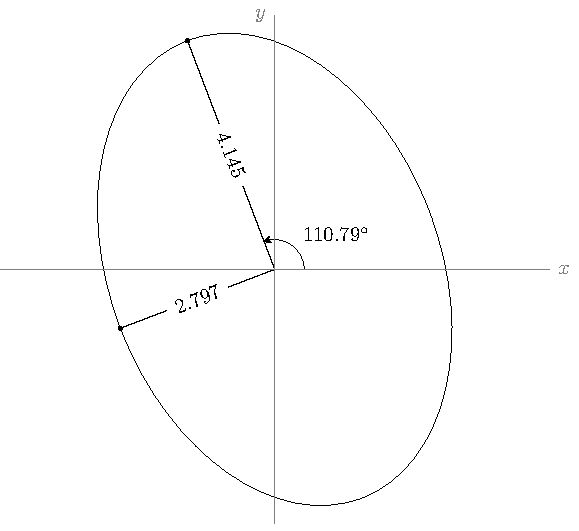
\includegraphics{figPolarizationEllipticAtAngleExample}
\caption{مثال  \حوالہ{مثال_قطبیت_بیضوی} کی بیضوی قطبی موج۔}
\label{شکل_قطبیت_مثال_بیضوی}
\end{figure}
\انتہا{مثال}
%========================
\ابتدا{مثال}
صفحہ کتاب کے عمودی باہر کی جانب موج کے اجزاء \عددی{E_x=5\cos \omega t} اور \عددی{E_y=15\cos(\omega t +90^{\circ})} ہیں۔موج کی شرح رداس، تقطیب اور زاویہ جھکاو حاصل کریں۔

حل:
\begin{align*}
\text{\RL{شرح رداس}}=\frac{15}{5}=3
\end{align*}
کبیرہ اور صغیرہ رداس برابر نہ ہونے کی وجہ سے بیضوی موج پائی جائے گی۔گھومنے کی سمت دریافت کرنے کی خاطر ہم کسی بھی دو قریبی لمحات پر موج کو دیکھتے ہیں۔یوں لمحہ \عددی{\omega t =0} پر 
\begin{align*}
E_x&=5 \cos 0^{\circ}=5\\
E_y&=15\cos 90^{\circ}=0
\end{align*}
ہوں گے جبکہ \عددی{\omega t =30^{\circ}} پر
\begin{align*}
E_x&=5 \cos 30^{\circ}=4.33\\
E_y&=15\cos(30^\circ+90^{\circ})=-7.5
\end{align*}
ہوں گے۔ان نتائج سے صاف ظاہر ہے کہ موج گھڑی کی سمت گھوم رہی ہے لہٰذا یہ بائیں بیضوی قطبی موج کہلائے گی۔

چونکہ کبیرہ رداس \عددی{y} محدد جبکہ صغیرہ رداس \عددی{x} محدد پر ہیں لہٰذا زاویہ جھکاو \عددی{90^{\circ}} ہے۔ 
\انتہا{مثال}
%======================
\ابتدا{مثال}\شناخت{مثال_مستوی_دایاں_دائری_قطبی}
موج کی دوری سمتی مساوات \عددی{\kvec{E}_s=E_0(\ax-j\ay)e^{-j\beta z}} ہے۔موج کی حقیقی مساوات حاصل کرتے ہوئے اس کی قطبیت دریافت کریں۔

حل:موج کو حقیقی شکل میں لکھنے کی خاطر دوری سمتی مساوات کو \عددی{e^{j\omega t}} سے ضرب دیتے ہوئے  یولر مماثل کا استعمال کرتے ہیں۔
\begin{align*}
\kvec{E}&=E_0(\ax-j\ay)e^{j(\omega t -\beta z)}\\
&=E_0(\ax-j\ay)[\cos(\omega t -\beta z)+j \sin(\omega t -\beta z)]\\
&=E_0 [\ax \cos (\omega t -\beta z)+\ay \sin(\omega t -\beta z)]+j E_0[\ax \sin(\omega t -\beta z)-\ay \cos(\omega t -\beta z)]
\end{align*}
اس کا حقیقی جزو 
\begin{align*}
\kvec{E}=E_0 [\ax \cos (\omega t -\beta z)+\ay \sin(\omega t -\beta z)]
\end{align*}
یعنی
\begin{align}\label{مساوات_قطبیت_دائیں_دائری_کوسائن}
\kvec{E}=E_0[\ax \cos(\omega t-\beta z)+\ay \cos(\omega t -\beta z -90^{\circ})] \quad \text{\RL{دایاں دائری قطبی}}
\end{align}
ہے جو حقیقی موج کی مساوات ہے۔

کسی بھی نقطے مثلاً \عددی{z=0} پر دو قریبی لمحات پر موج کو دیکھتے ہوئے، اس کے گھومنے کی سمت دیکھی جا سکتی ہے۔لمحہ \عددی{\omega t =0} پر موج \عددی{\ax} سمت میں ہے جبکہ لمحہ \عددی{\omega t =90^{\circ}} پر موج \عددی{\ay} سمت میں ہے۔یوں موج الٹ گھڑی گھوم رہی ہے۔چونکہ رداس کبیرہ اور رداس صغیرہ برابر ہیں لہٰذا یہ دائری موج ہے۔ اس موج کو دائیں دائری قطبی موج کہا جائے گا۔سوال \حوالہ{سوال_قطبی_بائیں_دائری_قطبی_موج} میں آپ سے گزارش کی گئی ہے کہ بایاں دائری قطبی موج کی مساوات
\begin{align}\label{مساوات_قطبیت_بائیں_دائری_کوسائن}
\kvec{E}=E_0[\ax \cos(\omega t-\beta z)+\ay \cos(\omega t -\beta z +90^{\circ})] \quad \text{\RL{بایاں دائری قطبی}}
\end{align}
 حاصل کریں۔
\انتہا{مثال}
%============================
\ابتدا{مشق}
موج کی دوری سمتی مساوات \عددی{\kvec{E}_s=E_0(\ax-j\ay)e^{j\beta z}} ہے۔موج کی حقیقی مساوات حاصل کرتے ہوئے اس کی قطبیت دریافت کریں۔

جواب:دھیان رہے کہ یہ موج منفی \عددی{z} محدد کی جانب حرکت کر رہی ہے۔یوں یہ بائیں دائری قطبی موج ہے۔ 
\انتہا{مشق}
%===============================
\ابتدا{مثال}
دائیں دائری قطبی موج \عددی{E_0(\ax-j\ay)e^{-j\beta z}} اور بائیں دائری قطبی موج \عددی{E_0(\ax+j\ay)e^{-j\beta z}e^{j\delta}} میں \عددی{\delta} زاویائی فرق پایا جاتا ہے۔ان کا مجموعہ دریافت کریں۔


حل:ان کا مجموعہ
\begin{align*}
\kvec{E}&=E_0 (\ax-j\ay)e^{-j\beta z}+E_0(\ax+j\ay)e^{-j\beta z} e^{j\delta}\\
&=E_0[(1+e^{j\delta})\ax-j(1-e^{j\delta})\ay]e^{-j\beta z}
\end{align*}
ہو گا۔اس سے \عددی{e^{j\tfrac{\delta}{2}}} باہر نکالتے ہوئے
\begin{align*}
\kvec{E}=E_0 e^{j\frac{\delta}{2}}[(e^{-j\frac{\delta}{2}}+e^{j\frac{\delta}{2}})\ax-j(e^{-j\frac{\delta}{2}}-e^{j\frac{\delta}{2}})\ay]e^{-j\beta z}
\end{align*}
لکھا جا سکتا ہے جس میں \عددی{e^{j\tfrac{\delta}{2}}+e^{j\tfrac{\delta}{2}}=2\cos\tfrac{\delta}{2}} اور
 \عددی{e^{j\tfrac{\delta}{2}}-e^{j\tfrac{\delta}{2}}=j 2\sin\tfrac{\delta}{2}} پر کرنے سے
\begin{align}\label{مساوات_تقطیب_دائری_سے_خطی}
\kvec{E}=2 E_0 \left[\cos \left(\frac{\delta}{2}\right) \ax+\sin \left(\frac{\delta}{2}\right)\ay\right]e^{-j(\beta z-\frac{\delta}{2})}
\end{align}
حاصل ہوتا ہے۔مساوات \حوالہ{مساوات_تقطیب_دائری_سے_خطی} خطی قطبی موج ہے جو \عددی{x} محدد کے ساتھ \عددی{\tfrac{\delta}{2}} زاویے پر ہے۔اس مثال سے ثابت ہوا کہ کسی بھی خطی قطبی موج کو دو عدد دائری قطبی امواج کا مجموعی تصور کیا جا سکتا ہے۔
\انتہا{مثال}
%=============================
\حصہ{بیضوی یا دائری قطبی امواج کا پوئنٹنگ سمتیہ}
کسی بھی موج کی اوسط طاقت مساوات \حوالہ{مساوات_موج_مخلوط_پوئنٹنگ_سمتیہ}
\begin{align*}
\pmb{\mathscr{P}}_{\text{اوسط}}=\frac{1}{2}\left[\kvec{E}_s \times \kvec{H}_s^* \right]_{\text{حقیقی}}
\end{align*}
سے حاصل کی جا سکتی ہے۔شکل \حوالہ{شکل_قطبیت_عمومی_بیضوی} کے عمومی بیضوی قطبی موج کے \عددی{x} اور \عددیء{y} اجزاء
\begin{align}
E_{sx}&=E_1 e^{j(\omega t -\beta z)} \label{مساوات_تقطیب_عمومی_بیضوی_برقی_الف}\\
E_{sy}&=E_2 e^{j(\omega t -\beta z +\delta)}\label{مساوات_تقطیب_عمومی_بیضوی_برقی_ب}
\end{align}
میں \عددیء{\delta} زاویائی فرق پایا جاتا ہے۔کسی بھی نقطے پر کل برقی میدان ان اجزاء کا سمتی مجموعہ ہو گا جسے نقطہ \عددیء{z=0} پر 
\begin{align}
\kvec{E}_s =\ax E_1 e^{j \omega t}+\ay E_2 e^{j(\omega t +\delta)}
\end{align}
لکھا جا سکتا ہے۔چونکہ
\begin{align*}
\frac{\kvec{E}}{\kvec{H}}=\eta=\abs{\eta}e^{j \theta_{\eta}}
\end{align*}
ہوتا ہے لہٰذا مساوات \حوالہ{مساوات_تقطیب_عمومی_بیضوی_برقی_الف} کی جوڑی مقناطیسی موج
\begin{align*}
H_{sy}=\frac{E_{sx}}{\abs{\eta}} e^{-j \theta_{\eta}}=\frac{E_1}{\abs{\eta}} e^{j(\omega t -\beta z-\theta_{\eta})}=H_1 e^{j(\omega t -\beta z-\theta_{\eta})}
\end{align*}
ہو گی۔اسی طرح مساوات \حوالہ{مساوات_تقطیب_عمومی_بیضوی_برقی_ب} کی جوڑی
\begin{align}
H_{sx}=-H_2 e^{j(\omega t -\beta z+\delta-\theta_{\eta})}
\end{align}
ہو گی۔کسی بھی نقطے پر مقناطیسی میدان ان اجزاء کا سمتی مجموعہ ہو گا جسے نقطہ \عددیء{z=0} پر
\begin{align}
\kvec{H}_s=-\ax H_2 e^{j(\omega t +\delta-\theta_{\eta})}+\ay H_1 e^{j(\omega t -\theta_{\eta})}
\end{align}
لکھا جا سکتا ہے۔جوڑی دار مخلوط \عددیء{\kvec{H}_s} کی قیمت مندرجہ بالا مساوات میں مثبت \عددیء{j} کو منفی اور منفی \عددیء{j} کو مثبت لکھ کر حاصل ہوتا ہے یعنی
\begin{align}
\kvec{H}_s^*=-\ax H_2 e^{-j(\omega t +\delta-\theta_{\eta})}+\ay H_1 e^{-j(\omega t -\theta_{\eta})}
\end{align}
مخلوط پوئنٹنگ سمتیہ سے اوسط طاقت
\begin{align*}
\pmb{\mathscr{P}}_{\text{اوسط}}&=\frac{1}{2}\left[\left(\ax E_1 e^{j \omega t}+\ay E_2 e^{j(\omega t +\delta)}\right) \times \left(-\ax H_2 e^{-j(\omega t +\delta-\theta_{\eta})}+\ay H_1 e^{-j(\omega t -\theta_{\eta})}\right) \right]_{\text{حقیقی}}\\
&=\frac{1}{2} \az \left[E_1 H_1 e^{j\theta_{\eta}}+E_2 H_2 e^{j \theta_{\eta}} \right]_{\text{حقیقی}}
\end{align*}
یعنی
\begin{align}
\pmb{\mathscr{P}}_{\text{اوسط}}&=\frac{1}{2} \az \left(E_1 H_1+E_2 H_2 \right) \cos \theta_{\eta}
\end{align}
حاصل ہوتی ہے۔آپ دیکھ سکتے ہیں کہ طاقت \عددیء{\delta} پر بالکل منحصر نہیں ہے۔

بے ضیاع خطے میں برقی اور مقناطیسی میدان ہم قدم ہوتے ہیں۔ان میں \عددیء{\tfrac{E_1}{H_1}=\tfrac{E_2}{H_2}=\eta_0} کے برابر ہوتا ہے جہاں حقیقی قدرتی رکاوٹ کا زاویہ  \عددیء{\theta_{\eta}=0} ہے۔ایسے خطے میں
\begin{gather}
\begin{aligned}
\pmb{\mathscr{P}}_{\text{اوسط}}&=\frac{1}{2} \az \left(E_1 H_1+E_2 H_2 \right)\\
&=\frac{1}{2}\az \left(H_1^2+H_2^2 \right) \eta_0=\frac{1}{2}\az H^2 \eta_0
\end{aligned}
\end{gather}
ہو گا جہاں \عددیء{H=\sqrt{H_1^2+H_2^2}} کے برابر ہے۔اس مساوات کو 
\begin{gather}
\begin{aligned}\label{مساوات_تقطیب_اوسط_طاقت_برقی_میدان_معلوم}
\pmb{\mathscr{P}}_{\text{اوسط}}&=\frac{1}{2} \az \left(E_1 H_1+E_2 H_2 \right)\\
&=\frac{1}{2}\az \frac{E_1^2+E_2^2}{\eta_0}=\frac{1}{2} \frac{E^2}{\eta_0}\az
\end{aligned}
\end{gather}
بھی لکھا جا سکتا ہے جہاں \عددیء{E=\sqrt{E_1^2+E_2^2}} کے برابر ہے۔

جس بیضوی موج کے اجزاء مساوات \حوالہ{مساوات_تقطیب_عمومی_بیضوی_برقی_الف} اور مساوات \حوالہ{مساوات_تقطیب_عمومی_بیضوی_برقی_ب} میں دئے گئے ہیں، اس موج کی طاقت مساوات \حوالہ{مساوات_تقطیب_اوسط_طاقت_برقی_میدان_معلوم} دیتی ہے۔آپ دیکھ سکتے ہیں کہ مجموعی بیضوی موج کی طاقت دونوں اجزاء کی علیحدہ علیحدہ طاقت \عددی{\tfrac{E_1^2}{2\eta_0}} اور \عددی{\tfrac{E_2^2}{2\eta_0}} کے مجموعے کے برابر ہے۔
%============
\ابتدا{مثال}
خلاء میں بیضوی قطبی موج کے اجزاء
\begin{align*}
E_x&=2 \cos (\omega t -\beta z)\\
E_y&=3 \cos (\omega t -\beta z+75^{\circ})
\end{align*}
وولٹ فی میٹر ہیں۔موج کی فی مربع میٹر اوسط طاقت دریافت کریں۔

حل:خالی خلاء کی قدرتی رکاوٹ \عددیء{\eta=120\pi} لیتے ہوئے مساوات \حوالہ{مساوات_تقطیب_اوسط_طاقت_برقی_میدان_معلوم}
سے
\begin{align*}
\mathscr{P}_{\text{اوسط}}&=\frac{1}{2} \frac{2^2+3^2}{120\pi}=\SI{17.24}{\milli \watt \per \meter \squared}
\end{align*}
حاصل ہوتا ہے۔
\انتہا{مثال}
%================

\newpage
\حصہء{سوالات}

%====================
\ابتدا{سوال}
خالی خلاء میں \عددی{\az} سمت میں حرکت کرتی، \عددی{\SI{600}{\mega \hertz}} تعدد  کے مستوی برقی موج \عددی{\kvec{E}} کی  چوٹی لمحہ \عددی{t=\SI{1}{\nano\second}} پر \عددی{z=\SI{0.3}{\meter}}  پر پائی جاتی ہے۔یہ چوٹی \عددی{\SI{310}{\volt\per\meter}} کے برابر ہے۔الف) برقی میدان \عددی{\ax} سمت میں ہونے کی صورت میں سائن نما  \عددی{\kvec{E}} اور \عددی{\kvec{H}} امواج کے مساوات لکھیں۔ ب) میدان سمتیہ \عددی{5\ax-2\ay} کی سمت میں ہونے کی صورت
 میں سائن نما  \عددی{\kvec{E}_s} اور \عددی{\kvec{H}_s}  امواج کی مساوات لکھیں۔

جواب:\عددی{\kvec{E}=310 \ax \cos (12\pi \times 10^8 t -4\pi z)}، \عددی{\kvec{H}=\tfrac{31}{12\pi} \ay \cos (12\pi \times 10^8 t -4\pi z)}،\\ \عددی{\kvec{E}_s=310\left[\tfrac{5}{\sqrt{29}}\ax-\tfrac{2}{\sqrt{29}}\ay\right]e^{-j4\pi z}}،  \عددی{\kvec{H}_s=\tfrac{31}{12\pi}\left[\tfrac{2}{\sqrt{29}}\ax+\tfrac{5}{\sqrt{29}}\ay\right]e^{-j4\pi z}}
\انتہا{سوال}
%===================
\ابتدا{سوال}
خالی خلاء میں  نقطہ \عددی{N(3,-2,5)} پر \عددی{\az} جانب حرکت کرتی، \عددی{\SI{200}{\mega\hertz}} تعدد کے برقی میدان کی سائن نما مستوی موج کی چوٹی لمحہ \عددی{t=0} پر \عددی{\kvec{E}_0=150\ax+210\ay \, \si{\volt\per\meter}} پائی جاتی ہے۔ الف) \عددی{\lambda}، \عددی{\beta}، \عددی{\kvec{a}_E}، \عددی{\kvec{a}_H}، \عددی{H_0} اور مقناطیسی موج \عددی{\kvec{H}_s} حاصل کریں۔  ب) لمحہ \عددی{t=0} پر نقطہ \عددی{N} پہ برقی میدان کی شدت  حاصل کریں۔ پ) لمحہ \عددی{t=\SI{1.5}{\nano\second}} پر نقطہ \عددی{N} پہ برقی میدان کی شدت  حاصل کریں۔ ت) نقطہ \عددی{P(5,3,7)} پہ لمحہ \عددی{t=\SI{2}{\nano\second}} پر برقی میدان کی شدت حاصل کریں۔ 

جوابات:\عددی{\lambda=\tfrac{3}{2}\, \si{\meter}}، \عددی{\beta=4.2 \, \si{\radian \per \meter}}، \عددی{\kvec{a}_E=0.51\ax+0.86\ay}، \عددی{\kvec{a}_H=-0.86\ax+0.51\ay}، \\
\عددی{H_0=\SI{0.7733}{\ampere\per\meter}}،  \عددی{\kvec{H}_s=0.7733(-0.86\ax+0.51\ay)e^{-j4.2 z}}، \عددی{\SI{292}{\volt\per\meter}}، \عددی{\SI{-90}{\volt\per\meter}}، \عددی{\SI{266}{\volt\per\meter}}
\انتہا{سوال}
%==================

\ابتدا{سوال}
خالی خلاء میں مستوی موج \عددی{\kvec{E}_s=\kvec{E}_0 e^{-j 6z}} دی گئی ہے۔ الف) موج کی تعدد \عددی{\omega} حاصل کریں۔ ب) برقی میدان کا حیطہ بالترتیب \عددی{\kvec{E}_0=50\ax}، \عددی{\kvec{E}_0=(5+j10)\ax}، \عددی{\kvec{E}_0=50\ax+80\ay} اور \عددی{\kvec{E}_0=(30\phase{45^{\circ}})\ax} ہونے کی صورت میں لمحہ \عددی{t=0} پر نقطہ \عددی{N(0,0,0)} پہ \عددی{\abs{\kvec{E}}} حاصل کریں۔


جوابات: \عددی{\SI{1.8}{\giga \radian\per\second}}، \عددی{\SI{50}{\volt\per\meter}}، \عددی{\SI{11.18}{\volt\per\meter}}،  \عددی{\SI{94.3}{\volt\per\meter}}، \عددی{\SI{11.18}{\volt\per\meter}}،  \عددی{\SI{21.2}{\volt\per\meter}}،
\انتہا{سوال}
%====================
\ابتدا{سوال}
خالی خلاء میں \عددی{\SI{350}{\mega\hertz}} تعدد کی مستوی موج \عددی{\kvec{E}_s=(5+j2)(3\ax-j4\ay)e^{j \beta z} \, \si{\volt\per\meter}} پائی جاتی ہے۔ \عددی{\lambda} اور \عددی{\beta} کی قیمتیں دریافت کریں۔لمحہ \عددی{t=\SI{1.4}{\nano\second}} پر نقطہ \عددی{z=\SI{40}{\centi\meter}} پہ \عددی{\kvec{E}} حاصل کریں۔موج کا حیطہ حاصل کریں۔

جواب:\عددی{\lambda=\tfrac{6}{7} \, \si{\meter}}، \عددی{\beta=\tfrac{7\pi}{3}\,\si{\radian \per \meter}}، \عددی{\kvec{E}(z=\si{40}{\centi\meter},t=\SI{1.4}{\nano\second})=13.96\ax-10.84\ay \, \si{\volt\per\meter}}، \عددی{\abs{\kvec{E}}_{\textrm{بلندتر}}=\SI{26.9}{\volt\per\meter}}
\انتہا{سوال}
%====================
\ابتدا{سوال}
ایسا خطہ جس کے مستقل \عددی{\mu_R=1}، \عددی{\epsilon_R=4.4} اور \عددی{\sigma=0} ہیں میں بڑھتے \عددی{x} محدد کی جانب حرکت کرتی، \عددی{\SI{250}{\mega\hertz}} تعدد کی مستوی برقی موج پائی جاتی ہے۔برقی میدان \عددی{\ay} سمت میں ہے۔مندرجہ ذیل حاصل کریں۔ \عددی{v_p}، \عددی{\beta}، \عددی{\lambda}، \عددی{\eta} \عددی{\kvec{E}_s}، \عددی{\kvec{H}_s} اور \عددی{\pmb{\mathscr{P}}_{\text{اوسط}}}؛   

جوابات:\عددی{v_p=\SI{1.429e8}{\meter\per\second}}، \عددی{\beta=\SI{10.99}{\radian\per\meter}}، \عددی{\lambda=\SI{57.2}{\centi\meter}}، \عددی{\eta=\SI{179.6}{\ohm}}،  \عددی{\kvec{E}_s=E_0 e^{-j 10.99 x} \ay \, \si{\volt\per\meter}}، 
\عددی{\kvec{H}_s=\tfrac{E_0}{179.6} e^{-j 10.99 x}\az \, \si{\ampere\per\meter}}،
 \عددی{\pmb{\mathscr{P}}_{\text{اوسط}}=\tfrac{E_0^2}{359.2} \ax \, \si{\watt\per\meter\squared}}
\انتہا{سوال}
%===================
\ابتدا{سوال}
مستوی برقی موج \عددی{\kvec{E}=E_0 e^{-\alpha z}\sin(\omega t - \beta z)\ay \, \si{\volt\per\meter}} اور \عددی{\eta = \abs{\eta_0} e^{j \phi}} دئے گئے ہیں۔ الف) دوری سمتیات \عددی{\kvec{E}_s} اور \عددی{\kvec{H}_s} حاصل کریں۔ ب) \عددی{\pmb{\mathscr{P}}_{\text{اوسط}}} حاصل کریں۔

جوابات:\عددی{\kvec{E}_s=E_0 e^{-\alpha z} e^{-j (\beta z +\pi)} \ay \, \si{\volt\per\meter}}،
 \عددی{\kvec{H}_s=-\tfrac{E_0}{\abs{\eta_0}} e^{-\alpha z }e^{-j(\beta z +\pi+\phi)}\ax \, \si{\ampere\per\meter}}،
 \عددی{\pmb{\mathscr{P}}_{\text{اوسط}}=\tfrac{E_0^2}{2\abs{\eta_0}}e^{-2\alpha z} \cos \phi  \az \, \si{\watt\per\meter\squared}}
\انتہا{سوال}
%================
\ابتدا{سوال}
خالی خلاء میں  \عددی{\kvec{E}=(30\ay+22\az)\cos(\omega t -60 x) \, \si{\volt\per\meter}} پایا جاتا ہے۔ الف) \عددی{\lambda} اور \عددی{\omega} حاصل کریں۔ ب) دوری سمتیات \عددی{\kvec{E}_s} اور \عددی{\kvec{H}_s} لکھیں۔ پ) \عددی{\pmb{\mathscr{P}}_{\text{اوسط}}} حاصل کریں۔

جوابات:\عددی{\lambda=\tfrac{\pi}{30} \, \si{\meter}}، \عددی{\omega=\SI{1.8e10}{\radian\per\second}}، \عددی{\kvec{E}_s=(30\ay+22\az)e^{-j 60 x} \, \si{\volt \per\meter}}، \\
 \عددی{\kvec{H}_s=\tfrac{1}{120 \pi}(-22\ay+30\az) e^{-j 60 x} \, \si{\ampere\per\meter}}، 
\عددی{\pmb{\mathscr{P}}_{\text{اوسط}}=\tfrac{173}{30\pi} \ax \, \si{\watt\per\meter\squared}}
\انتہا{سوال}
%================
\ابتدا{سوال}
مستوی مقناطیسی موج کا دوری سمتیہ \عددی{\kvec{H}_s=(5\ax+j4\az)e^{j20y} \, \si{\volt\per\meter}} اور تعدد \عددی{\SI{200}{\mega\hertz}} ہے۔ برقی موج کا زیادہ سے زیادہ حیطہ \عددی{\SI{1200}{\volt\per\meter}} ہے۔حاصل کریں \عددی{\beta}، \عددی{\lambda}، \عددی{\eta}، \عددی{v_p}، \عددی{\epsilon_R}، \عددی{\mu_R} اور \عددی{\kvec{H}(x,y,z,t)}؛

جوابات:\عددی{\beta=\SI{20}{\radian\per\meter}}، \عددی{\lambda=\tfrac{\pi}{10} \, \si{\meter}}، \عددی{\eta=\SI{187.4}{\ohm}}،
 \عددی{v_p=\SI{6.28e7}{\meter\per\second}}، \عددی{\epsilon_R=9.6}، \عددی{\mu_R=2.4}، \عددی{\kvec{H}=5\cos(2\pi\times 200\times 10^6 t +20y)\ax-4\sin(2\pi\times 200 \times 10^6 t +20y)\az \, \si{\ampere\per\meter}}
\انتہا{سوال}
%===================
\ابتدا{سوال}
میدان \عددی{\kvec{E}(y,t)=700\cos(2.5\times 10^7  t -\beta y) \ax \, \si{\volt\per\meter}} اور \عددی{\kvec{H}(y,t)=1.5\cos(2.5 \times 10^7  t -\beta y) \ay \, \si{\ampere\per\meter}} مستوی موج کو ظاہر کرتے ہیں۔یہ موج \عددی{\SI{1.7e8}{\meter\per\second}} رفتار سے حرکت کر رہی ہے۔حاصل کریں \عددی{\beta}، \عددی{\lambda}، \عددی{\eta}، \عددی{\epsilon_R} اور \عددی{\mu_R}؛

جوابات:\عددی{\beta=\SI{0.147}{\radian\per\meter}}، \عددی{\lambda=\SI{42.7}{\meter}}، \عددی{\eta=\SI{467}{\ohm}}،
 \عددی{\epsilon_R=1.4}، \عددی{\mu_R=2.2}
\انتہا{سوال}
%===================
\ابتدا{سوال}
بے ضیاع خطے کے مستقل \عددی{\mu_R=1.2} اور \عددی{\epsilon_R=5.4} ہیں۔لمحہ \عددی{t=\SI{10}{\nano\second}} پر نقطہ \عددی{N(2,0.5,1.5)} پہ \عددی{\SI{15}{\mega\hertz}} تعدد اور \عددی{E_{x}=\SI{350}{\volt\per\meter}}، \عددی{E_{y}=0} ،\عددی{E_{z}=0} کی خطی قطبی موج \عددی{\ay} سمت میں حرکت کر رہی ہے۔حاصل کریں \عددی{\beta}، \عددی{\lambda}، \عددی{v_p}، \عددی{\eta}، \عددی{E_0}، \عددی{\kvec{E}(x,y,z,t)}؛

جوابات:\عددی{v_p=\SI{1.18e8}{\meter\per\second}}، \عددی{\lambda=\SI{7.85}{\meter}}، \عددی{\beta=0.25\pi \, \si{\radian\per\meter}}، \عددی{\eta=\SI{178}{\ohm}}، \عددی{E_0=\SI{408.6}{\volt\per\meter}}، \عددی{\kvec{E}(x,y,z,t)=408.6\cos(3\pi\times 10^7t-0.25\pi y) \ax}
\انتہا{سوال}
%====================
\ابتدا{سوال}
خطی قطبی موج \عددی{\kvec{E}_s=(E_{y0}\ay+E_{z0}\az)e^{\alpha x}e^{j \beta x} \, \si{\volt\per\meter}} ایسے ضیاع کار خطے میں پائی جاتی ہے جہاں \عددی{\eta=\abs{\eta_0}e^{j \phi}} ہے۔ \عددی{\kvec{H}_s}، \عددی{\kvec{E}(x,y,z,t)}، \عددی{\kvec{H}(x,y,z,t)} اور \عددی{\pmb{\mathscr{P}}_{\text{اوسط}}}  کے مساوات لکھیں۔

جوابات:\عددی{\kvec{H}_s=\tfrac{1}{\abs{\eta_0}}(E_{z0}\ay-E_{y0}\az)e^{\alpha x}e^{e^{j(\beta x -\phi)}}\, \si{\ampere\per\meter}}،
 \عددی{\kvec{E}(x,y,z,t)=(E_{y0}\ay+E_{z0}\az)e^{\alpha x}\cos(\omega t +\beta x) \, \si{\volt\per\meter}}،
  \عددی{\kvec{H}(x,y,z,t)=\tfrac{1}{\abs{\eta_0}}(E_{z0}\ay-E_{y0}\az)e^{\alpha x}\cos(\omega t +\beta x-\phi) \, \si{\ampere\per\meter}}،
\عددی{\pmb{\mathscr{P}}_{\text{اوسط}}=\tfrac{1}{2\abs{\eta_0}}(E^2_{y0}+E^2_{z0})e^{2\alpha x}\cos \phi  \ax \, \si{\watt\per\meter\squared}}
\انتہا{سوال}
%========================
\ابتدا{سوال}
کامل موصل سے بنی \عددی{\rho=\SI{5}{\milli\meter}} اور \عددی{\rho=\SI{12}{\milli\meter}} رداس کے نلکیوں کا محور \عددی{z} محدد ہے۔دو نلکیوں کے درمیان ذو برق کے مستقل \عددی{\mu_R=1} اور \عددی{\epsilon_R=3.2} ہیں۔اس ذو برق میں میدان \عددی{\kvec{E}=\tfrac{1200}{\rho}\cos(\omega t -5 z) \arho \, \si{\volt\per\meter}} پایا جاتا ہے۔ الف) میکس ویل کے مساوات استعمال کرتے ہوئے \عددی{\omega} حاصل کریں۔ ب) \عددی{\kvec{H}}  کی مساوات حاصل کریں۔
 پ) \عددی{\pmb{\mathscr{P}}{اوسط}} اور  \عددی{\pmb{\mathscr{P}}_{\text{اوسط}}}  حاصل کریں۔ ت) دونوں نلکیوں کے درمیانی خطے میں \عددی{\az} جانب کتنی طاقت منتقل ہو رہی ہے۔

جوابات:\عددی{\omega=\SI{8.38e8}{\radian\per\second}}، \عددی{\kvec{H}=\tfrac{5.7}{\rho}\cos (8.38 \times 10^8 t -5z)\aphi \, \si{\ampere\per\meter}}، \\
\عددی{\pmb{\mathscr{P}}{اوسط}=\tfrac{6837}{\rho^2}\cos^2(8.38\times 10^ 8 t-5 z) \az \, \si{\watt\per\meter\squared}}، \عددی{\pmb{\mathscr{P}}_{\text{اوسط}}=\tfrac{3418.6}{\rho^2} \, \si{\watt \per\meter\squared}}، \عددی{\SI{2.5}{\mega\watt}}
\انتہا{سوال}
%=======================
\ابتدا{سوال}
کروی محدد میں \عددی{\kvec{E}_s=\tfrac{60}{r}\sin \theta e^{-j 2 r}\atheta \, \si{\volt\per\meter}} اور
 \عددی{\kvec{H}_s=\tfrac{1}{4\pi r}\sin \theta e^{-j 2 r}\aphi \, \si{\ampere\per\meter}} دیے گئے ہیں۔ الف) \عددی{\pmb{\mathscr{P}}_{\text{اوسط}}}  حاصل کریں۔ ب) رداس \عددی{r=\SI{5}{\centi\meter}} پر سطح \عددی{0<\theta<\tfrac{\pi}{3}}، \عددی{0<\phi<2\pi} سے خارج طاقت حاصل کریں۔

جوابات:\عددی{\pmb{\mathscr{P}}_{\text{اوسط}}=\tfrac{15\sin^2 \theta}{2\pi r^2} \ar \, \si{\watt\per\meter\squared}}، \عددی{\SI{3.13}{\watt}}
\انتہا{سوال}
%=======================
\ابتدا{سوال}
\عددی{\SI{12}{\giga\hertz}} تعدد پر ایک فیرائٹ کے مستقل \عددی{\mu_R=5}، \عددی{\epsilon_R=8} اور \عددی{\sigma=\SI{15}{\milli\siemens\per\meter}} ہیں۔ آپ سے گزارش ہے کہ \عددی{\alpha}، \عددی{\beta}، \عددی{v}،  \عددی{\lambda} اور \عددی{\eta} حاصل کریں۔

جوابات:\عددی{\alpha=\SI{2.23}{\neper\per\meter}} یا \عددی{\SI{19.4}{\deci\bel\per\meter}}، \عددی{\beta=\SI{1590}{\radian\per\meter}}، \عددی{v=\SI{4.74e7}{\meter\per\second}}، \عددی{\lambda=\SI{3.95}{\milli\meter}}، \عددی{\eta=297.83+j0.418 \, \si{\ohm}}
\انتہا{سوال}
%======================
\ابتدا{سوال}
ایسے خطے کے مستقل \عددی{\mu_R}، \عددی{\epsilon_R} اور \عددی{\sigma} حاصل کریں جس میں  \عددی{\SI{100}{\mega\hertz}} تعدد پر طول موج \عددی{\SI{1}{\meter}}، قدرتی رکاوٹ کی حتمی قیمت \عددی{\SI{200}{\ohm}} اور  تضعیفی مستقل \عددی{\SI{2}{\neper\per\meter}} ہو۔

جوابات:\عددی{\mu_R=1.67}، \عددی{\epsilon_R=4.84} ،\عددی{\sigma=\SI{19.06}{\milli\siemens\per\meter}}
\انتہا{سوال}
%======================
\ابتدا{سوال}
\عددی{\SI{330}{\mega\hertz}} تعدد کی مستوی موج ایسے  غیر مقناطیسی خطے میں حرکت کر رہی ہے جس کے مستقل \عددی{\epsilon_R=2.8} اور \عددی{\tfrac{\sigma}{\omega \epsilon}=3.6\times 10^{-4}} ہیں۔ الف) اس خطے کی \عددی{\sigma} حاصل کریں۔ ب) \عددی{\alpha}، \عددی{\beta} اور \عددی{\lambda} حاصل کریں۔ پ) موج کی چوٹی کتنا فاصلہ طے کرنے کے بعد آدھی رہ جائے گی؟  ت) موج کی طاقت کتنا فاصلہ طے کرنے کے بعد آدھا رہ جائے گا؟   ٹ) کتنے فاصلے پر موج کے زاویے میں \عددی{30^{\circ}} تبدیلی رونما ہو گی؟

جوابات:\عددی{\sigma=\SI{1.85e-5}{\siemens\per\meter}}، \عددی{\alpha=\SI{0.04}{\neper\per\meter}}، \عددی{\beta=\SI{11.57}{\radian\per\meter}}، \عددی{\lambda=\SI{0.54}{\meter}}، \عددی{\SI{17.1}{\meter}}، \عددی{\SI{8.55}{\meter}}، \عددی{\SI{4.52}{\centi\meter}}
\انتہا{سوال}
%======================
\ابتدا{سوال}
کپیسٹر \عددی{C} میں طاقت کے ضیاع کو کپیسٹر کے متوازی مزاحمت \عددی{R} سے ظاہر کیا جاتا ہے۔ ایسے متوازی دور کی برقی رکاوٹ \عددی{Z} ہے۔برقی رکاوٹ کے زاویہ \عددی{\theta} کا کوسائن، یعنی \عددی{\cos \theta}، جزو ضربی طاقت کہلاتا ہے جبکہ کپیسٹر کی خاصیت \عددی{Q} سے مراد \عددی{\omega R C} ہے۔ متوازی چادر کپیسٹر  جس کے مستقل \عددی{\sigma}، \عددی{\epsilon} اور \عددی{\mu} ہیں کے جزو ضربی طاقت اور \عددی{Q} کے مساوات کو مماس ضیاع \عددی{\tfrac{\sigma}{\omega \epsilon}} استعمال کرتے ہوئے لکھیں۔

جوابات:\عددی{\cos \theta=\tfrac{1}{\sqrt{1+\left(\tfrac{\sigma}{\omega \epsilon}\right)^{-2}}}}، \عددی{Q=\left(\tfrac{\sigma}{\omega \epsilon}\right)^{-1}}
\انتہا{سوال}
%======================
\ابتدا{سوال}
تانبے کی ہم محوری تار کے اندرونی تار کا رداس \عددی{\SI{5}{\milli\meter}} اور  بیرونی تار کا اندرونی رداس \عددی{\SI{8}{\milli\meter}} ہیں۔دونوں تار گہرائی جلد \عددی{\delta} سے بہت زیادہ موٹائی رکھتے ہیں جبکہ ذو برق بے ضیاع ہے۔\عددی{\SI{550}{\mega\hertz}} تعدد پر فی میٹر اندرونی تار، فی میٹر بیرونی تار اور فی میٹر مکمل ترسیلی تار کی مزاحمت دریافت کریں۔تانبے کے مستقل کتاب کے آخر میں جدول \حوالہ{جدول_جدول_موصلیت_کے_مستقل} سے حاصل کئے جا سکتے ہیں۔

جوابات:\عددی{\SI{195}{\milli\ohm\per\meter}}، \عددی{\SI{122}{\milli\ohm\per\meter}}، \عددی{\SI{316}{\milli\ohm\per\meter}}
\انتہا{سوال}
%=======================
\ابتدا{سوال}
المونیم  سے نلکی نما تار بنائی جاتی ہے جس کا اندرونی رداس \عددی{\SI{5}{\milli\meter}} اور بیرونی رداس \عددی{\SI{6}{\milli\meter}} ہیں۔ایک کلو میٹر تار کی مزاحمت مندرجہ ذیل تعدد پر حاصل کریں۔ الف) یک سمتی رو۔ ب) \عددی{\SI{30}{\mega\hertz}}پ) \عددی{\SI{1.2}{\giga\hertz}}

جوابات:\عددی{\SI{758}{\milli\ohm}}، \عددی{\SI{46.7}{\ohm}}، \عددی{\SI{295}{\ohm}}
\انتہا{سوال}
%=========================
\ابتدا{سوال}
کھانا جلد گرم کرنے کی خاطر عموماً برقی \اصطلاح{خرد موج چولھا}\فرہنگ{خرد موج چولھا}\حاشیہب{micro wave oven}\فرہنگ{micro wave oven} (مائیکرو ویو اون)  استعمال کیا جاتا ہے جو عموماً \عددی{\SI{2.45}{\giga\hertz}} کے تعدد پر کام کرتا ہے۔اس چولھے کے دیوار سٹینلس سٹیل کے بنے ہوتے ہیں۔ سٹینلس سٹیل کے مستقل \عددی{\sigma=\SI{1.1e6}{\siemens\per\meter}}، \عددی{\mu_R=1} اور \عددی{\epsilon_R=1} لیتے ہوئے گہرائی جلد \عددی{\delta} حاصل کریں۔سٹینلس سٹیل چادر کی سطح پر
 \عددی{E_s=64\phase{0^{\circ}} \, \si{\volt\per\meter}} لیتے ہوئے چادر کے اندر میدان کی مساوات لکھیں۔

جوابات:\عددی{\delta=\SI{9.69}{\micro\meter}}، \عددی{E_s(z)=64 e^{-1.03\times 10^{-7}z(1+j)} \, \si{\volt\per\meter}}   
\انتہا{سوال}
%========================
\ابتدا{سوال}
ایک غیر مقناطیسی موصل میں رفتار موج \عددی{\SI{4.5e5}{\meter\per\second}} اور طول موج \عددی{\SI{0.25}{\milli\meter}} ہے۔تعدد \عددی{f}، گہرائی جلد \عددی{\delta}  اور موصل کی موصلیت \عددی{\sigma} حاصل کریں۔

جوابات:\عددی{f=\SI{1.8}{\giga\hertz}}، \عددی{\delta=\SI{39.8}{\micro\meter}}، \عددی{\sigma=\SI{8.89e4}{\siemens\per\meter}}  
\انتہا{سوال}
%=================
\ابتدا{سوال}
برقی موج \عددی{\kvec{E}=\tfrac{270}{r}\sin \theta \cos[\omega( t -\tfrac{r}{c})] \atheta \, \si{\volt\per\meter}} دی گئی ہے۔ رداس \عددی{r} کے کرہ سے کتنی طاقت خارج ہو رہی ہے۔

جواب:\عددی{\SI{810}{\watt}}
\انتہا{سوال}
%==================
\ابتدا{سوال}
برقی موج \عددی{\kvec{E}_s=3\ax-5\ay+2\az \, \si{\kilo \volt\per\meter}} اور مقناطیسی موج
 \عددی{\kvec{H}_s=14\ax+13\ay-16\az \, \si{\ampere\per\meter}} ہیں۔ الف) حرکت موج کی سمت میں اکائی سمتیہ حاصل کریں۔ ب) موج کی اوسط کثافت طاقت حاصل کریں۔ پ) \عددی{\mu_R=1} کی صورت میں \عددی{\epsilon_R} حاصل کریں۔

جوابات:\عددی{\kvec{a}=0.38\ax0.53\ay +0.76\az}، \عددی{\SI{71.7}{\kilo\watt\per\meter\squared}}، \عددی{\epsilon_R=2.32}
\انتہا{سوال}
%=================
\ابتدا{سوال}
ضیاع کار خطہ \عددی{x<0} کے مستقل \عددی{\mu_R=1}، \عددی{\epsilon_R=1} اور \عددی{\sigma=\SI{1500}{\siemens\per\meter}} ہیں  جبکہ \عددی{x>0} خالی خلاء ہے۔ خلاء میں نقطہ \عددی{N(0^+,0,0)} پر مقناطیسی میدان \عددی{\kvec{H}=300\cos 5\times 10^8 t \ay \, \si{\ampere\per\meter}} پایا جاتا ہے۔ الف) نقطہ \عددی{(0^-,0,0)} پر \عددی{\kvec{H}} حاصل کریں۔ ب) خالی خلاء میں \عددی{\az} سمت حرکت کرتی موج تصور کرتے ہوئے  نقطہ \عددی{(0^+,0,0,)} پر
 \عددی{\kvec{E}} حاصل کریں۔ خطہ \عددی{z<0} میں \عددی{-\ax} جانب حرکت کرتی موج تصور کرتے ہوئے  نقطہ \عددی{(0^-,0,0)} پر \عددی{\kvec{E}} حاصل کریں۔

جوابات:\عددی{\kvec{H}=300\cos 5\times 10^8 t \ay \, \si{\ampere\per\meter}}، 
\عددی{\kvec{E}=113\cos 5\times 10^8 t \ax \, \si{\kilo \volt\per\meter}}،
 \عددی{\kvec{E}=238\cos (5\times 10^8 t-45^{\circ}) \az \, \si{\volt\per\meter}}
\انتہا{سوال}
%================
\ابتدا{سوال}
آمدی مستوی موج جس کی تعدد \عددی{\omega=\SI{4.2e8}{\radian\per\second}} ہے خطہ-ا، \عددی{z<0}، \عددی{\sigma_1=0}، \عددی{\mu_{R1}=1}، \عددی{\epsilon_{R1}=3.2} سے  خطہ-2، \عددی{z>0}، \عددی{\sigma_2=0}، \عددی{\mu_{R2}=2.6}، \عددی{\epsilon_{R2}=12} میں داخل ہوتی ہے۔آمدی برقی موج کا حیطہ \عددی{z=0}، \عددی{t=0}  پر \عددی{\SI{5.6}{\volt\per\meter}} ہے۔ الف ) \عددی{\eta_1}، \عددی{\eta_2}، \عددی{\beta_1}  اور \عددی{\beta_2} حاصل کریں۔ ب) \عددی{\Gamma} اور \عددی{\tau} حاصل کریں۔ پ) \عددی{E_1(t)} اور \عددی{E_2(t)} حاصل کریں۔ ت) \عددی{H_1(t)} حاصل کریں۔ ٹ) لمحہ \عددی{t=\SI{4}{\nano\second}} پر نقطہ \عددی{(0,0,-1.5)} پہ \عددی{H_1} حاصل کریں۔

جوابات:\عددی{\eta_1=\SI{211}{\ohm}}، \عددی{\eta_2=\SI{175}{\ohm}}، \عددی{\beta_1=\SI{2.5}{\radian\per\meter}}،
 \عددی{\beta_2=\SI{7.8}{\radian\per\meter}}، \عددی{\Gamma=-0.0913}، \عددی{\tau=0.9087}،
 \عددی{E_1=5.6\cos(4.2\times 10^8 t -2.5z)-0.511\cos(4.2 \times 10^8 t +2.5 z) \, \si{\volt\per\meter}}،
 \عددی{E_2=5.09\cos(4.2\times 10^8 t -7.8z) \, \si{\volt\per\meter}}،\\
 \عددی{H_1=26.59 \cos (4.2\times 10^ 8 t -2.5z) +2.43\cos(4.2\times 10^8 t +2.5 z) \, \si{\milli\ampere\per\meter}} ،\عددی{H_1=\SI{16.49}{\milli\ampere\per\meter}}
\انتہا{سوال}
%===================
\ابتدا{سوال}
تھیلا بنانے والے پلاسٹک میں \عددی{\SI{14}{\giga\hertz}} تعدد کی مستوی موج \عددی{\ax} سمت میں حرکت کرتے ہوئے  \عددی{x=\SI{0.3}{\centi\meter}} پر پائے جانے والے کامل موصل سطح سے انعکاس پذیر ہوتی ہے۔ الف) وہ سطحیں دریافت کریں جن پر \عددی{\kvec{E}=0} ہو گا۔ ب) اس پلاسٹک  میں بلند تر برقی چوٹی اور بلند تر مقناطیسی چوٹی کی شرح حاصل کریں۔ 

جوابات:\عددی{x=0.3-0.71n \, \si{\centi\meter}} جہاں \عددیء{n=0,1,2,\cdots} ہے، \عددی{\eta=\SI{251}{\ohm}}
\انتہا{سوال}
%==================
\ابتدا{سوال}
خطہ \عددی{z<0} بے ضیاع خالی خلاء ہے جبکہ ضیاع کار خطہ \عددی{z>0} کے مستقل \عددی{\epsilon=\SI{30}{\pico\farad\per\meter}}، \عددی{\mu=\SI{4.2}{\micro\henry\per\meter}} اور \عددی{\sigma=\SI{4.6}{\milli\siemens\per\meter}} ہیں۔ خالی خلاء سے سرحد پر آمدی موج کی مساوات
 \عددی{E_{x1}^+=340 e^{-\alpha_1 z} \cos(2\times 10^8 t -\beta_1 z) \, \si{\volt\per\meter}} ہے۔ الف) \عددی{\alpha_1} اور \عددی{\beta_1} حاصل کریں۔ ب) انعکاسی مستقل حاصل کریں۔ پ) انعکاسی موج \عددی{E_{x1}^-} کی مساوات حاصل کریں۔ ت) ترسیلی موج \عددی{E_{x2}^+} کی مساوات حاصل کریں۔

جوابات:\عددی{\alpha_1=0}، \عددی{\beta_1=\SI{0.667}{\radian\per\meter}}، \عددی{\Gamma=0.176\phase{111^{\circ}}}،
 \عددی{E_{x1}^-=59.8\cos(2\times 10^8 t +0.667 z +111^{\circ}) \, \si{\volt\per\meter}}، \عددی{E_{x2}^+=324e^{-0.81 z}\cos(2\times 10^8 t -2.39z +9.9^{\circ})\, \si{\volt\per\meter}}
\انتہا{سوال}
%===================
\ابتدا{سوال}
المونیم کی سطح \عددی{y=0} پر خالی خلاء سے عمودی آمدی موج \عددی{E_{x1}^+=E_{x10}^+ \cos(4\times 10^8 t -\beta y) \, \si{\volt\per\meter}} ہے۔آمدی طاقت کا کتنا فی صد سطح سے انعکاس پذیر ہوتا ہے۔

جواب:\عددی{\SI{99.997}{\percent}}
\انتہا{سوال}
%====================
\ابتدا{سوال}
مستوی موج خطہ-1 سے خطہ-2 پر عمودی پڑتی ہے۔ان خطوں کے مستقل \عددی{\sigma_1=\sigma_2=0}، \عددی{\epsilon_{R1}=\mu_{R1}^3}، اور
 \عددی{\epsilon_{R2}=\mu_{R2}^3} ہیں۔آمدی طاقت کا \عددی{\SI{40}{\percent}} سرحد سے واپس لوٹتا ہے۔\عددی{\tfrac{\mu_{R2}}{\mu_{R1}}} حاصل کریں۔

جوابات:\عددی{\tfrac{\mu_{R2}}{\mu_{R1}}=0.225} اور \عددی{\tfrac{\mu_{R2}}{\mu_{R1}}=4.442}
\انتہا{سوال}
%==================
\ابتدا{سوال}
خالی خلاء سے مستوی موج ضیاع کار خطہ \عددی{\sigma=\SI{0.002}{\siemens\per\meter}}، \عددی{\epsilon_R=8.2} اور \عددی{\mu_R=1.8} پر عمودی پڑتی ہے۔آمد موج کی تعدد \عددی{\SI{100}{\mega\hertz}} اور کثافت طاقت \عددی{\SI{12}{\watt\per\meter\squared}} ہے۔الف) ابتدائی ترسیلی کثافت طاقت حاصل کریں۔ ب) ضیاع کار خطے میں \عددی{} کی قیمت حاصل کریں۔ پ) دوسرے خطے میں کتنا فاصلہ طے کرنے کے بعد ترسیلی کثافت طاقت \عددی{\SI{0.2}{\watt\per\meter\squared}} رہ جائے گی۔

جوابات:\عددی{\SI{10.42}{\watt\per\meter\squared}}، \عددی{\alpha_2=\SI{0.1765}{\neper\per\meter}}، \عددی{\SI{11.2}{\meter}}
\انتہا{سوال}
%=========================
\ابتدا{سوال}
خالی خلاء \عددی{z<0} میں برقی موج \عددی{\kvec{E}_s=100e^{-j 15 z} \ay+28\phase{30^{\circ}}e^{j 15 z}\ay \, \si{\volt\per\meter}} پائی جاتی ہے۔ الف) موج کی تعدد حاصل کریں۔ ب) خطہ \عددی{z>0}  کی قدرتی رکاوٹ حاصل کریں ۔ پ) دو خطوں کے سرحد کے قریب کس مقام پر برقی موج کی چوٹی پائی جاتی ہے؟

جوابات:\عددی{\SI{715.7}{\mega\hertz}}، \عددی{\eta=585+j178 \, \si{\ohm}}، \عددی{z=\SI{-1.75}{\centi\meter}}
\انتہا{سوال}
%============================
\ابتدا{سوال}
بے ضیاع خطہ \عددی{z<0} کے مستقل \عددی{\sigma_1=0}، \عددی{\mu_1=\SI{30}{\micro\henry\per\meter}} اور \عددی{\epsilon_1=\SI{120}{\pico\farad\per\meter}} ہیں جبکہ ضیاع کار خطہ \عددی{z>0} کے مستقل \عددی{\sigma_1=\SI{0.02}{\siemens\per\meter}}، \عددی{\mu_1=\SI{50}{\micro\henry\per\meter}} اور \عددی{\epsilon_1=\SI{260}{\pico\farad\per\meter}} ہیں۔آمدی موج \عددی{\kvec{E}_s=10e^{-\alpha_1 z} \cos(9\times 10^8 t -\beta_1 z) \, \si{\volt\per\meter}} ہے۔ الف) \عددی{\alpha_1} اور \عددی{\beta_1} حاصل کریں۔ ب) \عددی{\pmb{\mathscr{P}}_{1\text{اوسط}}^+} اور
 \عددی{\pmb{\mathscr{P}}_{1\text{اوسط}}^-} حاصل کریں۔ پ) \عددی{\pmb{\mathscr{P}}_{2\text{اوسط}}^+} کی مساوات حاصل کریں۔

جوابات:\عددی{\alpha_1=\SI{0}{\neper\per\meter}}، \عددی{\beta_1=\SI{54}{\radian\per\meter}}، \عددی{\pmb{\mathscr{P}}_{1\text{اوسط}}^+=100\az \, \si{\milli\watt\per\meter\squared}}، \عددی{\pmb{\mathscr{P}}_{1\text{اوسط}}^-=-0.486\az \, \si{\milli\watt\per\meter\squared}}،\\
 \عددی{\pmb{\mathscr{P}}_{2\text{اوسط}}^+=99.514 e^{-8.76z}\az \, \si{\milli\watt\per\meter\squared}}
\انتہا{سوال}
%==========================
\ابتدا{سوال}
خطہ \عددی{0<z<\SI{1.5}{\meter}} میں بے ضیاع ذو برق پایا جاتا ہے جس  کے مستقل \عددی{\sigma_2=0}، \عددی{\mu_{R2}=1} اور \عددی{\epsilon_{R2}=6} ہیں۔اس خطے کو دونوں جانب خالی خلاء پائی جاتی ہے۔مستوی موج جس کی تعدد \عددی{\omega=\SI{6e8}{\radian\per\meter}} ہے سرحد \عددی{z=0} کی جانب \عددی{\az} سمت میں حرکت کر رہی ہے۔ الف)  ذو برق میں \عددی{\beta_2} حاصل کرتے ہوئے سرحد \عددی{z=0} پر \عددی{\eta_{\text{داخلی}}} حاصل کریں۔ ب) خطہ \عددی{z<0} میں \عددی{\Gamma_{1}} اور \عددی{s_1} حاصل کریں۔ پ) ذو برقی میں \عددی{z=\SI{1.5}{\meter}} پر سرحد سے منعکس موج کو استعمال کرتے ہوئے \عددی{\Gamma_2} اور \عددی{s_2} حاصل کریں۔ ت) خطہ \عددی{z>\SI{1.5}{\meter}} میں \عددی{s_3} حاصل کریں۔ ٹ) خطہ \عددی{z<0} میں سرحد کے قریب ترین ایسا نقطہ حاصل کریں جہاں بلند تر برقی میدان پایا جاتا ہے۔ 

جوابات:\عددی{\beta_2=\SI{2}{\radian\per\meter}}، \عددی{\eta_{\text{داخلی}}=77.69-j66.76 \, \si{\ohm}}، \عددی{\Gamma_1=-0.623-j0.238=0.667e^{-j2.776}}، \عددی{s_1=5}، \عددی{\Gamma_2=0.42}، \عددی{s_2=2.45}، \عددی{s_3=1}، \عددی{z=\SI{-0.924}{\meter}}
\انتہا{سوال}
%=========================
\ابتدا{سوال}
ضیاع کار خطہ جہاں \عددی{\alpha=\SI{0.4}{\neper\per\meter}} ہو میں موج \عددی{\SI{100}{\meter}} چلنے کے بعد سرحد سے منعکس ہو کر واپس اسی ابتدائی نقطے تک پہنچتی ہے۔انعکاسی مستقل \عددی{\Gamma=0.4-j0.5} ہے۔واپس آتی موج اور ابتدائی موج کے طاقت کی شرح حاصل کریں۔

جواب:\عددی{\num{1.33e-70}}
\انتہا{سوال}
%=========================
\ابتدا{سوال}
خطہ \عددی{z<0} اور خطہ \عددی{z>0} کامل ذو برق پر مشتمل ہیں جہاں \عددی{\sigma=0} اور \عددی{\mu_R=1} ہیں۔تعدد \عددی{\SI{2e10}{\radian\per\second}} کی موج \عددی{\az} سمت میں حرکت کرتے ہوئے دونوں خطوں سے گزرتی ہے۔ان خطوں میں طول موج بالترتیب \عددی{\SI{8}{\centi\meter}} اور \عددی{\SI{6}{\centi\meter}} ہیں۔الف) \عددی{\Gamma} حاصل کریں۔ ب) کتنی فی صد طاقت منعکس پذیر ہوتی ہے۔ پ) کتنی فی صد طاقت ترسیل ہوتی ہے۔ ت) شرح ساکن موج \عددی{s} حاصل کریں۔

جوابات:\عددی{\Gamma=0.143e^{j\pi}}، \عددی{\SI{2.04}{\percent}}، \عددی{\SI{97.96}{\percent}}، \عددی{s=1.333}
\انتہا{سوال}
%===========================
\ابتدا{سوال}
کامل ذو برقی \عددی{\sigma=0} سے خالی خلاء میں موج داخل ہوتی ہے۔مندرجہ ذیل صورتوں میں ذو برق کی جزوی برقی مستقل \عددی{\epsilon_R} حاصل کریں۔ الف) منعکس موج کی چوٹی آمدی موج کے چوٹی کی آدھی ہے۔ ب) منعکس موج کا طاقت آمدی موج کے طاقت کا آدھا ہے۔ پ) ذو برقی میں \عددی{\abs{\kvec{E}}_{\text{کمتر}}} کی قیمت \عددی{\abs{\kvec{E}}_{\text{بلندتر}}} کی آدھی ہے۔

جوابات:\عددی{\epsilon_R=9}، \عددی{\epsilon_R=34}، \عددی{\epsilon_R=4}
\انتہا{سوال}
%===========================
\ابتدا{سوال}
ایک ایسا خطہ جس کے مستقل ہمیں معلوم نہیں ہیں پر خالی خلاء سے \عددی{\SI{330}{\mega\hertz}} تعدد کی موج پڑتی ہے۔خالی خلاء میں سرحد کے قریب \عددی{s=3} حاصل ہوتا ہے جبکہ موج کی پہلی کمتر قیمت سرحد سے \عددی{0.3\lambda} فاصلے پر پائی جاتی ہے۔انعکاسی مستقل کا زاویہ \عددی{\phi} اور اس کی حتمی قیمت \عددی{\abs{\Gamma}} حاصل کرتے ہوئے خطے کی قدرتی رکاوٹ حاصل کریں۔

جوابات:\عددی{\phi=0.2\pi}، \عددی{\abs{\Gamma}=0.5}، \عددی{\eta=641+j501 \, \si{\ohm}}   

\انتہا{سوال}
%============================
\ابتدا{سوال}
سمندری پانی کے مستقل \عددی{\sigma=\SI{5}{\siemens\per\meter}} اور \عددی{\epsilon_R=78} ہیں۔ خالی خلاء سے اس پر \عددی{\SI{100}{\mega\hertz}} تعدد کی موج پڑتی ہے۔آمدی طاقت کا کتنا حصہ واپس خلاء میں لوٹتا ہے۔

جواب:\عددی{\SI{90.7}{\percent}} 
\انتہا{سوال}
%=============================
\ابتدا{سوال}\شناخت{سوال_مستوی_موج_موٹا_خطہ}
خالی خلاء میں \عددی{\SI{242}{\ohm}} قدرتی رکاوٹ کی \عددی{\tfrac{\lambda}{8}} موٹی تہہ پائی جاتی ہے۔آمدی طاقت کا کتنا حصہ اس تہہ سے گزر پاتا ہے؟ 

جوابات:\عددی{\eta_{\text{داخلی}}=220-j101 \, \si{\ohm}}، \عددی{\Gamma=0.308\phase{-2.4 \, \si{\radian}}}، \عددی{\SI{91}{\percent}} 
\انتہا{سوال}
%==============================
\ابتدا{سوال}
آمدی موج کی تعدد تبدیل کئے بغیر سوال \حوالہ{سوال_مستوی_موج_موٹا_خطہ} کو مندرجہ ذیل صورتوں میں دوبارہ حل کریں۔ الف) تہہ کی موٹائی دگنی کر دی جاتی ہے۔ ب) تہہ کی موٹائی آدھی کر دی جاتی ہے۔ پ) تہہ کی موٹائی  چار گنا کر دی جاتی ہے۔

جوابات:\عددی{\SI{82.7}{\percent}}، \عددی{\SI{97}{\percent}}، \عددی{\SI{100}{\percent}}
\انتہا{سوال}
%======================
\ابتدا{سوال}
مستوی موج کا برقی جزو \عددی{\kvec{E}_s=10e^{-j\beta x}\az+15e^{-j\beta x}\ay \, \si{\volt\per\meter}} ہے۔ الف) اس موج کی قطبیت دریافت کریں ب) \عددی{\kvec{H}_s} حاصل کریں۔ پ) \عددی{\pmb{\mathscr{P}}_{\text{اوسط}}} حاصل کریں۔

جوابات:الف) موج خطی قطبی ہے۔یہ موج \عددی{yz} سطح میں رہتے ہوئے \عددی{y} محدد کے ساتھ \عددی{33.7^{\circ}} زاویہ بناتی ہے۔\\
 ب) \عددی{\kvec{H}_s=-26.5e^{-j \beta x}\ay+39.8e^{-j\beta x} \az \, \si{\milli\ampere\per\meter}}؛ پ) \عددی{\pmb{\mathscr{P}}_{\text{اوسط}}=0.43 \ax \, \si{\watt\per\meter\squared}}
\انتہا{سوال}
%=========================
\ابتدا{سوال}
بائیں قطبی \عددی{\kvec{E}_s=E_0(\ax+j\ay)e^{-j\beta z}} دی گئی ہے۔ الف) \عددی{\kvec{H}_s} دریافت کریں۔ ب) \عددی{\pmb{\mathscr{P}}_{\text{اوسط}}} حاصل کریں۔

جوابات:\عددی{\kvec{H}_s=\tfrac{E_0}{\eta_0}(\ay-j\ax)e^{-j\beta z}}، \عددی{\pmb{\mathscr{P}}_{\text{اوسط}}=\tfrac{E_0^2}{\eta_0}\az \, \si{\watt\per\meter\squared}}
\انتہا{سوال}
%======================
\ابتدا{سوال}
مستوی برقی موج \عددی{\kvec{E}_s=10(\az+j\ax)e^{-j50y}} ہے۔ الف) تعدد حاصل کریں۔ ب) مقناطیسی موج حاصل کریں۔ پ) \عددی{\pmb{\mathscr{P}}_{\text{اوسط}}} حاصل کریں۔ ت) موج کی قطبیت دریافت کریں

جوابات:\عددی{\SI{2.39}{\giga\hertz}}، \عددی{\kvec{H}_s=\tfrac{10}{377}(\ax-j\az)e^{-j50y}}، \عددی{\pmb{\mathscr{P}}_{\text{اوسط}}=0.27\ay \, \si{\watt\per\meter\squared}}، بائیں قطبی
\انتہا{سوال}
%========================
\ابتدا{سوال}
برقی موج \عددی{\kvec{E}_s=15e^{-j\beta z}\ax+18e^{-j\beta z}\ay \,\si{\volt\per\meter}} ایسے خطے سے گزرتی ہے جس کی قدرتی رکاوٹ \عددی{\eta} مخلوط عدد ہے۔ الف) \عددی{\kvec{H}_s} حاصل کریں۔ ب) \عددی{\mathscr{P}_{\text{اوسط}}} حاصل کریں۔

جوابات:\عددی{\kvec{H}_s=\tfrac{1}{\eta}(-18e^{j \phi}\ax+15\ay)e^{-j\beta z} \, \si{\ampere\per\meter}}،
 \عددی{\mathscr{P}_{\text{اوسط}}=\tfrac{275}{\eta^*}|_{\text{حقیقی}}}
\انتہا{سوال}
%=========================
\ابتدا{سوال}
شیشے کی چادر کے بائیں سطح پر موج عمودی آمد ہے۔شیشے کی انحرافی مستقل \عددی{n=1.45} ہے جبکہ اس کی دائیں سطح کامل موصل کے ساتھ جڑی ہے۔شیشے کی موٹائی \عددی{\tfrac{\lambda}{2}}، \عددی{\tfrac{\lambda}{4}} اور \عددی{\tfrac{\lambda}{8}} ہونے کی صورت میں بائیں سطح پر انعکاسی موج کے زاویے میں فرق دریافت کریں۔

جوابات:\عددی{0^{\circ}}، \عددی{71^{\circ}}، \عددی{-69.2^{\circ}}
\انتہا{سوال}
%==========================

%===========================
\ابتدا{سوال}
برقی موج کی دوری سمتی مساوات \عددی{\kvec{E}_s=(5\ax+j20\ay)e^{j \beta z}} ہے۔اس کی قطبیت، شرح رداس اور جھکاو دریافت کریں۔

جواب:دایاں بیضوی قطبی موج۔ شرح رداس \عددی{4} ہے۔جھکاو \عددی{90^{\circ}} ہے۔
\انتہا{سوال}
%===========================
\ابتدا{سوال}
برقی موج \عددی{\kvec{E}=(3\phase{-15^{\circ}} \ax-4\phase{30^{\circ}}\ay)e^{j\beta z}} کی حقیقی مساوات حاصل کرتے ہوئے اس کی قطبیت دریافت کریں۔

جوابات:\عددی{\kvec{E}=3\ax \cos(\omega t +\beta z-15^{\circ})-4\ay\cos(\omega t +\beta z+30^{\circ})}، دایاں بیضوی قطبی
\انتہا{سوال}
%=======================
\ابتدا{سوال}\شناخت{سوال_قطبی_بائیں_دائری_قطبی_موج}
مثال \حوالہ{مثال_مستوی_دایاں_دائری_قطبی} کے طرز پر بائیں دائری قطبی موج کی مساوات حاصل کریں جسے مساوات \حوالہ{مساوات_قطبیت_بائیں_دائری_کوسائن} میں پیش کیا گیا ہے۔
\انتہا{سوال}

